\documentclass[twoside]{book}

% Packages required by doxygen
\usepackage{fixltx2e}
\usepackage{calc}
\usepackage{doxygen}
\usepackage[export]{adjustbox} % also loads graphicx
\usepackage{graphicx}
\usepackage[utf8]{inputenc}
\usepackage{makeidx}
\usepackage{multicol}
\usepackage{multirow}
\PassOptionsToPackage{warn}{textcomp}
\usepackage{textcomp}
\usepackage[nointegrals]{wasysym}
\usepackage[table]{xcolor}

% Font selection
\usepackage[T1]{fontenc}
\usepackage[scaled=.90]{helvet}
\usepackage{courier}
\usepackage{amssymb}
\usepackage{sectsty}
\renewcommand{\familydefault}{\sfdefault}
\allsectionsfont{%
  \fontseries{bc}\selectfont%
  \color{darkgray}%
}
\renewcommand{\DoxyLabelFont}{%
  \fontseries{bc}\selectfont%
  \color{darkgray}%
}
\newcommand{\+}{\discretionary{\mbox{\scriptsize$\hookleftarrow$}}{}{}}

% Page & text layout
\usepackage{geometry}
\geometry{%
  a4paper,%
  top=2.5cm,%
  bottom=2.5cm,%
  left=2.5cm,%
  right=2.5cm%
}
\tolerance=750
\hfuzz=15pt
\hbadness=750
\setlength{\emergencystretch}{15pt}
\setlength{\parindent}{0cm}
\setlength{\parskip}{3ex plus 2ex minus 2ex}
\makeatletter
\renewcommand{\paragraph}{%
  \@startsection{paragraph}{4}{0ex}{-1.0ex}{1.0ex}{%
    \normalfont\normalsize\bfseries\SS@parafont%
  }%
}
\renewcommand{\subparagraph}{%
  \@startsection{subparagraph}{5}{0ex}{-1.0ex}{1.0ex}{%
    \normalfont\normalsize\bfseries\SS@subparafont%
  }%
}
\makeatother

% Headers & footers
\usepackage{fancyhdr}
\pagestyle{fancyplain}
\fancyhead[LE]{\fancyplain{}{\bfseries\thepage}}
\fancyhead[CE]{\fancyplain{}{}}
\fancyhead[RE]{\fancyplain{}{\bfseries\leftmark}}
\fancyhead[LO]{\fancyplain{}{\bfseries\rightmark}}
\fancyhead[CO]{\fancyplain{}{}}
\fancyhead[RO]{\fancyplain{}{\bfseries\thepage}}
\fancyfoot[LE]{\fancyplain{}{}}
\fancyfoot[CE]{\fancyplain{}{}}
\fancyfoot[RE]{\fancyplain{}{\bfseries\scriptsize Generated by Doxygen }}
\fancyfoot[LO]{\fancyplain{}{\bfseries\scriptsize Generated by Doxygen }}
\fancyfoot[CO]{\fancyplain{}{}}
\fancyfoot[RO]{\fancyplain{}{}}
\renewcommand{\footrulewidth}{0.4pt}
\renewcommand{\chaptermark}[1]{%
  \markboth{#1}{}%
}
\renewcommand{\sectionmark}[1]{%
  \markright{\thesection\ #1}%
}

% Indices & bibliography
\usepackage{natbib}
\usepackage[titles]{tocloft}
\setcounter{tocdepth}{3}
\setcounter{secnumdepth}{5}
\makeindex

% Custom commands
\newcommand{\clearemptydoublepage}{%
  \newpage{\pagestyle{empty}\cleardoublepage}%
}

\usepackage{caption}
\captionsetup{labelsep=space,justification=centering,font={bf},singlelinecheck=off,skip=4pt,position=top}

%===== C O N T E N T S =====

\begin{document}

% Titlepage & ToC
\pagenumbering{alph}
\begin{titlepage}
\vspace*{7cm}
\begin{center}%
{\Large plan recognition algorithms }\\
\vspace*{1cm}
{\large Generated by Doxygen 1.8.13}\\
\end{center}
\end{titlepage}
\clearemptydoublepage
\pagenumbering{roman}
\tableofcontents
\clearemptydoublepage
\pagenumbering{arabic}

%--- Begin generated contents ---
\chapter{Reconnaissance de plans et d\textquotesingle{}activités}
\label{md__r_e_a_d_m_e}
Application de reconnaissance de plans et d\textquotesingle{}activités pour un robot assistant.

Développée pour un projet de recherche du {\tt Laboratoire de recherche en Gestion, Diffusion et Acquisition des Connaissances} (G\+D\+A\+C-\/\+L\+IA) de l\textquotesingle{}{\tt Université du Québec à Montréal} (U\+Q\+AM). Le projet est porté par le réseau de recherche d\textquotesingle{}{\tt A\+G\+E-\/\+W\+E\+LL} (Aging Gracefully across Environments using Technology to Support Wellness, Engagement and Long Life) financé par les {\tt Réseaux de Centres d\textquotesingle{}Excellence du Canada} (Gouvernement du Canada).

\subsection*{Dépendances}


\begin{DoxyItemize}
\item C++ 11
\item C\+Make 3
\item Python 3
\item Qt 5
\item Open\+CV 3
\item Intel Real\+Sense 2
\item Darknet
\end{DoxyItemize}

Les dépendances peuvent être installées en exécutant le script suivant (10 Go seront nécessaires pendant l\textquotesingle{}installation) \+:


\begin{DoxyCode}
sudo sh install.sh
\end{DoxyCode}


\subsection*{Usage}

Ce programme peut être compilé et testé par les commandes \+:


\begin{DoxyCode}
cd build
cmake ..
make
 ./ImageRec
\end{DoxyCode}


\subsection*{License}

...

\subsection*{References}

\section*{... }

L\textquotesingle{}application peut être lancée par la commande suivante \+:


\begin{DoxyCode}
./src/reconnaissance-plans-activites
\end{DoxyCode}


\subsection*{Remerciements}


\begin{DoxyItemize}
\item Éric Beaudry, Professeur agrégé (U\+Q\+AM, Canada)
\item Jean Massardi, Doctorant (U\+Q\+AM, Canada)
\item Mathieu Gravel, Étudiant en maîtrise (U\+Q\+AM, Canada)
\item Baptiste Gauthier, Étudiant ingénieur (Polytech Nantes, France)
\item Philippe Billard, Étudiant ingénieur (Exia Cesi d\textquotesingle{}Orléans, France)
\item Guillaume Gosset, Étudiant (I\+UT d\textquotesingle{}Orsay, France) 
\end{DoxyItemize}
\chapter{Namespace Index}
\section{Namespace List}
Here is a list of all documented namespaces with brief descriptions\+:\begin{DoxyCompactList}
\item\contentsline{section}{\textbf{ std} }{\pageref{namespacestd}}{}
\end{DoxyCompactList}

\chapter{Hierarchical Index}
\section{Class Hierarchy}
This inheritance list is sorted roughly, but not completely, alphabetically\+:\begin{DoxyCompactList}
\item \contentsline{section}{bnf\+:\+:\+\_\+\+Base}{\pageref{classbnf_1_1___base}}{}
\begin{DoxyCompactList}
\item \contentsline{section}{bnf\+:\+:\+\_\+\+Parser$<$ U $>$}{\pageref{classbnf_1_1___parser}}{}
\end{DoxyCompactList}
\item \contentsline{section}{bnf\+:\+:\+\_\+\+Tie}{\pageref{classbnf_1_1___tie}}{}
\begin{DoxyCompactList}
\item \contentsline{section}{bnf\+:\+:\+\_\+\+And}{\pageref{classbnf_1_1___and}}{}
\item \contentsline{section}{bnf\+:\+:\+\_\+\+Ctrl$<$ flg, cc $>$}{\pageref{classbnf_1_1___ctrl}}{}
\item \contentsline{section}{bnf\+:\+:\+\_\+\+Cycle}{\pageref{classbnf_1_1___cycle}}{}
\item \contentsline{section}{bnf\+:\+:\+\_\+\+Or}{\pageref{classbnf_1_1___or}}{}
\item \contentsline{section}{bnf\+:\+:Action}{\pageref{classbnf_1_1_action}}{}
\item \contentsline{section}{bnf\+:\+:Lexem}{\pageref{classbnf_1_1_lexem}}{}
\item \contentsline{section}{bnf\+:\+:Rule}{\pageref{classbnf_1_1_rule}}{}
\item \contentsline{section}{bnf\+:\+:Token}{\pageref{classbnf_1_1_token}}{}
\end{DoxyCompactList}
\item \contentsline{section}{Activity\+Region}{\pageref{class_activity_region}}{}
\item \contentsline{section}{Affordance}{\pageref{class_affordance}}{}
\item \contentsline{section}{Affordance\+Time}{\pageref{class_affordance_time}}{}
\item \contentsline{section}{Detected\+Matrice}{\pageref{class_detected_matrice}}{}
\item \contentsline{section}{Detected\+Matrices}{\pageref{struct_detected_matrices}}{}
\item \contentsline{section}{Detected\+Object}{\pageref{class_detected_object}}{}
\item \contentsline{section}{Detected\+Objects}{\pageref{class_detected_objects}}{}
\item \contentsline{section}{Detector}{\pageref{class_detector}}{}
\begin{DoxyCompactList}
\item \contentsline{section}{Yolo}{\pageref{class_yolo}}{}
\begin{DoxyCompactList}
\item \contentsline{section}{Yolo\+C\+PU}{\pageref{class_yolo_c_p_u}}{}
\item \contentsline{section}{Yolo\+G\+PU}{\pageref{class_yolo_g_p_u}}{}
\end{DoxyCompactList}
\end{DoxyCompactList}
\item \contentsline{section}{selective\+Depth\+:\+:edge}{\pageref{structselective_depth_1_1edge}}{}
\item \contentsline{section}{extended\+Plan\+Library}{\pageref{classextended_plan_library}}{}
\item \contentsline{section}{std\+:\+:hash$<$ rule $>$}{\pageref{structstd_1_1hash_3_01rule_01_4}}{}
\item \contentsline{section}{std\+:\+:hash$<$ std\+:\+:pair$<$ int, int $>$ $>$}{\pageref{classstd_1_1hash_3_01std_1_1pair_3_01int_00_01int_01_4_01_4}}{}
\item \contentsline{section}{bnf\+:\+:Interface$<$ Data $>$}{\pageref{structbnf_1_1_interface}}{}
\item \contentsline{section}{Matrice\+Affordance}{\pageref{class_matrice_affordance}}{}
\item \contentsline{section}{Object\+Affordances}{\pageref{class_object_affordances}}{}
\item \contentsline{section}{Observer}{\pageref{class_observer}}{}
\begin{DoxyCompactList}
\item \contentsline{section}{Recognition\+Manager}{\pageref{class_recognition_manager}}{}
\end{DoxyCompactList}
\item \contentsline{section}{plan\+Library}{\pageref{classplan_library}}{}
\item \contentsline{section}{Policy}{\pageref{class_policy}}{}
\item \contentsline{section}{Primary\+Window}{\pageref{class_primary_window}}{}
\item \contentsline{section}{probability\+Distribution}{\pageref{classprobability_distribution}}{}
\item \contentsline{section}{selective\+Depth\+:\+:Region}{\pageref{structselective_depth_1_1_region}}{}
\item \contentsline{section}{rule}{\pageref{classrule}}{}
\item \contentsline{section}{solver}{\pageref{classsolver}}{}
\item \contentsline{section}{solver\+Particle}{\pageref{classsolver_particle}}{}
\item \contentsline{section}{Subject}{\pageref{class_subject}}{}
\begin{DoxyCompactList}
\item \contentsline{section}{Manage\+Source\+Video}{\pageref{class_manage_source_video}}{}
\end{DoxyCompactList}
\item \contentsline{section}{test\+Solver}{\pageref{classtest_solver}}{}
\item \contentsline{section}{tree}{\pageref{classtree}}{}
\item \contentsline{section}{tree\+Node}{\pageref{classtree_node}}{}
\item \contentsline{section}{selective\+Depth\+:\+:Universe}{\pageref{classselective_depth_1_1_universe}}{}
\item \contentsline{section}{selective\+Depth\+:\+:Universe\+Element}{\pageref{structselective_depth_1_1_universe_element}}{}
\item \contentsline{section}{Video\+Source}{\pageref{class_video_source}}{}
\begin{DoxyCompactList}
\item \contentsline{section}{Kinect}{\pageref{class_kinect}}{}
\item \contentsline{section}{Real\+Sense\+Video}{\pageref{class_real_sense_video}}{}
\item \contentsline{section}{Web\+Cam}{\pageref{class_web_cam}}{}
\end{DoxyCompactList}
\end{DoxyCompactList}

\chapter{Class Index}
\section{Class List}
Here are the classes, structs, unions and interfaces with brief descriptions\+:\begin{DoxyCompactList}
\item\contentsline{section}{\textbf{ bnf\+::\+\_\+\+And} }{\pageref{classbnf_1_1___and}}{}
\item\contentsline{section}{\textbf{ bnf\+::\+\_\+\+Base} }{\pageref{classbnf_1_1___base}}{}
\item\contentsline{section}{\textbf{ bnf\+::\+\_\+\+Ctrl$<$ flg, cc $>$} }{\pageref{classbnf_1_1___ctrl}}{}
\item\contentsline{section}{\textbf{ bnf\+::\+\_\+\+Cycle} }{\pageref{classbnf_1_1___cycle}}{}
\item\contentsline{section}{\textbf{ bnf\+::\+\_\+\+Or} }{\pageref{classbnf_1_1___or}}{}
\item\contentsline{section}{\textbf{ bnf\+::\+\_\+\+Parser$<$ U $>$} }{\pageref{classbnf_1_1___parser}}{}
\item\contentsline{section}{\textbf{ bnf\+::\+\_\+\+Tie} }{\pageref{classbnf_1_1___tie}}{}
\item\contentsline{section}{\textbf{ bnf\+::\+Action} }{\pageref{classbnf_1_1_action}}{}
\item\contentsline{section}{\textbf{ Activity\+Region} }{\pageref{class_activity_region}}{}
\item\contentsline{section}{\textbf{ Affordance} }{\pageref{class_affordance}}{}
\item\contentsline{section}{\textbf{ Affordance\+Time} }{\pageref{class_affordance_time}}{}
\item\contentsline{section}{\textbf{ Detected\+Matrice} }{\pageref{class_detected_matrice}}{}
\item\contentsline{section}{\textbf{ Detected\+Matrices} }{\pageref{struct_detected_matrices}}{}
\item\contentsline{section}{\textbf{ Detected\+Object} }{\pageref{class_detected_object}}{}
\item\contentsline{section}{\textbf{ Detected\+Objects} }{\pageref{class_detected_objects}}{}
\item\contentsline{section}{\textbf{ Detector} }{\pageref{class_detector}}{}
\item\contentsline{section}{\textbf{ selective\+Depth\+::edge} }{\pageref{structselective_depth_1_1edge}}{}
\item\contentsline{section}{\textbf{ extended\+Plan\+Library} }{\pageref{classextended_plan_library}}{}
\item\contentsline{section}{\textbf{ std\+::hash$<$ rule $>$} }{\pageref{structstd_1_1hash_3_01rule_01_4}}{}
\item\contentsline{section}{\textbf{ std\+::hash$<$ std\+::pair$<$ int, int $>$ $>$} }{\pageref{classstd_1_1hash_3_01std_1_1pair_3_01int_00_01int_01_4_01_4}}{}
\item\contentsline{section}{\textbf{ bnf\+::\+Interface$<$ Data $>$} }{\pageref{structbnf_1_1_interface}}{}
\item\contentsline{section}{\textbf{ Kinect} }{\pageref{class_kinect}}{}
\item\contentsline{section}{\textbf{ bnf\+::\+Lexem} }{\pageref{classbnf_1_1_lexem}}{}
\item\contentsline{section}{\textbf{ Manage\+Source\+Video} }{\pageref{class_manage_source_video}}{}
\item\contentsline{section}{\textbf{ Matrice\+Affordance} }{\pageref{class_matrice_affordance}}{}
\item\contentsline{section}{\textbf{ Object\+Affordances} }{\pageref{class_object_affordances}}{}
\item\contentsline{section}{\textbf{ Observer} }{\pageref{class_observer}}{}
\item\contentsline{section}{\textbf{ plan\+Library} }{\pageref{classplan_library}}{}
\item\contentsline{section}{\textbf{ Policy} }{\pageref{class_policy}}{}
\item\contentsline{section}{\textbf{ Primary\+Window} }{\pageref{class_primary_window}}{}
\item\contentsline{section}{\textbf{ probability\+Distribution} }{\pageref{classprobability_distribution}}{}
\item\contentsline{section}{\textbf{ Real\+Sense\+Video} }{\pageref{class_real_sense_video}}{}
\item\contentsline{section}{\textbf{ Recognition\+Manager} }{\pageref{class_recognition_manager}}{}
\item\contentsline{section}{\textbf{ selective\+Depth\+::\+Region} }{\pageref{structselective_depth_1_1_region}}{}
\item\contentsline{section}{\textbf{ bnf\+::\+Rule} }{\pageref{classbnf_1_1_rule}}{}
\item\contentsline{section}{\textbf{ rule} }{\pageref{classrule}}{}
\item\contentsline{section}{\textbf{ solver} }{\pageref{classsolver}}{}
\item\contentsline{section}{\textbf{ solver\+Particle} }{\pageref{classsolver_particle}}{}
\item\contentsline{section}{\textbf{ Subject} }{\pageref{class_subject}}{}
\item\contentsline{section}{\textbf{ test\+Solver} }{\pageref{classtest_solver}}{}
\item\contentsline{section}{\textbf{ bnf\+::\+Token} }{\pageref{classbnf_1_1_token}}{}
\item\contentsline{section}{\textbf{ tree} }{\pageref{classtree}}{}
\item\contentsline{section}{\textbf{ tree\+Node} }{\pageref{classtree_node}}{}
\item\contentsline{section}{\textbf{ selective\+Depth\+::\+Universe} }{\pageref{classselective_depth_1_1_universe}}{}
\item\contentsline{section}{\textbf{ selective\+Depth\+::\+Universe\+Element} }{\pageref{structselective_depth_1_1_universe_element}}{}
\item\contentsline{section}{\textbf{ Video\+Source} }{\pageref{class_video_source}}{}
\item\contentsline{section}{\textbf{ Web\+Cam} }{\pageref{class_web_cam}}{}
\item\contentsline{section}{\textbf{ Yolo} }{\pageref{class_yolo}}{}
\item\contentsline{section}{\textbf{ Yolo\+C\+PU} }{\pageref{class_yolo_c_p_u}}{}
\item\contentsline{section}{\textbf{ Yolo\+G\+PU} }{\pageref{class_yolo_g_p_u}}{}
\end{DoxyCompactList}

\chapter{File Index}
\section{File List}
Here is a list of all documented files with brief descriptions\+:\begin{DoxyCompactList}
\item\contentsline{section}{\textbf{ main.\+cpp} \\*\doxyref{Main.\+cpp}{p.}{main_8cpp} \+: Function launching the entire project }{\pageref{main_8cpp}}{}
\item\contentsline{section}{controller/\textbf{ Manage\+Source\+Video.\+h} \\*Select the good source video including size and handle update }{\pageref{_manage_source_video_8h}}{}
\item\contentsline{section}{controller/{\bfseries Subject.\+h} }{\pageref{_subject_8h}}{}
\item\contentsline{section}{controller/sources/{\bfseries Kinect.\+h} }{\pageref{_kinect_8h}}{}
\item\contentsline{section}{controller/sources/{\bfseries Real\+Sense.\+h} }{\pageref{_real_sense_8h}}{}
\item\contentsline{section}{controller/sources/{\bfseries Real\+Sense\+Video.\+h} }{\pageref{_real_sense_video_8h}}{}
\item\contentsline{section}{controller/sources/{\bfseries Video\+Feed\+Types.\+h} }{\pageref{_video_feed_types_8h}}{}
\item\contentsline{section}{controller/sources/{\bfseries Video\+Source.\+h} }{\pageref{_video_source_8h}}{}
\item\contentsline{section}{controller/sources/{\bfseries Web\+Cam.\+h} }{\pageref{_web_cam_8h}}{}
\item\contentsline{section}{model/{\bfseries Observer.\+h} }{\pageref{_observer_8h}}{}
\item\contentsline{section}{model/\textbf{ Recognition\+Manager.\+h} \\*Manage all project }{\pageref{_recognition_manager_8h}}{}
\item\contentsline{section}{model/reco\+Activite/reco\+Affordance/\textbf{ Affordance.\+h} \\*Evaluates the position between an Object and the Hand }{\pageref{_affordance_8h}}{}
\item\contentsline{section}{model/reco\+Activite/reco\+Affordance/\textbf{ Matrice\+Affordance.\+h} \\*Keep in memory the last affordances seen (frame in the last 800ms \+: in version 2.\+0) P\+UT in cpp }{\pageref{_matrice_affordance_8h}}{}
\item\contentsline{section}{model/reco\+Activite/reco\+Affordance/\textbf{ Object\+Aff.\+h} \\*Select critere to tell if it\textquotesingle{}s could be an affordance }{\pageref{_object_aff_8h}}{}
\item\contentsline{section}{model/reco\+Activite/reco\+Image/\textbf{ Activity\+Region.\+h} \\*Interact with Y\+O\+LO which gives detected objects and hands }{\pageref{_activity_region_8h}}{}
\item\contentsline{section}{model/reco\+Activite/reco\+Image/\textbf{ Detected\+Object.\+h} \\*3 class \+: \doxyref{Detected\+Matrice}{p.}{class_detected_matrice}, \doxyref{Detected\+Object}{p.}{class_detected_object}, \doxyref{Detected\+Objects}{p.}{class_detected_objects} }{\pageref{_detected_object_8h}}{}
\item\contentsline{section}{model/reco\+Activite/reco\+Image/{\bfseries Detector.\+h} }{\pageref{_detector_8h}}{}
\item\contentsline{section}{model/reco\+Activite/reco\+Image/{\bfseries selective\+Search\+Depth.\+h} }{\pageref{selective_search_depth_8h}}{}
\item\contentsline{section}{model/reco\+Activite/reco\+Image/cnn/{\bfseries Yolo.\+h} }{\pageref{_yolo_8h}}{}
\item\contentsline{section}{model/reco\+Activite/reco\+Image/cnn/{\bfseries Yolo\+C\+P\+U.\+h} }{\pageref{_yolo_c_p_u_8h}}{}
\item\contentsline{section}{model/reco\+Activite/reco\+Image/cnn/{\bfseries Yolo\+G\+P\+U.\+h} }{\pageref{_yolo_g_p_u_8h}}{}
\item\contentsline{section}{model/reco\+Plan/\textbf{ Policy.\+h} }{\pageref{_policy_8h}}{}
\item\contentsline{section}{model/reco\+Plan/\+P\+A\+R\+C/include/{\bfseries bnflite.\+h} }{\pageref{bnflite_8h}}{}
\item\contentsline{section}{model/reco\+Plan/\+P\+A\+R\+C/include/{\bfseries extended\+Plan\+Library.\+h} }{\pageref{extended_plan_library_8h}}{}
\item\contentsline{section}{model/reco\+Plan/\+P\+A\+R\+C/include/\textbf{ plan\+Library.\+h} }{\pageref{plan_library_8h}}{}
\item\contentsline{section}{model/reco\+Plan/\+P\+A\+R\+C/include/{\bfseries probability\+Distribution.\+h} }{\pageref{probability_distribution_8h}}{}
\item\contentsline{section}{model/reco\+Plan/\+P\+A\+R\+C/include/{\bfseries rule.\+h} }{\pageref{rule_8h}}{}
\item\contentsline{section}{model/reco\+Plan/\+P\+A\+R\+C/include/{\bfseries solver.\+h} }{\pageref{solver_8h}}{}
\item\contentsline{section}{model/reco\+Plan/\+P\+A\+R\+C/include/{\bfseries test\+Solver.\+h} }{\pageref{test_solver_8h}}{}
\item\contentsline{section}{view/\textbf{ Primary\+Window.\+h} \\*Interface of the program }{\pageref{_primary_window_8h}}{}
\end{DoxyCompactList}

\chapter{Namespace Documentation}
\section{std Namespace Reference}
\label{namespacestd}\index{std@{std}}
\subsection*{Classes}
\begin{DoxyCompactItemize}
\item 
struct \textbf{ hash$<$ rule $>$}
\item 
class \textbf{ hash$<$ std\+::pair$<$ int, int $>$ $>$}
\end{DoxyCompactItemize}


\subsection{Detailed Description}
Selective search Depth Code de l\textquotesingle{}algorithme selective search depth, base sur l\textquotesingle{}implementation de l\textquotesingle{}algorithme Selective Search La version originale est prise de {\tt https\+://github.\+com/watanika/selective-\/search-\/cpp} 
\chapter{Class Documentation}
\section{bnf\+:\+:\+\_\+\+And Class Reference}
\label{classbnf_1_1___and}\index{bnf\+::\+\_\+\+And@{bnf\+::\+\_\+\+And}}


Inheritance diagram for bnf\+:\+:\+\_\+\+And\+:
\nopagebreak
\begin{figure}[H]
\begin{center}
\leavevmode
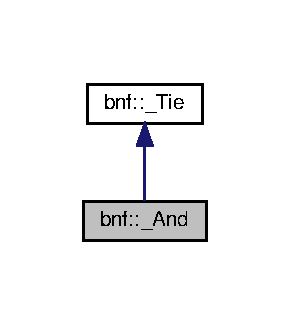
\includegraphics[width=139pt]{classbnf_1_1___and__inherit__graph}
\end{center}
\end{figure}


Collaboration diagram for bnf\+:\+:\+\_\+\+And\+:
\nopagebreak
\begin{figure}[H]
\begin{center}
\leavevmode
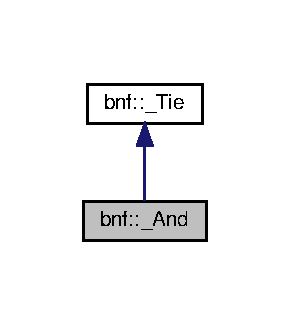
\includegraphics[width=139pt]{classbnf_1_1___and__coll__graph}
\end{center}
\end{figure}
\subsection*{Public Member Functions}
\begin{DoxyCompactItemize}
\item 
\mbox{\label{classbnf_1_1___and_af54576e9ade3afb5e1c1c0a36420596c}} 
\textbf{ \+\_\+\+And} \& {\bfseries operator+} (const \textbf{ \+\_\+\+Tie} \&rule2)
\item 
\mbox{\label{classbnf_1_1___and_ada6a76d66b9183ae9ba3ea834ea062eb}} 
\textbf{ \+\_\+\+And} \& {\bfseries operator+} (const char $\ast$s)
\item 
\mbox{\label{classbnf_1_1___and_afa5d2abd30d243c35566ee2597ebebf1}} 
\textbf{ \+\_\+\+And} \& {\bfseries operator+} (bool($\ast$f)(const char $\ast$, size\+\_\+t))
\end{DoxyCompactItemize}
\subsection*{Protected Member Functions}
\begin{DoxyCompactItemize}
\item 
\mbox{\label{classbnf_1_1___and_ae3d8900b2c6b0d8f0c12b5599db4e225}} 
{\bfseries \+\_\+\+And} (const \textbf{ \+\_\+\+Tie} \&b1, const \textbf{ \+\_\+\+Tie} \&b2)
\item 
\mbox{\label{classbnf_1_1___and_a87b30db4759ec37a1919439938d9c84b}} 
{\bfseries \+\_\+\+And} (const \textbf{ \+\_\+\+And} $\ast$rl)
\item 
\mbox{\label{classbnf_1_1___and_a75af45415ecbf1598ca1a73323d353fd}} 
virtual int {\bfseries \+\_\+parse} (\textbf{ \+\_\+\+Base} $\ast$parser) const  throw ()
\end{DoxyCompactItemize}
\subsection*{Friends}
\begin{DoxyCompactItemize}
\item 
\mbox{\label{classbnf_1_1___and_ab555bd08f573aad86ad95feb76007c15}} 
class {\bfseries \+\_\+\+Tie}
\item 
\mbox{\label{classbnf_1_1___and_a5e39c58451938ac9fc35e0ac18674f12}} 
class {\bfseries Lexem}
\item 
\mbox{\label{classbnf_1_1___and_ab3401f2dc96763fd3fde6f7cb61dbccb}} 
\textbf{ \+\_\+\+And} {\bfseries operator+} (const char $\ast$s, const \textbf{ \+\_\+\+Tie} \&link)
\item 
\mbox{\label{classbnf_1_1___and_aa6647834f11af3c454b2ada531a221e4}} 
\textbf{ \+\_\+\+And} {\bfseries operator+} (bool($\ast$f)(const char $\ast$, size\+\_\+t), const \textbf{ \+\_\+\+Tie} \&link)
\end{DoxyCompactItemize}
\subsection*{Additional Inherited Members}


The documentation for this class was generated from the following file\+:\begin{DoxyCompactItemize}
\item 
model/reco\+Plan/\+P\+A\+R\+C/include/bnflite.\+h\end{DoxyCompactItemize}

\section{bnf\+:\+:\+\_\+\+Base Class Reference}
\label{classbnf_1_1___base}\index{bnf\+::\+\_\+\+Base@{bnf\+::\+\_\+\+Base}}


Inheritance diagram for bnf\+:\+:\+\_\+\+Base\+:
\nopagebreak
\begin{figure}[H]
\begin{center}
\leavevmode
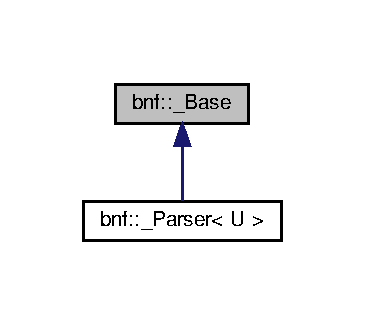
\includegraphics[width=175pt]{classbnf_1_1___base__inherit__graph}
\end{center}
\end{figure}
\subsection*{Public Member Functions}
\begin{DoxyCompactItemize}
\item 
\mbox{\label{classbnf_1_1___base_aefdb796fdec5b4172924717aa934dc4a}} 
int {\bfseries \+\_\+analyze} (\textbf{ \+\_\+\+Tie} \&root, const char $\ast$text, size\+\_\+t $\ast$)
\item 
\mbox{\label{classbnf_1_1___base_aabf499c8688286f6be285b89f101b720}} 
{\bfseries \+\_\+\+Base} (const char $\ast$($\ast$pre)(const char $\ast$))
\end{DoxyCompactItemize}
\subsection*{Static Public Member Functions}
\begin{DoxyCompactItemize}
\item 
\mbox{\label{classbnf_1_1___base_a3e28ced9cdb3f0443bcee04031fc49c9}} 
static const char $\ast$ {\bfseries base\+\_\+parser} (const char $\ast$ptr)
\item 
\mbox{\label{classbnf_1_1___base_a2f5856c7ff0791a7d9b9dbc0fc2c0fa7}} 
static int {\bfseries base\+\_\+error} (const char $\ast$ptr)
\end{DoxyCompactItemize}
\subsection*{Public Attributes}
\begin{DoxyCompactItemize}
\item 
\mbox{\label{classbnf_1_1___base_a305816876d6e007b3216289fa5cb763b}} 
std\+::vector$<$ const char $\ast$ $>$ {\bfseries cntxV}
\end{DoxyCompactItemize}
\subsection*{Protected Member Functions}
\begin{DoxyCompactItemize}
\item 
\mbox{\label{classbnf_1_1___base_a24b2c70e93327da9f342c11f7a8a61d1}} 
virtual void {\bfseries \+\_\+erase} (int low, int up=0)
\item 
\mbox{\label{classbnf_1_1___base_a00e146f614347f5cd256da4972b2b021}} 
virtual std\+::pair$<$ void $\ast$, int $>$ {\bfseries \+\_\+pre\+\_\+call} (void $\ast$callback)
\item 
\mbox{\label{classbnf_1_1___base_ab1a1132dd9a8294a9ec7ae9e9d908f2b}} 
virtual void {\bfseries \+\_\+post\+\_\+call} (std\+::pair$<$ void $\ast$, int $>$ up)
\item 
\mbox{\label{classbnf_1_1___base_ac63cafa36d2b032f030950622b59bde7}} 
virtual void {\bfseries \+\_\+do\+\_\+call} (std\+::pair$<$ void $\ast$, int $>$ up, void $\ast$callback, const char $\ast$begin, const char $\ast$end, const char $\ast$name)
\item 
\mbox{\label{classbnf_1_1___base_a088e0841175a63af7d6867728fb67857}} 
virtual void {\bfseries \+\_\+stub\+\_\+call} (const char $\ast$begin, const char $\ast$end, const char $\ast$name)
\end{DoxyCompactItemize}
\subsection*{Protected Attributes}
\begin{DoxyCompactItemize}
\item 
\mbox{\label{classbnf_1_1___base_a453778efab1591833f58f9e87ce1847c}} 
int {\bfseries level}
\item 
\mbox{\label{classbnf_1_1___base_a2c4c10392aceaaae362f05a10c76ee95}} 
const char $\ast$($\ast$ {\bfseries zero\+\_\+parse} )(const char $\ast$)
\item 
\mbox{\label{classbnf_1_1___base_afbb5aeec84c9cea8874db4d3f6911ce9}} 
int($\ast$ {\bfseries catch\+\_\+error} )(const char $\ast$ptr)
\end{DoxyCompactItemize}
\subsection*{Friends}
\begin{DoxyCompactItemize}
\item 
\mbox{\label{classbnf_1_1___base_a48f5c1ca47af8dc65eca7e0274de96e2}} 
class {\bfseries Token}
\item 
\mbox{\label{classbnf_1_1___base_a5e39c58451938ac9fc35e0ac18674f12}} 
class {\bfseries Lexem}
\item 
\mbox{\label{classbnf_1_1___base_a6c87f8640d92f86217b1b5ac79943269}} 
class {\bfseries Rule}
\item 
\mbox{\label{classbnf_1_1___base_abc37899b09eb024e8e57c00ec8fba682}} 
class {\bfseries \+\_\+\+And}
\item 
\mbox{\label{classbnf_1_1___base_abc2ecc13a8a23716fb474fcc5d47a88f}} 
class {\bfseries \+\_\+\+Or}
\end{DoxyCompactItemize}


The documentation for this class was generated from the following file\+:\begin{DoxyCompactItemize}
\item 
model/reco\+Plan/\+P\+A\+R\+C/include/bnflite.\+h\end{DoxyCompactItemize}

\section{bnf\+:\+:\+\_\+\+Ctrl$<$ flg, cc $>$ Class Template Reference}
\label{classbnf_1_1___ctrl}\index{bnf\+::\+\_\+\+Ctrl$<$ flg, cc $>$@{bnf\+::\+\_\+\+Ctrl$<$ flg, cc $>$}}


Inheritance diagram for bnf\+:\+:\+\_\+\+Ctrl$<$ flg, cc $>$\+:
\nopagebreak
\begin{figure}[H]
\begin{center}
\leavevmode
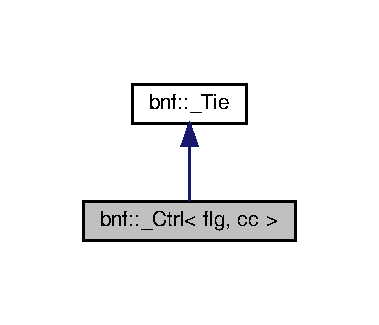
\includegraphics[width=182pt]{classbnf_1_1___ctrl__inherit__graph}
\end{center}
\end{figure}


Collaboration diagram for bnf\+:\+:\+\_\+\+Ctrl$<$ flg, cc $>$\+:
\nopagebreak
\begin{figure}[H]
\begin{center}
\leavevmode
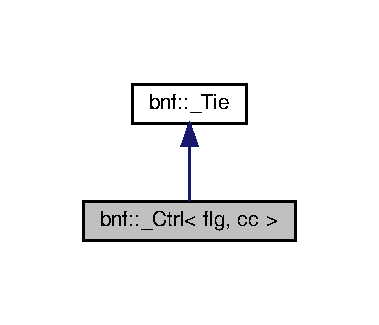
\includegraphics[width=182pt]{classbnf_1_1___ctrl__coll__graph}
\end{center}
\end{figure}
\subsection*{Protected Member Functions}
\begin{DoxyCompactItemize}
\item 
\mbox{\label{classbnf_1_1___ctrl_adbaef05a183046207b717abbc5e3e815}} 
virtual int {\bfseries \+\_\+parse} (\textbf{ \+\_\+\+Base} $\ast$parser) const  throw ()
\item 
\mbox{\label{classbnf_1_1___ctrl_a176955339cc1cac3ce06070a3d2f3d90}} 
{\bfseries \+\_\+\+Ctrl} (const \textbf{ \+\_\+\+Ctrl} $\ast$ctrl)
\item 
\mbox{\label{classbnf_1_1___ctrl_aa6195bf31c3d0c9496d7e2e83cc923c4}} 
{\bfseries \+\_\+\+Ctrl} (const \textbf{ \+\_\+\+Ctrl} \&control)
\end{DoxyCompactItemize}
\subsection*{Friends}
\begin{DoxyCompactItemize}
\item 
\mbox{\label{classbnf_1_1___ctrl_ab555bd08f573aad86ad95feb76007c15}} 
class {\bfseries \+\_\+\+Tie}
\end{DoxyCompactItemize}
\subsection*{Additional Inherited Members}


The documentation for this class was generated from the following file\+:\begin{DoxyCompactItemize}
\item 
model/reco\+Plan/\+P\+A\+R\+C/include/bnflite.\+h\end{DoxyCompactItemize}

\section{bnf\+:\+:\+\_\+\+Cycle Class Reference}
\label{classbnf_1_1___cycle}\index{bnf\+::\+\_\+\+Cycle@{bnf\+::\+\_\+\+Cycle}}


Inheritance diagram for bnf\+:\+:\+\_\+\+Cycle\+:
\nopagebreak
\begin{figure}[H]
\begin{center}
\leavevmode
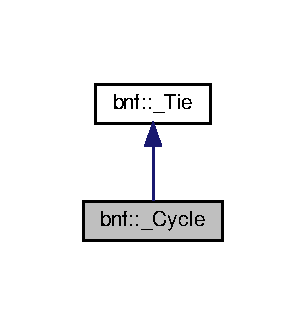
\includegraphics[width=147pt]{classbnf_1_1___cycle__inherit__graph}
\end{center}
\end{figure}


Collaboration diagram for bnf\+:\+:\+\_\+\+Cycle\+:
\nopagebreak
\begin{figure}[H]
\begin{center}
\leavevmode
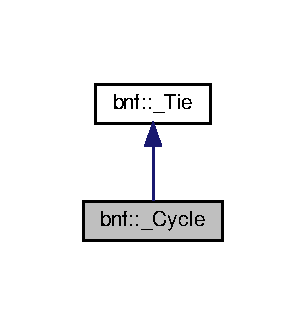
\includegraphics[width=147pt]{classbnf_1_1___cycle__coll__graph}
\end{center}
\end{figure}
\subsection*{Protected Member Functions}
\begin{DoxyCompactItemize}
\item 
\mbox{\label{classbnf_1_1___cycle_a4c0920f51b63a6e78f5c2b117bf2c81b}} 
{\bfseries \+\_\+\+Cycle} (const \textbf{ \+\_\+\+Cycle} $\ast$cl)
\item 
\mbox{\label{classbnf_1_1___cycle_acf425c301789e1e7f7dda3685a869b96}} 
{\bfseries \+\_\+\+Cycle} (const \textbf{ \+\_\+\+Cycle} \&cycle)
\item 
\mbox{\label{classbnf_1_1___cycle_adb2e2eaec3ddc1bce09855229cb5f2ca}} 
int {\bfseries \+\_\+parse} (\textbf{ \+\_\+\+Base} $\ast$parser) const  throw ()
\item 
\mbox{\label{classbnf_1_1___cycle_a2d6de9d3b4c142c1396d34ca2b0e8ae3}} 
{\bfseries \+\_\+\+Cycle} (int at\+\_\+least, const \textbf{ \+\_\+\+Tie} \&link, int total=max\+Iterate, int limit=max\+Iterate)
\end{DoxyCompactItemize}
\subsection*{Friends}
\begin{DoxyCompactItemize}
\item 
\mbox{\label{classbnf_1_1___cycle_ab555bd08f573aad86ad95feb76007c15}} 
class {\bfseries \+\_\+\+Tie}
\item 
\mbox{\label{classbnf_1_1___cycle_a42c2b33ba506a4cf0d9c52e320e471ae}} 
\textbf{ \+\_\+\+Cycle} {\bfseries operator$\ast$} (int x, const \textbf{ \+\_\+\+Tie} \&link)
\item 
\mbox{\label{classbnf_1_1___cycle_a8f5b6bfc935f03ffd6af67c00ed3c27e}} 
\textbf{ \+\_\+\+Cycle} {\bfseries Repeat} (int at\+\_\+least, const \textbf{ Rule} \&\textbf{ rule}, int total=max\+Lexem\+Length, int limit=max\+Lexem\+Length)
\item 
\mbox{\label{classbnf_1_1___cycle_a35464540445f3163727003daeebb8904}} 
\textbf{ \+\_\+\+Cycle} {\bfseries Iterate} (int at\+\_\+least, const \textbf{ Lexem} \&lexem, int total=max\+Lexem\+Length, int limit=max\+Lexem\+Length)
\item 
\mbox{\label{classbnf_1_1___cycle_a39253986f40d82c4455593c7afc3e426}} 
\textbf{ \+\_\+\+Cycle} {\bfseries Series} (int at\+\_\+least, const \textbf{ Token} \&token, int total=max\+Lexem\+Length, int limit=max\+Lexem\+Length)
\end{DoxyCompactItemize}
\subsection*{Additional Inherited Members}


The documentation for this class was generated from the following file\+:\begin{DoxyCompactItemize}
\item 
model/reco\+Plan/\+P\+A\+R\+C/include/bnflite.\+h\end{DoxyCompactItemize}

\section{bnf\+:\+:\+\_\+\+Or Class Reference}
\label{classbnf_1_1___or}\index{bnf\+::\+\_\+\+Or@{bnf\+::\+\_\+\+Or}}


Inheritance diagram for bnf\+:\+:\+\_\+\+Or\+:
\nopagebreak
\begin{figure}[H]
\begin{center}
\leavevmode
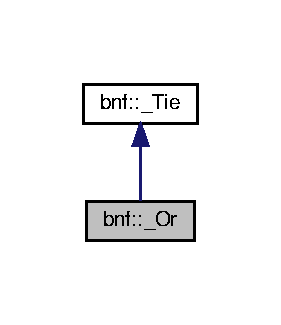
\includegraphics[width=135pt]{classbnf_1_1___or__inherit__graph}
\end{center}
\end{figure}


Collaboration diagram for bnf\+:\+:\+\_\+\+Or\+:
\nopagebreak
\begin{figure}[H]
\begin{center}
\leavevmode
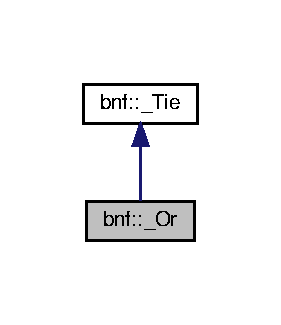
\includegraphics[width=135pt]{classbnf_1_1___or__coll__graph}
\end{center}
\end{figure}
\subsection*{Public Member Functions}
\begin{DoxyCompactItemize}
\item 
\mbox{\label{classbnf_1_1___or_ab50193a5c6b0bf1f8f61ba1fe2020187}} 
\textbf{ \+\_\+\+Or} \& {\bfseries operator$\vert$} (const \textbf{ \+\_\+\+Tie} \&rule2)
\item 
\mbox{\label{classbnf_1_1___or_a83447b5a8ad57757568a8f92795eae76}} 
\textbf{ \+\_\+\+Or} \& {\bfseries operator$\vert$} (const char $\ast$s)
\item 
\mbox{\label{classbnf_1_1___or_a23d0d9ca62283285457a6b7893399b0a}} 
\textbf{ \+\_\+\+Or} \& {\bfseries operator$\vert$} (bool($\ast$f)(const char $\ast$, size\+\_\+t))
\end{DoxyCompactItemize}
\subsection*{Protected Member Functions}
\begin{DoxyCompactItemize}
\item 
\mbox{\label{classbnf_1_1___or_a6dcf19923b57986807afbefc59f5565f}} 
{\bfseries \+\_\+\+Or} (const \textbf{ \+\_\+\+Tie} \&b1, const \textbf{ \+\_\+\+Tie} \&b2)
\item 
\mbox{\label{classbnf_1_1___or_ab00468b6e1f63a99bb9703ccf65f0179}} 
{\bfseries \+\_\+\+Or} (const \textbf{ \+\_\+\+Or} $\ast$rl)
\item 
\mbox{\label{classbnf_1_1___or_a47bf693c952f0cf06ed6ba0864efcd60}} 
virtual int {\bfseries \+\_\+parse} (\textbf{ \+\_\+\+Base} $\ast$parser) const  throw ()
\end{DoxyCompactItemize}
\subsection*{Friends}
\begin{DoxyCompactItemize}
\item 
\mbox{\label{classbnf_1_1___or_ab555bd08f573aad86ad95feb76007c15}} 
class {\bfseries \+\_\+\+Tie}
\item 
\mbox{\label{classbnf_1_1___or_a0065d8a2cc1f4d7c72a2a68baf5e9dcb}} 
\textbf{ \+\_\+\+Or} {\bfseries operator$\vert$} (const char $\ast$s, const \textbf{ \+\_\+\+Tie} \&link)
\item 
\mbox{\label{classbnf_1_1___or_a821e28de6bce22c0ad96966f406fe380}} 
\textbf{ \+\_\+\+Or} {\bfseries operator$\vert$} (bool($\ast$f)(const char $\ast$, size\+\_\+t), const \textbf{ \+\_\+\+Tie} \&link)
\end{DoxyCompactItemize}
\subsection*{Additional Inherited Members}


The documentation for this class was generated from the following file\+:\begin{DoxyCompactItemize}
\item 
model/reco\+Plan/\+P\+A\+R\+C/include/bnflite.\+h\end{DoxyCompactItemize}

\section{bnf\+:\+:\+\_\+\+Parser$<$ U $>$ Class Template Reference}
\label{classbnf_1_1___parser}\index{bnf\+::\+\_\+\+Parser$<$ U $>$@{bnf\+::\+\_\+\+Parser$<$ U $>$}}


Inheritance diagram for bnf\+:\+:\+\_\+\+Parser$<$ U $>$\+:
\nopagebreak
\begin{figure}[H]
\begin{center}
\leavevmode
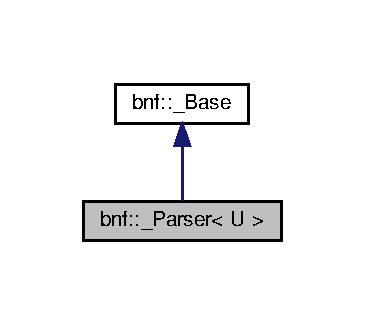
\includegraphics[width=175pt]{classbnf_1_1___parser__inherit__graph}
\end{center}
\end{figure}


Collaboration diagram for bnf\+:\+:\+\_\+\+Parser$<$ U $>$\+:
\nopagebreak
\begin{figure}[H]
\begin{center}
\leavevmode
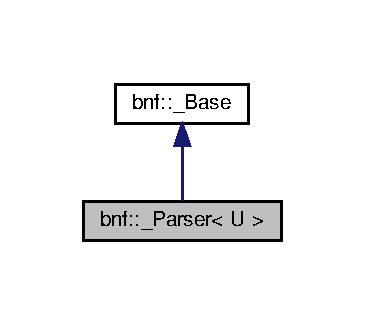
\includegraphics[width=175pt]{classbnf_1_1___parser__coll__graph}
\end{center}
\end{figure}
\subsection*{Public Member Functions}
\begin{DoxyCompactItemize}
\item 
\mbox{\label{classbnf_1_1___parser_ac57c83f59cec66d464ddbafd3b9b1347}} 
{\bfseries \+\_\+\+Parser} (const char $\ast$($\ast$f)(const char $\ast$), std\+::vector$<$ U $>$ $\ast$v)
\item 
\mbox{\label{classbnf_1_1___parser_a7b311aedf21877c4b11d13ac5c31a047}} 
int {\bfseries \+\_\+get\+\_\+result} (U \&u)
\end{DoxyCompactItemize}
\subsection*{Protected Member Functions}
\begin{DoxyCompactItemize}
\item 
\mbox{\label{classbnf_1_1___parser_a754b79ca6995630f49a825882c27236f}} 
void {\bfseries \+\_\+erase} (int low, int up=0)
\item 
\mbox{\label{classbnf_1_1___parser_a6d889544a678ade59c9c815fe0f4996a}} 
virtual std\+::pair$<$ void $\ast$, int $>$ {\bfseries \+\_\+pre\+\_\+call} (void $\ast$callback)
\item 
\mbox{\label{classbnf_1_1___parser_a9ec77b1775499d4027944409c5d76d53}} 
virtual void {\bfseries \+\_\+post\+\_\+call} (std\+::pair$<$ void $\ast$, int $>$ up)
\item 
\mbox{\label{classbnf_1_1___parser_a8a7b530150d6d1d47394ac3d722cdc45}} 
virtual void {\bfseries \+\_\+do\+\_\+call} (std\+::pair$<$ void $\ast$, int $>$ up, void $\ast$callback, const char $\ast$begin, const char $\ast$end, const char $\ast$name)
\item 
\mbox{\label{classbnf_1_1___parser_a37cb39a6c1a50c12520b3305e373e898}} 
virtual void {\bfseries \+\_\+stub\+\_\+call} (const char $\ast$begin, const char $\ast$end, const char $\ast$name)
\end{DoxyCompactItemize}
\subsection*{Protected Attributes}
\begin{DoxyCompactItemize}
\item 
\mbox{\label{classbnf_1_1___parser_a3f445fa7138af0c8636db4ff88d3e810}} 
std\+::vector$<$ U $>$ $\ast$ {\bfseries cntxU}
\item 
\mbox{\label{classbnf_1_1___parser_a02e8109a611bf1157929b5c90df08a06}} 
unsigned int {\bfseries off}
\end{DoxyCompactItemize}
\subsection*{Friends}
\begin{DoxyCompactItemize}
\item 
\mbox{\label{classbnf_1_1___parser_ad8e6fd2316a4d552ad378a676daf243b}} 
{\footnotesize template$<$class W $>$ }\\\textbf{ Rule} \& {\bfseries Bind} (\textbf{ Rule} \&\textbf{ rule}, W($\ast$callback)(std\+::vector$<$ W $>$ \&))
\end{DoxyCompactItemize}
\subsection*{Additional Inherited Members}


The documentation for this class was generated from the following file\+:\begin{DoxyCompactItemize}
\item 
model/reco\+Plan/\+P\+A\+R\+C/include/bnflite.\+h\end{DoxyCompactItemize}

\section{bnf\+:\+:\+\_\+\+Tie Class Reference}
\label{classbnf_1_1___tie}\index{bnf\+::\+\_\+\+Tie@{bnf\+::\+\_\+\+Tie}}


Inheritance diagram for bnf\+:\+:\+\_\+\+Tie\+:
\nopagebreak
\begin{figure}[H]
\begin{center}
\leavevmode
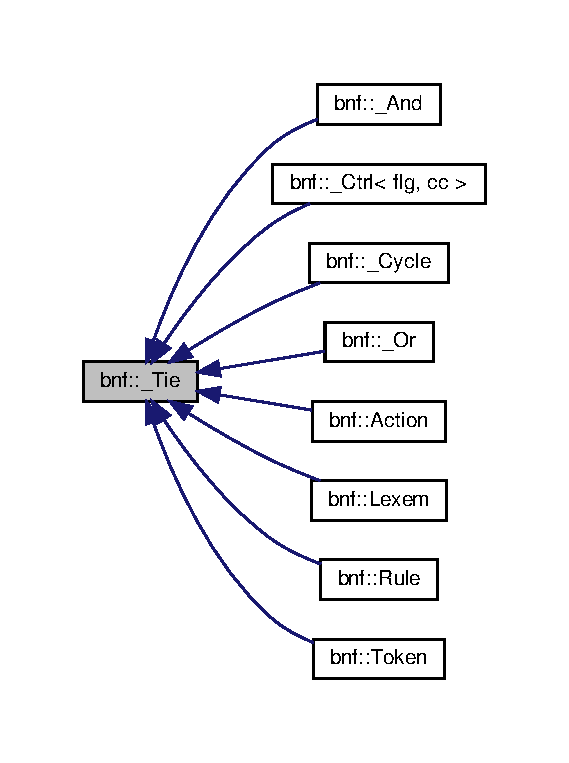
\includegraphics[width=273pt]{classbnf_1_1___tie__inherit__graph}
\end{center}
\end{figure}
\subsection*{Public Member Functions}
\begin{DoxyCompactItemize}
\item 
\mbox{\label{classbnf_1_1___tie_ac647ba15a4aee726c7995c611db02492}} 
void {\bfseries set\+Name} (const char $\ast$name)
\item 
\mbox{\label{classbnf_1_1___tie_a5ada30dfe6ddee89e0fc1f590be13266}} 
const char $\ast$ {\bfseries get\+Name} ()
\item 
\mbox{\label{classbnf_1_1___tie_ace83835bbee0790d181ed4de97086aea}} 
\textbf{ \+\_\+\+And} {\bfseries operator+} (const \textbf{ \+\_\+\+Tie} \&link)
\item 
\mbox{\label{classbnf_1_1___tie_ae6275d0d44f0edd915b5a8709a317017}} 
\textbf{ \+\_\+\+And} {\bfseries operator+} (const char $\ast$s)
\item 
\mbox{\label{classbnf_1_1___tie_a7fcf8ccdc485bfd1bf8d5f187ccadcee}} 
\textbf{ \+\_\+\+And} {\bfseries operator+} (bool($\ast$f)(const char $\ast$, size\+\_\+t))
\item 
\mbox{\label{classbnf_1_1___tie_a0fb85544a86647ff1db09eabe235d730}} 
\textbf{ \+\_\+\+Or} {\bfseries operator$\vert$} (const \textbf{ \+\_\+\+Tie} \&link)
\item 
\mbox{\label{classbnf_1_1___tie_ab5624a8f40f51c8eeb96ec1a47cccce6}} 
\textbf{ \+\_\+\+Or} {\bfseries operator$\vert$} (const char $\ast$s)
\item 
\mbox{\label{classbnf_1_1___tie_af1b6229c7c9c3975b82edbfb5c92ef24}} 
\textbf{ \+\_\+\+Or} {\bfseries operator$\vert$} (bool($\ast$f)(const char $\ast$, size\+\_\+t))
\item 
\mbox{\label{classbnf_1_1___tie_a787b666fa012e38d60e04b46c2ad01ef}} 
\textbf{ \+\_\+\+Cycle} {\bfseries operator()} (int at\+\_\+least, int total)
\item 
\mbox{\label{classbnf_1_1___tie_a2c5e2c656a996cfefff611ac533be9c1}} 
\textbf{ \+\_\+\+Cycle} {\bfseries operator$\ast$} ()
\item 
\mbox{\label{classbnf_1_1___tie_afdd94b85872f795af274e258e66396e7}} 
\textbf{ \+\_\+\+Cycle} {\bfseries operator!} ()
\end{DoxyCompactItemize}
\subsection*{Protected Member Functions}
\begin{DoxyCompactItemize}
\item 
\mbox{\label{classbnf_1_1___tie_ae1a6db1009a1212f8d9297446dea3af5}} 
void {\bfseries \+\_\+clone} (const \textbf{ \+\_\+\+Tie} $\ast$lnk)
\item 
\mbox{\label{classbnf_1_1___tie_a5acb87106d25769797a347fba072dcbd}} 
{\bfseries \+\_\+\+Tie} (std\+::string nm=\char`\"{}\char`\"{})
\item 
\mbox{\label{classbnf_1_1___tie_a4fea3452db346af8ff973c94068f3e4a}} 
{\bfseries \+\_\+\+Tie} (const \textbf{ \+\_\+\+Tie} $\ast$lnk)
\item 
\mbox{\label{classbnf_1_1___tie_a1d2910459130d3377281fe40053b8b72}} 
{\bfseries \+\_\+\+Tie} (const \textbf{ \+\_\+\+Tie} \&link)
\item 
\mbox{\label{classbnf_1_1___tie_a76631238fac475a2a9b6adfe8e31b529}} 
void {\bfseries \+\_\+clue} (const \textbf{ \+\_\+\+Tie} \&link)
\item 
\mbox{\label{classbnf_1_1___tie_a3ef41cf1dbd1d28f3f1ab22256ea3bd8}} 
virtual int {\bfseries \+\_\+parse} (\textbf{ \+\_\+\+Base} $\ast$parser) const =0  throw ()
\end{DoxyCompactItemize}
\subsection*{Static Protected Member Functions}
\begin{DoxyCompactItemize}
\item 
\mbox{\label{classbnf_1_1___tie_a2e6c961a8607120b153024a83bf7e046}} 
{\footnotesize template$<$class T $>$ }\\static void {\bfseries \+\_\+setname} (T $\ast$t, const char $\ast$name=0)
\item 
\mbox{\label{classbnf_1_1___tie_af1bc0dc1dfc73e91de8d3aef513b12e0}} 
static int {\bfseries call\+\_\+1st} (const \textbf{ \+\_\+\+Tie} $\ast$lnk, \textbf{ \+\_\+\+Base} $\ast$parser)
\item 
\mbox{\label{classbnf_1_1___tie_ade0d3607f99af81e30b336bf73087b8e}} 
{\footnotesize template$<$class T $>$ }\\static T $\ast$ {\bfseries \+\_\+safe\+\_\+delete} (T $\ast$t)
\end{DoxyCompactItemize}
\subsection*{Protected Attributes}
\begin{DoxyCompactItemize}
\item 
\mbox{\label{classbnf_1_1___tie_aaa82ae6741bf93468654c650fcb66675}} 
bool {\bfseries inner}
\item 
\mbox{\label{classbnf_1_1___tie_ad389488f34be5f98c813498a24274b7e}} 
std\+::vector$<$ const \textbf{ \+\_\+\+Tie} $\ast$ $>$ {\bfseries use}
\item 
\mbox{\label{classbnf_1_1___tie_a6de3678b6baf706a990d2da5f77e786e}} 
std\+::list$<$ const \textbf{ \+\_\+\+Tie} $\ast$ $>$ {\bfseries usage}
\item 
\mbox{\label{classbnf_1_1___tie_a3f421bf925f39f3c571fe97981dd82af}} 
std\+::string {\bfseries name}
\end{DoxyCompactItemize}
\subsection*{Friends}
\begin{DoxyCompactItemize}
\item 
\mbox{\label{classbnf_1_1___tie_acc4a46af6ba91f5c229096b7f622876a}} 
class {\bfseries \+\_\+\+Base}
\item 
\mbox{\label{classbnf_1_1___tie_a56aeb37d353745b814d576d4eee8bf58}} 
class {\bfseries Ext\+Parser}
\item 
\mbox{\label{classbnf_1_1___tie_abc37899b09eb024e8e57c00ec8fba682}} 
class {\bfseries \+\_\+\+And}
\item 
\mbox{\label{classbnf_1_1___tie_abc2ecc13a8a23716fb474fcc5d47a88f}} 
class {\bfseries \+\_\+\+Or}
\item 
\mbox{\label{classbnf_1_1___tie_a42b7257dd7b67cb080c28eed1201d5e2}} 
class {\bfseries \+\_\+\+Cycle}
\item 
\mbox{\label{classbnf_1_1___tie_a48f5c1ca47af8dc65eca7e0274de96e2}} 
class {\bfseries Token}
\item 
\mbox{\label{classbnf_1_1___tie_a5e39c58451938ac9fc35e0ac18674f12}} 
class {\bfseries Lexem}
\item 
\mbox{\label{classbnf_1_1___tie_a6c87f8640d92f86217b1b5ac79943269}} 
class {\bfseries Rule}
\item 
\mbox{\label{classbnf_1_1___tie_ae39b09ed012034d4a0ca5e90ec961764}} 
\textbf{ \+\_\+\+And} {\bfseries operator+} (const char $\ast$s, const \textbf{ \+\_\+\+Tie} \&lnk)
\item 
\mbox{\label{classbnf_1_1___tie_affdc9f825c9dea37493c32c4e5547cb3}} 
\textbf{ \+\_\+\+And} {\bfseries operator+} (bool($\ast$f)(const char $\ast$, size\+\_\+t), const \textbf{ \+\_\+\+Tie} \&lnk)
\item 
\mbox{\label{classbnf_1_1___tie_a13f77fb3c0e59327b41449c74cfca230}} 
\textbf{ \+\_\+\+Or} {\bfseries operator$\vert$} (const char $\ast$s, const \textbf{ \+\_\+\+Tie} \&lnk)
\item 
\mbox{\label{classbnf_1_1___tie_a49635d0b72696d3519c0e4993b6636d4}} 
\textbf{ \+\_\+\+Or} {\bfseries operator$\vert$} (bool($\ast$f)(const char $\ast$, size\+\_\+t), const \textbf{ \+\_\+\+Tie} \&lnk)
\end{DoxyCompactItemize}


The documentation for this class was generated from the following file\+:\begin{DoxyCompactItemize}
\item 
model/reco\+Plan/\+P\+A\+R\+C/include/bnflite.\+h\end{DoxyCompactItemize}

\section{bnf\+:\+:Action Class Reference}
\label{classbnf_1_1_action}\index{bnf\+::\+Action@{bnf\+::\+Action}}


Inheritance diagram for bnf\+:\+:Action\+:
\nopagebreak
\begin{figure}[H]
\begin{center}
\leavevmode
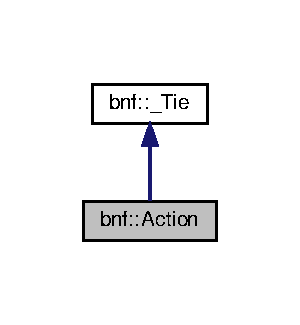
\includegraphics[width=144pt]{classbnf_1_1_action__inherit__graph}
\end{center}
\end{figure}


Collaboration diagram for bnf\+:\+:Action\+:
\nopagebreak
\begin{figure}[H]
\begin{center}
\leavevmode
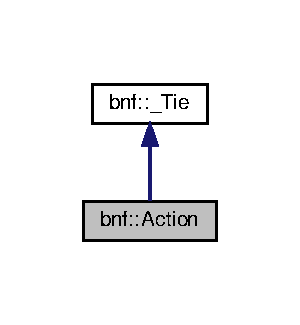
\includegraphics[width=144pt]{classbnf_1_1_action__coll__graph}
\end{center}
\end{figure}
\subsection*{Public Member Functions}
\begin{DoxyCompactItemize}
\item 
\mbox{\label{classbnf_1_1_action_a6c60ae74d4c9137caee753dbd4db02e6}} 
{\bfseries Action} (bool($\ast$action)(const char $\ast$lexem, size\+\_\+t len), const char $\ast$name=\char`\"{}\char`\"{})
\end{DoxyCompactItemize}
\subsection*{Protected Member Functions}
\begin{DoxyCompactItemize}
\item 
\mbox{\label{classbnf_1_1_action_a2e13af9e01185e0443815825f463349f}} 
{\bfseries Action} (const \textbf{ Action} $\ast$a)
\item 
\mbox{\label{classbnf_1_1_action_a59f61814edc11a5b513fb4fc10158543}} 
int {\bfseries \+\_\+parse} (\textbf{ \+\_\+\+Base} $\ast$parser) const  throw ()
\end{DoxyCompactItemize}
\subsection*{Friends}
\begin{DoxyCompactItemize}
\item 
\mbox{\label{classbnf_1_1_action_ab555bd08f573aad86ad95feb76007c15}} 
class {\bfseries \+\_\+\+Tie}
\end{DoxyCompactItemize}
\subsection*{Additional Inherited Members}


The documentation for this class was generated from the following file\+:\begin{DoxyCompactItemize}
\item 
model/reco\+Plan/\+P\+A\+R\+C/include/bnflite.\+h\end{DoxyCompactItemize}

\section{Activity\+Region Class Reference}
\label{class_activity_region}\index{Activity\+Region@{Activity\+Region}}
\subsection*{Public Member Functions}
\begin{DoxyCompactItemize}
\item 
\textbf{ Activity\+Region} (map$<$ string, string $>$ setting)
\begin{DoxyCompactList}\small\item\em Constructor of class \doxyref{Activity\+Region}{p.}{class_activity_region}. \end{DoxyCompactList}\item 
void \textbf{ Update} (cv\+::\+Mat vision, cv\+::\+Mat depth\+Vision)
\begin{DoxyCompactList}\small\item\em send to Y\+O\+LO image then update vector of Hands and Objects \end{DoxyCompactList}\item 
\textbf{ Detected\+Objects} \textbf{ detect\+Hand} (cv\+::\+Mat color, cv\+::\+Mat depth)
\begin{DoxyCompactList}\small\item\em from matrix of color and depth, found hands \end{DoxyCompactList}\item 
\textbf{ Detected\+Objects} \textbf{ detect\+Objets} (cv\+::\+Mat color, cv\+::\+Mat depth)
\begin{DoxyCompactList}\small\item\em from matrix of color and depth, found objects \end{DoxyCompactList}\item 
\mbox{\label{class_activity_region_aaedd12ffbb381ef845cd5aa72ed6826e}} 
void \textbf{ Update\+R\+OI} (cv\+::\+Mat vision, cv\+::\+Mat depth\+Vision)
\begin{DoxyCompactList}\small\item\em Y\+O\+LO I guess. \end{DoxyCompactList}\item 
\mbox{\label{class_activity_region_af55c48016552bc9438e7170a72ad8687}} 
void {\bfseries update\+Manual\+R\+OI} (cv\+::\+Mat vision, cv\+::\+Mat depth\+Vision, cv\+::\+Rect chosen\+R\+OI)
\item 
\mbox{\label{class_activity_region_a10c0391215447dfb4ae98fba2c89a1a1}} 
cv\+::\+Mat {\bfseries get\+Image\+With\+R\+OI} () const
\item 
\mbox{\label{class_activity_region_a2a5370220d07bc85f1ea716f8f3c57bb}} 
void \textbf{ reset} ()
\begin{DoxyCompactList}\small\item\em Reset vector of hands, objects, and regions. \end{DoxyCompactList}\item 
\mbox{\label{class_activity_region_a6bd9e8a428ebb079fd1d747ba5498b2a}} 
\textbf{ Detected\+Objects} \textbf{ get\+Hands} ()
\begin{DoxyCompactList}\small\item\em Getter. \end{DoxyCompactList}\item 
\mbox{\label{class_activity_region_a4f5e2d307274c28c5ce699f7621ab5f6}} 
\textbf{ Detected\+Objects} {\bfseries get\+Items} ()
\end{DoxyCompactItemize}
\subsection*{Static Public Member Functions}
\begin{DoxyCompactItemize}
\item 
static \textbf{ Activity\+Region} $\ast$ \textbf{ instance} (map$<$ string, string $>$ setting)
\begin{DoxyCompactList}\small\item\em check if \doxyref{Activity\+Region}{p.}{class_activity_region} object exist, else create it, then return it \end{DoxyCompactList}\end{DoxyCompactItemize}
\subsection*{Public Attributes}
\begin{DoxyCompactItemize}
\item 
\mbox{\label{class_activity_region_adde853c35d4b63094570ca276867a94e}} 
std\+::mutex \textbf{ mtx}
\begin{DoxyCompactList}\small\item\em public variables \end{DoxyCompactList}\end{DoxyCompactItemize}
\subsection*{Friends}
\begin{DoxyCompactItemize}
\item 
\mbox{\label{class_activity_region_ada1bc74916bf73465a08634c5178ec30}} 
class {\bfseries Primary\+Window}
\end{DoxyCompactItemize}


\subsection{Constructor \& Destructor Documentation}
\mbox{\label{class_activity_region_a2f202193c7944ed13d0188af8a0cfca7}} 
\index{Activity\+Region@{Activity\+Region}!Activity\+Region@{Activity\+Region}}
\index{Activity\+Region@{Activity\+Region}!Activity\+Region@{Activity\+Region}}
\subsubsection{Activity\+Region()}
{\footnotesize\ttfamily Activity\+Region\+::\+Activity\+Region (\begin{DoxyParamCaption}\item[{map$<$ string, string $>$}]{setting }\end{DoxyParamCaption})}



Constructor of class \doxyref{Activity\+Region}{p.}{class_activity_region}. 


\begin{DoxyParams}{Parameters}
{\em setting} & \+: map$<$string,string$>$ which contain every path and information to use (fisrt String = name\+\_\+of\+\_\+information, second String = information) \\
\hline
\end{DoxyParams}


\subsection{Member Function Documentation}
\mbox{\label{class_activity_region_a2975005c4e59a86dd21f9ac8da394d29}} 
\index{Activity\+Region@{Activity\+Region}!detect\+Hand@{detect\+Hand}}
\index{detect\+Hand@{detect\+Hand}!Activity\+Region@{Activity\+Region}}
\subsubsection{detect\+Hand()}
{\footnotesize\ttfamily \textbf{ Detected\+Objects} Activity\+Region\+::detect\+Hand (\begin{DoxyParamCaption}\item[{cv\+::\+Mat}]{color,  }\item[{cv\+::\+Mat}]{depth }\end{DoxyParamCaption})}



from matrix of color and depth, found hands 

Use Y\+O\+LO 
\begin{DoxyParams}{Parameters}
{\em vision} & \+: matrice which represent color of the picture \\
\hline
{\em depth\+Vision} & \+: matrice which represent the depth in the picture \\
\hline
\end{DoxyParams}
\begin{DoxyReturn}{Returns}
\doxyref{Detected\+Objects}{p.}{class_detected_objects} every hands that cnn have found 
\end{DoxyReturn}
\mbox{\label{class_activity_region_a6cc3ac4cd2d6e39367121776fc2e0437}} 
\index{Activity\+Region@{Activity\+Region}!detect\+Objets@{detect\+Objets}}
\index{detect\+Objets@{detect\+Objets}!Activity\+Region@{Activity\+Region}}
\subsubsection{detect\+Objets()}
{\footnotesize\ttfamily \textbf{ Detected\+Objects} Activity\+Region\+::detect\+Objets (\begin{DoxyParamCaption}\item[{cv\+::\+Mat}]{color,  }\item[{cv\+::\+Mat}]{depth }\end{DoxyParamCaption})}



from matrix of color and depth, found objects 

Use Y\+O\+LO 
\begin{DoxyParams}{Parameters}
{\em vision} & \+: matrix which represent color of the picture \\
\hline
{\em depth\+Vision} & \+: matrix which represent the depth in the picture \\
\hline
\end{DoxyParams}
\begin{DoxyReturn}{Returns}
\doxyref{Detected\+Objects}{p.}{class_detected_objects} \+: every pbjects that cnn have found 
\end{DoxyReturn}
\mbox{\label{class_activity_region_a92a746c743f639a177c4f3a48b39420c}} 
\index{Activity\+Region@{Activity\+Region}!instance@{instance}}
\index{instance@{instance}!Activity\+Region@{Activity\+Region}}
\subsubsection{instance()}
{\footnotesize\ttfamily \textbf{ Activity\+Region} $\ast$ Activity\+Region\+::instance (\begin{DoxyParamCaption}\item[{map$<$ string, string $>$}]{setting }\end{DoxyParamCaption})\hspace{0.3cm}{\ttfamily [inline]}, {\ttfamily [static]}}



check if \doxyref{Activity\+Region}{p.}{class_activity_region} object exist, else create it, then return it 

if it\textquotesingle{}s the first step of the loop (Mise\+A\+Jour\+Image) or pointer of \doxyref{Activity\+Region}{p.}{class_activity_region} as been delete 
\begin{DoxyParams}{Parameters}
{\em setting} & \+: map$<$string,string$>$ which contain every path and information to use (fisrt String = name\+\_\+of\+\_\+information, second String = information) \\
\hline
\end{DoxyParams}
\begin{DoxyReturn}{Returns}
Activity\+Region\+::ar\+\_\+instance \+: object of \doxyref{Activity\+Region}{p.}{class_activity_region} 
\end{DoxyReturn}
\mbox{\label{class_activity_region_aad8005109904e86239656d558720b198}} 
\index{Activity\+Region@{Activity\+Region}!Update@{Update}}
\index{Update@{Update}!Activity\+Region@{Activity\+Region}}
\subsubsection{Update()}
{\footnotesize\ttfamily void Activity\+Region\+::\+Update (\begin{DoxyParamCaption}\item[{cv\+::\+Mat}]{vision,  }\item[{cv\+::\+Mat}]{depth\+Vision }\end{DoxyParamCaption})}



send to Y\+O\+LO image then update vector of Hands and Objects 


\begin{DoxyParams}{Parameters}
{\em vision} & \+: matrice which represent color of the picture \\
\hline
{\em depth\+Vision} & \+: matrice which represent the depth in the picture \\
\hline
\end{DoxyParams}


The documentation for this class was generated from the following files\+:\begin{DoxyCompactItemize}
\item 
model/reco\+Activite/reco\+Image/\textbf{ Activity\+Region.\+h}\item 
model/reco\+Activite/reco\+Image/Activity\+Region.\+cpp\end{DoxyCompactItemize}

\section{Affordance Class Reference}
\label{class_affordance}\index{Affordance@{Affordance}}
\subsection*{Public Member Functions}
\begin{DoxyCompactItemize}
\item 
\textbf{ Affordance} (std\+::string obj=\char`\"{}teacup\char`\"{}, double prob=76.\+7653)
\begin{DoxyCompactList}\small\item\em Constructor of \doxyref{Affordance}{p.}{class_affordance}. \end{DoxyCompactList}\item 
\textbf{ Affordance} (std\+::string obj, double pos, cv\+::\+Rect reg, double prob, double \+\_\+dist=0)
\begin{DoxyCompactList}\small\item\em Constructor of \doxyref{Affordance}{p.}{class_affordance}. \end{DoxyCompactList}\item 
\mbox{\label{class_affordance_a1df2b93a131f51a9ec09543c3e90a973}} 
std\+::string {\bfseries get\+Name} () const
\item 
\mbox{\label{class_affordance_ae0af285b48f141b9a562be0dce29c118}} 
double {\bfseries get\+Object\+Position} () const
\item 
\mbox{\label{class_affordance_a946913b09e3996204b38e6ec95760927}} 
const cv\+::\+Rect \& {\bfseries get\+Region} () const
\item 
\mbox{\label{class_affordance_a0d994c5c809aba784d58eb855db218e0}} 
double {\bfseries get\+Object\+Probability} () const
\item 
\mbox{\label{class_affordance_acb92606601365f5fc88cd35d95fe9ef5}} 
void {\bfseries set\+Dist} (double dist)
\item 
\mbox{\label{class_affordance_a9ac80d93d6e91a45ac4167f0e59d6672}} 
void {\bfseries reset} ()
\item 
bool \textbf{ operator==} (const \textbf{ Affordance} \&autre)
\begin{DoxyCompactList}\small\item\em Overload of the \textquotesingle{}==\textquotesingle{} operator for two \doxyref{Affordance}{p.}{class_affordance} objects. \end{DoxyCompactList}\item 
bool \textbf{ operator$<$} (const \textbf{ Affordance} \&autre)
\begin{DoxyCompactList}\small\item\em Overload of the \textquotesingle{}$<$\textquotesingle{} operator for two \doxyref{Affordance}{p.}{class_affordance} objects. \end{DoxyCompactList}\item 
std\+::string \textbf{ to\+\_\+str} () const
\end{DoxyCompactItemize}
\subsection*{Friends}
\begin{DoxyCompactItemize}
\item 
\mbox{\label{class_affordance_a1d761ec04ad58029e54101c201c15d89}} 
std\+::ostream \& {\bfseries operator$<$$<$} (std\+::ostream \&o, const \textbf{ Affordance} a)
\end{DoxyCompactItemize}


\subsection{Constructor \& Destructor Documentation}
\mbox{\label{class_affordance_af5eb0d211b08c5e74bda3d278f4c0c36}} 
\index{Affordance@{Affordance}!Affordance@{Affordance}}
\index{Affordance@{Affordance}!Affordance@{Affordance}}
\subsubsection{Affordance()\hspace{0.1cm}{\footnotesize\ttfamily [1/2]}}
{\footnotesize\ttfamily Affordance\+::\+Affordance (\begin{DoxyParamCaption}\item[{std\+::string}]{obj = {\ttfamily \char`\"{}teacup\char`\"{}},  }\item[{double}]{prob = {\ttfamily 76.7653} }\end{DoxyParamCaption})}



Constructor of \doxyref{Affordance}{p.}{class_affordance}. 


\begin{DoxyParams}{Parameters}
{\em obj} & Name of the new Object \\
\hline
{\em prob} & Confidence rate on the object \\
\hline
\end{DoxyParams}
\mbox{\label{class_affordance_a7a5b691f83565f6905dabd64b80f8312}} 
\index{Affordance@{Affordance}!Affordance@{Affordance}}
\index{Affordance@{Affordance}!Affordance@{Affordance}}
\subsubsection{Affordance()\hspace{0.1cm}{\footnotesize\ttfamily [2/2]}}
{\footnotesize\ttfamily Affordance\+::\+Affordance (\begin{DoxyParamCaption}\item[{std\+::string}]{obj,  }\item[{double}]{pos,  }\item[{cv\+::\+Rect}]{reg,  }\item[{double}]{prob,  }\item[{double}]{\+\_\+dist = {\ttfamily 0} }\end{DoxyParamCaption})}



Constructor of \doxyref{Affordance}{p.}{class_affordance}. 


\begin{DoxyParams}{Parameters}
{\em obj} & String \+: Name of the new Object \\
\hline
{\em pos} & double \+: position of the Object at Creation \\
\hline
{\em reg} & cv\+::\+Rect \+: Open\+Cv class for 2D rectangles \\
\hline
{\em prob} & double \+: Confidence rate on the object \\
\hline
{\em dist} & double \+: Distance between the Hand and the Object \\
\hline
\end{DoxyParams}


\subsection{Member Function Documentation}
\mbox{\label{class_affordance_af080e51eb9ea5965c2cb0bee6caa4ff0}} 
\index{Affordance@{Affordance}!operator$<$@{operator$<$}}
\index{operator$<$@{operator$<$}!Affordance@{Affordance}}
\subsubsection{operator$<$()}
{\footnotesize\ttfamily bool Affordance\+::operator$<$ (\begin{DoxyParamCaption}\item[{const \textbf{ Affordance} \&}]{autre }\end{DoxyParamCaption})}



Overload of the \textquotesingle{}$<$\textquotesingle{} operator for two \doxyref{Affordance}{p.}{class_affordance} objects. 

\begin{DoxyReturn}{Returns}
True if this $<$ \textquotesingle{}autre\textquotesingle{} 
\end{DoxyReturn}
\mbox{\label{class_affordance_a4f7ff7d10b07287cb73c519689c60678}} 
\index{Affordance@{Affordance}!operator==@{operator==}}
\index{operator==@{operator==}!Affordance@{Affordance}}
\subsubsection{operator==()}
{\footnotesize\ttfamily bool Affordance\+::operator== (\begin{DoxyParamCaption}\item[{const \textbf{ Affordance} \&}]{autre }\end{DoxyParamCaption})}



Overload of the \textquotesingle{}==\textquotesingle{} operator for two \doxyref{Affordance}{p.}{class_affordance} objects. 

\begin{DoxyReturn}{Returns}
True if this == \textquotesingle{}autre\textquotesingle{} 
\end{DoxyReturn}
\mbox{\label{class_affordance_a0e999f7c0a400f4f1936c392843b5051}} 
\index{Affordance@{Affordance}!to\+\_\+str@{to\+\_\+str}}
\index{to\+\_\+str@{to\+\_\+str}!Affordance@{Affordance}}
\subsubsection{to\+\_\+str()}
{\footnotesize\ttfamily Affordance\+::to\+\_\+str (\begin{DoxyParamCaption}{ }\end{DoxyParamCaption}) const\hspace{0.3cm}{\ttfamily [inline]}}

\begin{DoxyReturn}{Returns}

\end{DoxyReturn}


The documentation for this class was generated from the following files\+:\begin{DoxyCompactItemize}
\item 
model/reco\+Activite/reco\+Affordance/\textbf{ Affordance.\+h}\item 
model/reco\+Activite/reco\+Affordance/Affordance.\+cpp\end{DoxyCompactItemize}

\section{Affordance\+Time Class Reference}
\label{class_affordance_time}\index{Affordance\+Time@{Affordance\+Time}}
\subsection*{Public Member Functions}
\begin{DoxyCompactItemize}
\item 
\mbox{\label{class_affordance_time_abe21e5e6200ceca2a4fd61498b1c5640}} 
\textbf{ Affordance\+Time} ()
\begin{DoxyCompactList}\small\item\em Constructor of \doxyref{Affordance\+Time}{p.}{class_affordance_time}. \end{DoxyCompactList}\item 
\textbf{ Affordance\+Time} (\textbf{ Affordance} aff, int frame\+Count)
\begin{DoxyCompactList}\small\item\em Constructor of \doxyref{Affordance\+Time}{p.}{class_affordance_time}. \end{DoxyCompactList}\item 
void \textbf{ mark\+Current\+Interactions} (double dist, int frame\+Count)
\begin{DoxyCompactList}\small\item\em Updates the \doxyref{Affordance}{p.}{class_affordance} object during an interaction. \end{DoxyCompactList}\item 
void \textbf{ mark\+Current\+Interactions} (double dist, cv\+::\+Rect pos, double prob, int frame\+Count)
\begin{DoxyCompactList}\small\item\em Updates the \doxyref{Affordance}{p.}{class_affordance} object during an interaction. \end{DoxyCompactList}\item 
double \textbf{ get\+Interaction\+Time} ()
\begin{DoxyCompactList}\small\item\em get\+Interaction\+Time \end{DoxyCompactList}\item 
double \textbf{ get\+Start\+Time} ()
\begin{DoxyCompactList}\small\item\em get\+Start\+Time \end{DoxyCompactList}\item 
\textbf{ Affordance} \& \textbf{ get\+Affordance} ()
\begin{DoxyCompactList}\small\item\em get\+Affordance \end{DoxyCompactList}\item 
std\+::string \textbf{ get\+Name} () const
\begin{DoxyCompactList}\small\item\em get\+Name \end{DoxyCompactList}\item 
int \textbf{ get\+Number\+Of\+Occurences} ()
\begin{DoxyCompactList}\small\item\em get\+Number\+Of\+Occurences \end{DoxyCompactList}\item 
\mbox{\label{class_affordance_time_ae822b9a1dd506d239476a71f1a4140c2}} 
void \textbf{ clean} ()
\begin{DoxyCompactList}\small\item\em Cleans the time attribute. \end{DoxyCompactList}\item 
\mbox{\label{class_affordance_time_a53f4750b6f9376cb38c4c88597a0e930}} 
void {\bfseries reset} ()
\item 
bool \textbf{ check\+Aff\+Name} (const std\+::string class\+Name) const
\begin{DoxyCompactList}\small\item\em check\+Aff\+Name \end{DoxyCompactList}\item 
bool \textbf{ operator==} (const \textbf{ Affordance\+Time} \&autre)
\begin{DoxyCompactList}\small\item\em Overload of the \textquotesingle{}==\textquotesingle{} operator for two \doxyref{Affordance\+Time}{p.}{class_affordance_time} objects. \end{DoxyCompactList}\item 
bool \textbf{ operator$<$} (const \textbf{ Affordance\+Time} \&autre)
\begin{DoxyCompactList}\small\item\em Overload of the \textquotesingle{}$<$\textquotesingle{} operator for two \doxyref{Affordance\+Time}{p.}{class_affordance_time} objects. \end{DoxyCompactList}\end{DoxyCompactItemize}
\subsection*{Friends}
\begin{DoxyCompactItemize}
\item 
\mbox{\label{class_affordance_time_ac4311c6b3409799833f5855b9c10b18f}} 
std\+::ostream \& {\bfseries operator$<$$<$} (std\+::ostream \&o, const \textbf{ Affordance\+Time} a)
\end{DoxyCompactItemize}


\subsection{Constructor \& Destructor Documentation}
\mbox{\label{class_affordance_time_a550d81ec8dc01717f6f3906d40022398}} 
\index{Affordance\+Time@{Affordance\+Time}!Affordance\+Time@{Affordance\+Time}}
\index{Affordance\+Time@{Affordance\+Time}!Affordance\+Time@{Affordance\+Time}}
\subsubsection{Affordance\+Time()}
{\footnotesize\ttfamily Affordance\+Time\+::\+Affordance\+Time (\begin{DoxyParamCaption}\item[{\textbf{ Affordance}}]{aff,  }\item[{int}]{frame\+Count }\end{DoxyParamCaption})}



Constructor of \doxyref{Affordance\+Time}{p.}{class_affordance_time}. 


\begin{DoxyParams}{Parameters}
{\em aff} & \doxyref{Affordance}{p.}{class_affordance} \+: Object of type \doxyref{Affordance}{p.}{class_affordance} \\
\hline
{\em frame\+Count} & int \+: Frame time at the creation \\
\hline
\end{DoxyParams}


\subsection{Member Function Documentation}
\mbox{\label{class_affordance_time_a115480f9cced506f442f100e1f3ca77d}} 
\index{Affordance\+Time@{Affordance\+Time}!check\+Aff\+Name@{check\+Aff\+Name}}
\index{check\+Aff\+Name@{check\+Aff\+Name}!Affordance\+Time@{Affordance\+Time}}
\subsubsection{check\+Aff\+Name()}
{\footnotesize\ttfamily bool Affordance\+Time\+::check\+Aff\+Name (\begin{DoxyParamCaption}\item[{const std\+::string}]{class\+Name }\end{DoxyParamCaption}) const\hspace{0.3cm}{\ttfamily [inline]}}



check\+Aff\+Name 


\begin{DoxyParams}{Parameters}
{\em class\+Name} & \\
\hline
\end{DoxyParams}
\begin{DoxyReturn}{Returns}

\end{DoxyReturn}
\mbox{\label{class_affordance_time_a4fcf18832933872e1a8a272fc089a97a}} 
\index{Affordance\+Time@{Affordance\+Time}!get\+Affordance@{get\+Affordance}}
\index{get\+Affordance@{get\+Affordance}!Affordance\+Time@{Affordance\+Time}}
\subsubsection{get\+Affordance()}
{\footnotesize\ttfamily \textbf{ Affordance}\& Affordance\+Time\+::get\+Affordance (\begin{DoxyParamCaption}{ }\end{DoxyParamCaption})\hspace{0.3cm}{\ttfamily [inline]}}



get\+Affordance 

\begin{DoxyReturn}{Returns}

\end{DoxyReturn}
\mbox{\label{class_affordance_time_a058273ed5117818c10adc82c1c489412}} 
\index{Affordance\+Time@{Affordance\+Time}!get\+Interaction\+Time@{get\+Interaction\+Time}}
\index{get\+Interaction\+Time@{get\+Interaction\+Time}!Affordance\+Time@{Affordance\+Time}}
\subsubsection{get\+Interaction\+Time()}
{\footnotesize\ttfamily double Affordance\+Time\+::get\+Interaction\+Time (\begin{DoxyParamCaption}{ }\end{DoxyParamCaption})\hspace{0.3cm}{\ttfamily [inline]}}



get\+Interaction\+Time 

\begin{DoxyReturn}{Returns}

\end{DoxyReturn}
\mbox{\label{class_affordance_time_af439cdc87988e29bbae0a036c37dc626}} 
\index{Affordance\+Time@{Affordance\+Time}!get\+Name@{get\+Name}}
\index{get\+Name@{get\+Name}!Affordance\+Time@{Affordance\+Time}}
\subsubsection{get\+Name()}
{\footnotesize\ttfamily std\+::string Affordance\+Time\+::get\+Name (\begin{DoxyParamCaption}{ }\end{DoxyParamCaption}) const\hspace{0.3cm}{\ttfamily [inline]}}



get\+Name 

\begin{DoxyReturn}{Returns}

\end{DoxyReturn}
\mbox{\label{class_affordance_time_a3290159565dbab9f17e94a59c3e9ffcf}} 
\index{Affordance\+Time@{Affordance\+Time}!get\+Number\+Of\+Occurences@{get\+Number\+Of\+Occurences}}
\index{get\+Number\+Of\+Occurences@{get\+Number\+Of\+Occurences}!Affordance\+Time@{Affordance\+Time}}
\subsubsection{get\+Number\+Of\+Occurences()}
{\footnotesize\ttfamily int Affordance\+Time\+::get\+Number\+Of\+Occurences (\begin{DoxyParamCaption}{ }\end{DoxyParamCaption})\hspace{0.3cm}{\ttfamily [inline]}}



get\+Number\+Of\+Occurences 

\begin{DoxyReturn}{Returns}

\end{DoxyReturn}
\mbox{\label{class_affordance_time_aef9d493b599b2d559a654e4a83596d3a}} 
\index{Affordance\+Time@{Affordance\+Time}!get\+Start\+Time@{get\+Start\+Time}}
\index{get\+Start\+Time@{get\+Start\+Time}!Affordance\+Time@{Affordance\+Time}}
\subsubsection{get\+Start\+Time()}
{\footnotesize\ttfamily double Affordance\+Time\+::get\+Start\+Time (\begin{DoxyParamCaption}{ }\end{DoxyParamCaption})\hspace{0.3cm}{\ttfamily [inline]}}



get\+Start\+Time 

\begin{DoxyReturn}{Returns}

\end{DoxyReturn}
\mbox{\label{class_affordance_time_ad8af5d283df25c5d3cfff186cde9abcf}} 
\index{Affordance\+Time@{Affordance\+Time}!mark\+Current\+Interactions@{mark\+Current\+Interactions}}
\index{mark\+Current\+Interactions@{mark\+Current\+Interactions}!Affordance\+Time@{Affordance\+Time}}
\subsubsection{mark\+Current\+Interactions()\hspace{0.1cm}{\footnotesize\ttfamily [1/2]}}
{\footnotesize\ttfamily Affordance\+Time\+::mark\+Current\+Interactions (\begin{DoxyParamCaption}\item[{double}]{dist,  }\item[{int}]{frame\+Count }\end{DoxyParamCaption})}



Updates the \doxyref{Affordance}{p.}{class_affordance} object during an interaction. 

Updates the \doxyref{Affordance}{p.}{class_affordance} object, called during an interaction Updates the current time and adds the frame time of the interaction 
\begin{DoxyParams}{Parameters}
{\em aff} & \doxyref{Affordance}{p.}{class_affordance} \+: Object of type \doxyref{Affordance}{p.}{class_affordance} \\
\hline
{\em frame\+Count} & int \+: Frame time at the creation \\
\hline
\end{DoxyParams}
\mbox{\label{class_affordance_time_a8a3c00c202045f18c7a0f50beb049916}} 
\index{Affordance\+Time@{Affordance\+Time}!mark\+Current\+Interactions@{mark\+Current\+Interactions}}
\index{mark\+Current\+Interactions@{mark\+Current\+Interactions}!Affordance\+Time@{Affordance\+Time}}
\subsubsection{mark\+Current\+Interactions()\hspace{0.1cm}{\footnotesize\ttfamily [2/2]}}
{\footnotesize\ttfamily Affordance\+Time\+::mark\+Current\+Interactions (\begin{DoxyParamCaption}\item[{double}]{dist,  }\item[{cv\+::\+Rect}]{pos,  }\item[{double}]{prob,  }\item[{int}]{frame\+Count }\end{DoxyParamCaption})}



Updates the \doxyref{Affordance}{p.}{class_affordance} object during an interaction. 

Updates the \doxyref{Affordance}{p.}{class_affordance} object, called during an interaction Updates the current time and adds the frame time of the interaction Sets the \doxyref{Affordance}{p.}{class_affordance} object\textquotesingle{}s position and its probability to correspond 
\begin{DoxyParams}{Parameters}
{\em aff} & \doxyref{Affordance}{p.}{class_affordance} \+: Object of type \doxyref{Affordance}{p.}{class_affordance} \\
\hline
{\em frame\+Count} & int \+: Frame time at the creation \\
\hline
\end{DoxyParams}
\mbox{\label{class_affordance_time_a2b8943725f1f144369530490599ea421}} 
\index{Affordance\+Time@{Affordance\+Time}!operator$<$@{operator$<$}}
\index{operator$<$@{operator$<$}!Affordance\+Time@{Affordance\+Time}}
\subsubsection{operator$<$()}
{\footnotesize\ttfamily Affordance\+Time\+::operator$<$ (\begin{DoxyParamCaption}\item[{const \textbf{ Affordance\+Time} \&}]{autre }\end{DoxyParamCaption})}



Overload of the \textquotesingle{}$<$\textquotesingle{} operator for two \doxyref{Affordance\+Time}{p.}{class_affordance_time} objects. 

\begin{DoxyReturn}{Returns}
True if this $<$ \textquotesingle{}autre\textquotesingle{} 
\end{DoxyReturn}
\mbox{\label{class_affordance_time_af4afa25a0a0b19c51f206f7a568d458a}} 
\index{Affordance\+Time@{Affordance\+Time}!operator==@{operator==}}
\index{operator==@{operator==}!Affordance\+Time@{Affordance\+Time}}
\subsubsection{operator==()}
{\footnotesize\ttfamily Affordance\+Time\+::operator== (\begin{DoxyParamCaption}\item[{const \textbf{ Affordance\+Time} \&}]{autre }\end{DoxyParamCaption})}



Overload of the \textquotesingle{}==\textquotesingle{} operator for two \doxyref{Affordance\+Time}{p.}{class_affordance_time} objects. 

\begin{DoxyReturn}{Returns}
True if this == \textquotesingle{}autre\textquotesingle{} 
\end{DoxyReturn}


The documentation for this class was generated from the following files\+:\begin{DoxyCompactItemize}
\item 
model/reco\+Activite/reco\+Affordance/\textbf{ Affordance.\+h}\item 
model/reco\+Activite/reco\+Affordance/Affordance.\+cpp\end{DoxyCompactItemize}

\section{Detected\+Matrice Class Reference}
\label{class_detected_matrice}\index{Detected\+Matrice@{Detected\+Matrice}}
\subsection*{Public Member Functions}
\begin{DoxyCompactItemize}
\item 
\mbox{\label{class_detected_matrice_af524c8a91c61e074871d33ed102e2961}} 
{\bfseries Detected\+Matrice} (cv\+::\+Rect position, Predictions \&pre, double \+\_\+dist)
\item 
\mbox{\label{class_detected_matrice_af30ec5c5e2ade42dbb6cf6456cf7e18a}} 
const cv\+::\+Rect \& {\bfseries get\+Obj\+Pos} () const
\item 
\mbox{\label{class_detected_matrice_a5e31961c1ddef7e5c07bcabe30ddfb0e}} 
const Predictions \& {\bfseries get\+Predictions} () const
\item 
\mbox{\label{class_detected_matrice_ad53cda7581f0bb7a1e5b1adce9e540fa}} 
const float {\bfseries get\+Class\+Prediction} (const std\+::string \&class\+Name) const
\item 
\mbox{\label{class_detected_matrice_a225c1388ee3f92420fd21efd09ad7a53}} 
const double \& {\bfseries get\+Dist} () const
\end{DoxyCompactItemize}


The documentation for this class was generated from the following file\+:\begin{DoxyCompactItemize}
\item 
model/reco\+Activite/reco\+Image/\textbf{ Detected\+Object.\+h}\end{DoxyCompactItemize}

\section{Detected\+Matrices Struct Reference}
\label{struct_detected_matrices}\index{Detected\+Matrices@{Detected\+Matrices}}
\subsection*{Public Member Functions}
\begin{DoxyCompactItemize}
\item 
\mbox{\label{struct_detected_matrices_ab144467e2fdba2b97d35e3cc467354eb}} 
{\bfseries Detected\+Matrices} (std\+::vector$<$ \textbf{ Detected\+Matrice} $>$ \&objets)
\item 
\mbox{\label{struct_detected_matrices_a92729e0ed87c40a65d545f85a454ddcb}} 
const std\+::vector$<$ \textbf{ Detected\+Matrice} $>$ \& {\bfseries get\+Matrices} () const
\end{DoxyCompactItemize}


The documentation for this struct was generated from the following file\+:\begin{DoxyCompactItemize}
\item 
model/reco\+Activite/reco\+Image/\textbf{ Detected\+Object.\+h}\end{DoxyCompactItemize}

\section{Detected\+Object Class Reference}
\label{class_detected_object}\index{Detected\+Object@{Detected\+Object}}
\subsection*{Public Member Functions}
\begin{DoxyCompactItemize}
\item 
\mbox{\label{class_detected_object_ac0739bdcb2ce2667689c0ba51d468a06}} 
{\bfseries Detected\+Object} (cv\+::\+Rect position, std\+::string name, double \+\_\+dist)
\item 
\mbox{\label{class_detected_object_aa146b28c06cbb765bcc91eaab4dc5779}} 
{\bfseries Detected\+Object} (cv\+::\+Rect position, std\+::string name, double \+\_\+dist, double \+\_\+prob)
\item 
\mbox{\label{class_detected_object_ad0e1af3fc53fc20bd6dd683aeba5d381}} 
{\bfseries Detected\+Object} (cv\+::\+Rect position, std\+::string name, double \+\_\+dist, double \+\_\+prob, float r, float g, float b)
\item 
\mbox{\label{class_detected_object_a76a07a96600d2c887567a6ce0467b6c0}} 
{\bfseries Detected\+Object} (const \textbf{ Detected\+Object} \&obj)
\item 
\mbox{\label{class_detected_object_a90f4ef671b48ae8f4d48aee61f20e03b}} 
const cv\+::\+Rect \& {\bfseries get\+Obj\+Pos} () const
\item 
\mbox{\label{class_detected_object_a7ddbb811f9c986fe38e2993b0ffb751d}} 
const std\+::string \& {\bfseries get\+Obj\+Name} () const
\item 
\mbox{\label{class_detected_object_a3e72ea4cf7d0d466a8cb117b914ebb3a}} 
const double \& {\bfseries get\+Dist} () const
\item 
\mbox{\label{class_detected_object_a8fd5a4c683876ff0c9b0a2842132aff1}} 
const double {\bfseries get\+Prob} () const
\item 
\mbox{\label{class_detected_object_aae31024c46b148c9209680b0aa4ae5f1}} 
const float {\bfseries get\+Red} () const
\item 
\mbox{\label{class_detected_object_a29ef493dd383255ffc2e742828533b2d}} 
const float {\bfseries get\+Green} () const
\item 
\mbox{\label{class_detected_object_a551abb9b51b4e7631d5a571fee65c212}} 
const float {\bfseries get\+Blue} () const
\item 
\mbox{\label{class_detected_object_a7c9880948e0111fd319a62306e651427}} 
void {\bfseries fuse\+Position} (const \textbf{ Detected\+Object} \&obj)
\end{DoxyCompactItemize}
\subsection*{Friends}
\begin{DoxyCompactItemize}
\item 
\mbox{\label{class_detected_object_a1db38dd0a9d22af8fbc737d50ee9bfe7}} 
std\+::ostream \& {\bfseries operator$<$$<$} (std\+::ostream \&o, const \textbf{ Detected\+Object} \&obj)
\end{DoxyCompactItemize}


The documentation for this class was generated from the following file\+:\begin{DoxyCompactItemize}
\item 
model/reco\+Activite/reco\+Image/\textbf{ Detected\+Object.\+h}\end{DoxyCompactItemize}

\section{Detected\+Objects Class Reference}
\label{class_detected_objects}\index{Detected\+Objects@{Detected\+Objects}}
\subsection*{Public Member Functions}
\begin{DoxyCompactItemize}
\item 
\mbox{\label{class_detected_objects_a0b0fc86edd07c4e8e75a7069eb4b376f}} 
{\bfseries Detected\+Objects} (std\+::vector$<$ \textbf{ Detected\+Object} $>$ objets)
\item 
\mbox{\label{class_detected_objects_a2675c99fc27ef17dc8547de9a58da1e7}} 
const \textbf{ Detected\+Object} $\ast$ {\bfseries begin} () const
\item 
\mbox{\label{class_detected_objects_a56c516282f25b98e22c3c35cc4dc4d53}} 
const \textbf{ Detected\+Object} $\ast$ {\bfseries end} () const
\item 
\mbox{\label{class_detected_objects_a128ebdafe5de2c20bdbe4fc306245436}} 
bool {\bfseries empty} () const
\item 
\mbox{\label{class_detected_objects_a5eb71da55a0cdd1f364748d2a97981c1}} 
void {\bfseries clear} ()
\item 
\mbox{\label{class_detected_objects_aed07916370fe8104a3c419a23cca7b34}} 
int {\bfseries size} ()
\item 
\mbox{\label{class_detected_objects_af41f73cccb545ccf93eda34f18f7f674}} 
const std\+::vector$<$ \textbf{ Detected\+Object} $>$ \& {\bfseries get\+Objects} () const
\item 
\mbox{\label{class_detected_objects_af1cd79ebf80618057ac72f4638dc5d0a}} 
const \textbf{ Detected\+Object} {\bfseries get\+Object} (std\+::string obj\+Name) const
\item 
\mbox{\label{class_detected_objects_ac476a3d452009abc2f0e3efbf21e1aac}} 
const \textbf{ Detected\+Object} {\bfseries get\+Object} (cv\+::\+Rect \&region) const
\end{DoxyCompactItemize}


The documentation for this class was generated from the following file\+:\begin{DoxyCompactItemize}
\item 
model/reco\+Activite/reco\+Image/\textbf{ Detected\+Object.\+h}\end{DoxyCompactItemize}

\section{Detector Class Reference}
\label{class_detector}\index{Detector@{Detector}}


Inheritance diagram for Detector\+:
\nopagebreak
\begin{figure}[H]
\begin{center}
\leavevmode
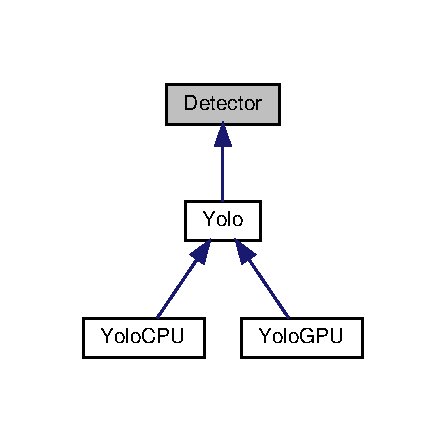
\includegraphics[width=214pt]{class_detector__inherit__graph}
\end{center}
\end{figure}
\subsection*{Public Member Functions}
\begin{DoxyCompactItemize}
\item 
\mbox{\label{class_detector_a608942d93773419f166a499be33bb7c1}} 
virtual std\+::vector$<$ \textbf{ Detected\+Object} $>$ {\bfseries find\+Objects} (cv\+::\+Mat color, cv\+::\+Mat depth)
\end{DoxyCompactItemize}


The documentation for this class was generated from the following file\+:\begin{DoxyCompactItemize}
\item 
model/reco\+Activite/reco\+Image/Detector.\+h\end{DoxyCompactItemize}

\section{selective\+Depth\+:\+:edge Struct Reference}
\label{structselective_depth_1_1edge}\index{selective\+Depth\+::edge@{selective\+Depth\+::edge}}
\subsection*{Public Attributes}
\begin{DoxyCompactItemize}
\item 
\mbox{\label{structselective_depth_1_1edge_ab45be8e09e44fa7757805524f0603235}} 
int {\bfseries a}
\item 
\mbox{\label{structselective_depth_1_1edge_a156de118dc10a5d81c9783c42b9ff76b}} 
int {\bfseries b}
\item 
\mbox{\label{structselective_depth_1_1edge_a1c6abe5af206afd831d5654c232c21b0}} 
double {\bfseries w}
\end{DoxyCompactItemize}


The documentation for this struct was generated from the following file\+:\begin{DoxyCompactItemize}
\item 
model/reco\+Activite/reco\+Image/selective\+Search\+Depth.\+h\end{DoxyCompactItemize}

\section{extended\+Plan\+Library Class Reference}
\label{classextended_plan_library}\index{extended\+Plan\+Library@{extended\+Plan\+Library}}


Collaboration diagram for extended\+Plan\+Library\+:
\nopagebreak
\begin{figure}[H]
\begin{center}
\leavevmode
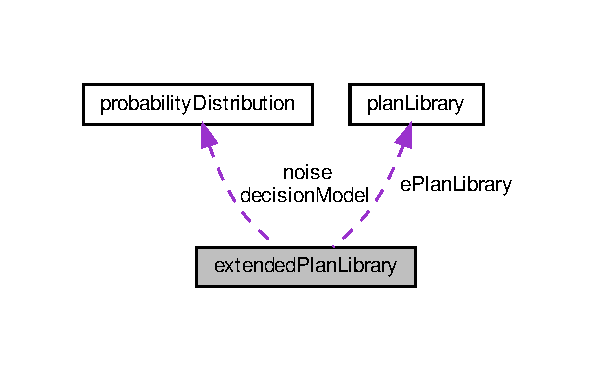
\includegraphics[width=287pt]{classextended_plan_library__coll__graph}
\end{center}
\end{figure}
\subsection*{Public Member Functions}
\begin{DoxyCompactItemize}
\item 
\mbox{\label{classextended_plan_library_ab11fbde77535d6bc627ec3df451c3f11}} 
{\bfseries extended\+Plan\+Library} (const char $\ast$spl)
\item 
\mbox{\label{classextended_plan_library_a0d19981e96203b01bf6707bef31b9f34}} 
{\bfseries extended\+Plan\+Library} (\textbf{ plan\+Library} $\ast$\+\_\+e\+Plan\+Library)
\item 
\mbox{\label{classextended_plan_library_a70a6870f3d6a25c5d42668f384c9493d}} 
{\bfseries extended\+Plan\+Library} (const \textbf{ extended\+Plan\+Library} \&epl)
\item 
\mbox{\label{classextended_plan_library_a0d31668984ad5bc8e7c0993cf0c45651}} 
{\bfseries extended\+Plan\+Library} (bool rnd=true, float noise\+P\+R\+CT=0.\+0, int goal=5, int \+\_\+size=10, int depth=2, int width\+A\+ND=3, int width\+OR=2, bool DM=false)
\item 
\mbox{\label{classextended_plan_library_a804ea71b83f1c288d6beab0caad7fec3}} 
int {\bfseries extra} ()
\item 
\mbox{\label{classextended_plan_library_ab28011e80bd6b2bdbd5dbeb0ad0852c4}} 
const string {\bfseries to\+String} ()
\end{DoxyCompactItemize}
\subsection*{Public Attributes}
\begin{DoxyCompactItemize}
\item 
\mbox{\label{classextended_plan_library_adfdeadb3a9690edfca909654225be623}} 
\textbf{ plan\+Library} $\ast$ {\bfseries e\+Plan\+Library}
\item 
\mbox{\label{classextended_plan_library_a1101073d7204ead7bc74adc82a60883b}} 
\textbf{ probability\+Distribution} {\bfseries decision\+Model}
\item 
\mbox{\label{classextended_plan_library_a912a4990ef0413b38d12db23216297b6}} 
\textbf{ probability\+Distribution} {\bfseries noise}
\item 
\mbox{\label{classextended_plan_library_a2bcd4077b34545e5dba7d988ec299eca}} 
map$<$ string, int $>$ {\bfseries ids}
\item 
\mbox{\label{classextended_plan_library_a57548009a05ac7723e2fab4df9212eee}} 
map$<$ int, string $>$ {\bfseries rev\+Ids}
\end{DoxyCompactItemize}


The documentation for this class was generated from the following files\+:\begin{DoxyCompactItemize}
\item 
model/reco\+Plan/\+P\+A\+R\+C/include/extended\+Plan\+Library.\+h\item 
model/reco\+Plan/\+P\+A\+R\+C/\+Plan\+\_\+\+Library/extended\+Plan\+Library.\+cpp\end{DoxyCompactItemize}

\section{std\+:\+:hash$<$ rule $>$ Struct Template Reference}
\label{structstd_1_1hash_3_01rule_01_4}\index{std\+::hash$<$ rule $>$@{std\+::hash$<$ rule $>$}}
\subsection*{Public Member Functions}
\begin{DoxyCompactItemize}
\item 
\mbox{\label{structstd_1_1hash_3_01rule_01_4_a840ba7e533dcc8b1e8e9848659b496f6}} 
size\+\_\+t {\bfseries operator()} (const \textbf{ rule} \&obj) const
\end{DoxyCompactItemize}


The documentation for this struct was generated from the following file\+:\begin{DoxyCompactItemize}
\item 
model/reco\+Plan/\+P\+A\+R\+C/include/rule.\+h\end{DoxyCompactItemize}

\section{std\+:\+:hash$<$ std\+:\+:pair$<$ int, int $>$ $>$ Class Template Reference}
\label{classstd_1_1hash_3_01std_1_1pair_3_01int_00_01int_01_4_01_4}\index{std\+::hash$<$ std\+::pair$<$ int, int $>$ $>$@{std\+::hash$<$ std\+::pair$<$ int, int $>$ $>$}}
\subsection*{Public Member Functions}
\begin{DoxyCompactItemize}
\item 
\mbox{\label{classstd_1_1hash_3_01std_1_1pair_3_01int_00_01int_01_4_01_4_ac8aa39f44d328e408d62466330d10df3}} 
std\+::size\+\_\+t {\bfseries operator()} (const std\+::pair$<$ int, int $>$ \&x) const
\end{DoxyCompactItemize}


The documentation for this class was generated from the following file\+:\begin{DoxyCompactItemize}
\item 
model/reco\+Activite/reco\+Image/selective\+Search\+Depth.\+h\end{DoxyCompactItemize}

\section{bnf\+:\+:Interface$<$ Data $>$ Struct Template Reference}
\label{structbnf_1_1_interface}\index{bnf\+::\+Interface$<$ Data $>$@{bnf\+::\+Interface$<$ Data $>$}}
\subsection*{Public Member Functions}
\begin{DoxyCompactItemize}
\item 
\mbox{\label{structbnf_1_1_interface_a3ba100a5958043abd670dee6ef03f270}} 
{\bfseries Interface} (const \textbf{ Interface} \&ifc, const char $\ast$text, size\+\_\+t length, const char $\ast$name)
\item 
\mbox{\label{structbnf_1_1_interface_ad1e1e4c8bb31ff77f9d4788c79474aec}} 
{\bfseries Interface} (const char $\ast$text, size\+\_\+t length, const char $\ast$name)
\item 
\mbox{\label{structbnf_1_1_interface_a236a916bae10e78128bc491b098b4d14}} 
{\bfseries Interface} (Data data, std\+::vector$<$ \textbf{ Interface} $>$ \&res, const char $\ast$name=\char`\"{}\char`\"{})
\item 
\mbox{\label{structbnf_1_1_interface_a170e2e3bcecc0ba84db1c3f38c52e146}} 
{\bfseries Interface} (const \textbf{ Interface} \&front, const \textbf{ Interface} \&back, const char $\ast$name=\char`\"{}\char`\"{})
\item 
\mbox{\label{structbnf_1_1_interface_af5eb2a2b7f6f30b45a1de94a9c611914}} 
int {\bfseries \+\_\+get\+\_\+pstop} (const char $\ast$$\ast$pstop)
\end{DoxyCompactItemize}
\subsection*{Static Public Member Functions}
\begin{DoxyCompactItemize}
\item 
\mbox{\label{structbnf_1_1_interface_ace4d9c561d2dd98ab3c4adbc7649596a}} 
static \textbf{ Interface} {\bfseries By\+Pass} (std\+::vector$<$ \textbf{ Interface} $>$ \&res)
\end{DoxyCompactItemize}
\subsection*{Public Attributes}
\begin{DoxyCompactItemize}
\item 
\mbox{\label{structbnf_1_1_interface_aa58c913cebaaea8dfde2955386358b00}} 
Data {\bfseries data}
\item 
\mbox{\label{structbnf_1_1_interface_ac72ee5bc4b029637854bcb6589b8485b}} 
const char $\ast$ {\bfseries text}
\item 
\mbox{\label{structbnf_1_1_interface_af60c723b2583fd7be6bfd39c95db44fa}} 
size\+\_\+t {\bfseries length}
\item 
\mbox{\label{structbnf_1_1_interface_ad1692efc0dca5a71a0a2c1b417d22459}} 
const char $\ast$ {\bfseries name}
\end{DoxyCompactItemize}


The documentation for this struct was generated from the following file\+:\begin{DoxyCompactItemize}
\item 
model/reco\+Plan/\+P\+A\+R\+C/include/bnflite.\+h\end{DoxyCompactItemize}

\section{Kinect Class Reference}
\label{class_kinect}\index{Kinect@{Kinect}}


Inheritance diagram for Kinect\+:
\nopagebreak
\begin{figure}[H]
\begin{center}
\leavevmode
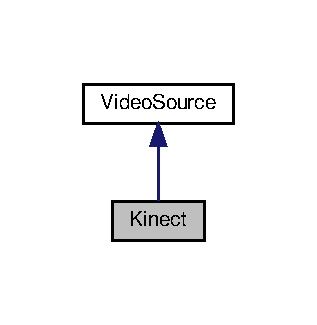
\includegraphics[width=152pt]{class_kinect__inherit__graph}
\end{center}
\end{figure}


Collaboration diagram for Kinect\+:
\nopagebreak
\begin{figure}[H]
\begin{center}
\leavevmode
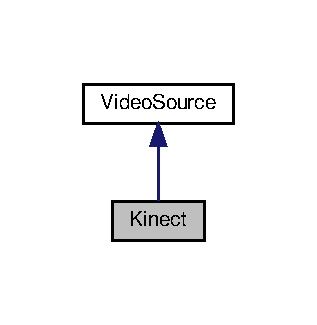
\includegraphics[width=152pt]{class_kinect__coll__graph}
\end{center}
\end{figure}
\subsection*{Public Member Functions}
\begin{DoxyCompactItemize}
\item 
\mbox{\label{class_kinect_a006fb9582a33bbc026834d34850c598c}} 
cv\+::\+Mat {\bfseries get\+Color\+Feed} ()
\item 
\mbox{\label{class_kinect_a2bc9f0dfe1117b46d1eb3740440a3a17}} 
cv\+::\+Mat {\bfseries get\+Depth\+Feed} ()
\item 
\mbox{\label{class_kinect_a0fab505f071a67d74b5124b1b8ef4fa1}} 
cv\+::\+Mat {\bfseries get\+Mapped\+Feed} ()
\item 
\mbox{\label{class_kinect_a8ff1afb85ee20e7bab9de5e13c3a9575}} 
cv\+::\+Mat {\bfseries get\+Original\+Depth} ()
\item 
\mbox{\label{class_kinect_a4b5ae8c02d4bfacff8a23fe2902da4b5}} 
void {\bfseries update} ()
\item 
\mbox{\label{class_kinect_abd18c649734b641a762fe33ec1df5836}} 
bool {\bfseries has\+Depth\+Source} ()
\item 
\mbox{\label{class_kinect_a3ed4b60fa61c3d5061a959d6b49b0851}} 
std\+::string {\bfseries get\+Time\+Stamp} ()
\item 
\mbox{\label{class_kinect_a1181d62f878e3eb681e76e7d8b7300f5}} 
int {\bfseries get\+Time\+Position} ()
\item 
\mbox{\label{class_kinect_a2588ce6e74cf51ffaa3fe3829042dff2}} 
double {\bfseries get\+Exact\+Time\+Position} ()
\item 
\mbox{\label{class_kinect_a39e9733b24bf29059fc36fbd7accc24c}} 
std\+::pair$<$ int, int $>$ {\bfseries get\+Screen\+Size} ()
\item 
\mbox{\label{class_kinect_a895813d18b5feb49ec0aa5358d3479df}} 
void {\bfseries acquire} ()
\item 
\mbox{\label{class_kinect_ab7736670c3d00426cb9ea12691eeb27f}} 
void {\bfseries release} ()
\end{DoxyCompactItemize}


The documentation for this class was generated from the following files\+:\begin{DoxyCompactItemize}
\item 
controller/sources/Kinect.\+h\item 
controller/sources/Kinect.\+cpp\end{DoxyCompactItemize}

\section{bnf\+:\+:Lexem Class Reference}
\label{classbnf_1_1_lexem}\index{bnf\+::\+Lexem@{bnf\+::\+Lexem}}


Inheritance diagram for bnf\+:\+:Lexem\+:
\nopagebreak
\begin{figure}[H]
\begin{center}
\leavevmode
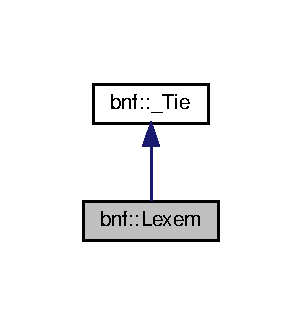
\includegraphics[width=145pt]{classbnf_1_1_lexem__inherit__graph}
\end{center}
\end{figure}


Collaboration diagram for bnf\+:\+:Lexem\+:
\nopagebreak
\begin{figure}[H]
\begin{center}
\leavevmode
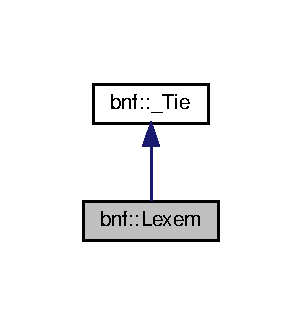
\includegraphics[width=145pt]{classbnf_1_1_lexem__coll__graph}
\end{center}
\end{figure}
\subsection*{Public Member Functions}
\begin{DoxyCompactItemize}
\item 
\mbox{\label{classbnf_1_1_lexem_a6001a7f84ee1921163fde124d26cb041}} 
{\bfseries Lexem} (const char $\ast$literal, bool cs=0)
\item 
\mbox{\label{classbnf_1_1_lexem_a1fadc96def543467f41dc371adbfad06}} 
{\bfseries Lexem} (const \textbf{ \+\_\+\+Tie} \&link)
\item 
\mbox{\label{classbnf_1_1_lexem_afd4583e3492fddeea0d9a53914a976f9}} 
\textbf{ Lexem} \& {\bfseries operator=} (const \textbf{ Lexem} \&lexem)
\item 
\mbox{\label{classbnf_1_1_lexem_a06fead13730b94041d9487c707bbbd4e}} 
\textbf{ Lexem} \& {\bfseries operator=} (const \textbf{ \+\_\+\+Tie} \&link)
\end{DoxyCompactItemize}
\subsection*{Protected Member Functions}
\begin{DoxyCompactItemize}
\item 
\mbox{\label{classbnf_1_1_lexem_adc34732c5794c9dc0e7287b215d1aefb}} 
{\bfseries Lexem} (\textbf{ Lexem} $\ast$lxm)
\item 
\mbox{\label{classbnf_1_1_lexem_ad8d44651fcf8e326d3064f76392fa4fd}} 
virtual int {\bfseries \+\_\+parse} (\textbf{ \+\_\+\+Base} $\ast$parser) const  throw ()
\end{DoxyCompactItemize}
\subsection*{Friends}
\begin{DoxyCompactItemize}
\item 
\mbox{\label{classbnf_1_1_lexem_ab555bd08f573aad86ad95feb76007c15}} 
class {\bfseries \+\_\+\+Tie}
\end{DoxyCompactItemize}
\subsection*{Additional Inherited Members}


The documentation for this class was generated from the following file\+:\begin{DoxyCompactItemize}
\item 
model/reco\+Plan/\+P\+A\+R\+C/include/bnflite.\+h\end{DoxyCompactItemize}

\section{Manage\+Source\+Video Class Reference}
\label{class_manage_source_video}\index{Manage\+Source\+Video@{Manage\+Source\+Video}}


Inheritance diagram for Manage\+Source\+Video\+:
\nopagebreak
\begin{figure}[H]
\begin{center}
\leavevmode
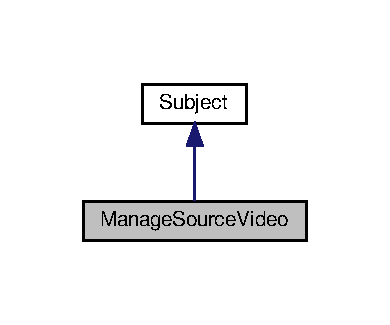
\includegraphics[width=187pt]{class_manage_source_video__inherit__graph}
\end{center}
\end{figure}


Collaboration diagram for Manage\+Source\+Video\+:
\nopagebreak
\begin{figure}[H]
\begin{center}
\leavevmode
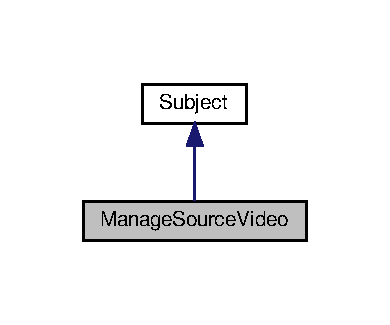
\includegraphics[width=187pt]{class_manage_source_video__coll__graph}
\end{center}
\end{figure}
\subsection*{Public Member Functions}
\begin{DoxyCompactItemize}
\item 
\textbf{ Manage\+Source\+Video} (map$<$ string, string $>$ setting)
\begin{DoxyCompactList}\small\item\em Constructor of class \doxyref{Manage\+Source\+Video}{p.}{class_manage_source_video}. \end{DoxyCompactList}\item 
\mbox{\label{class_manage_source_video_abb3cbceed45f55e2974ab26b576c4855}} 
virtual \textbf{ $\sim$\+Manage\+Source\+Video} ()
\begin{DoxyCompactList}\small\item\em Destructor of class \doxyref{Manage\+Source\+Video}{p.}{class_manage_source_video}. \end{DoxyCompactList}\item 
\mbox{\label{class_manage_source_video_a8b09bcb16decf02fa4d15616cf8f4f72}} 
std\+::string {\bfseries get\+Time\+Stamp} ()
\item 
\mbox{\label{class_manage_source_video_a390ec99cffdddd8883b3cc5944f39e1f}} 
int {\bfseries get\+Time\+Position} ()
\item 
\mbox{\label{class_manage_source_video_aa89ee19a989a075c9a83174f08fb21e8}} 
void {\bfseries update} ()
\item 
\mbox{\label{class_manage_source_video_a2c5bbbc4be945c8c4bbfc055110c51dd}} 
void {\bfseries choose\+Input\+Video} (string type\+Input\+Video, int width, int height, string path\+Source\+Video, string path\+Source\+Video\+Depth)
\item 
\mbox{\label{class_manage_source_video_a9e06741cecf33127bb3d525e641c8886}} 
cv\+::\+Mat {\bfseries get\+Original\+Image} ()
\item 
\mbox{\label{class_manage_source_video_a917bdd64974a58c8ee83637f772bab5e}} 
cv\+::\+Mat {\bfseries get\+Current\+Image} ()
\item 
\mbox{\label{class_manage_source_video_a9c80e87b3f6dad8f9cddbf91afdaf207}} 
cv\+::\+Mat {\bfseries get\+Depth\+Image} ()
\item 
\mbox{\label{class_manage_source_video_a93f2104b868fc8b3e19f812becf8bab4}} 
std\+::pair$<$ int, int $>$ {\bfseries get\+Screen\+Size} () const
\item 
\mbox{\label{class_manage_source_video_a103709220e4fe8367a4e0c7e8bd1e3eb}} 
void {\bfseries save\+Videos} ()
\item 
void \textbf{ register\+Observer} (\textbf{ Observer} $\ast$observer) override
\item 
void \textbf{ remove\+Observer} (\textbf{ Observer} $\ast$observer) override
\item 
void \textbf{ notify\+Observers} () override
\end{DoxyCompactItemize}


\subsection{Constructor \& Destructor Documentation}
\mbox{\label{class_manage_source_video_abdd3c50b750d59e5c801483e8e038be4}} 
\index{Manage\+Source\+Video@{Manage\+Source\+Video}!Manage\+Source\+Video@{Manage\+Source\+Video}}
\index{Manage\+Source\+Video@{Manage\+Source\+Video}!Manage\+Source\+Video@{Manage\+Source\+Video}}
\subsubsection{Manage\+Source\+Video()}
{\footnotesize\ttfamily Manage\+Source\+Video\+::\+Manage\+Source\+Video (\begin{DoxyParamCaption}\item[{map$<$ string, string $>$}]{setting }\end{DoxyParamCaption})}



Constructor of class \doxyref{Manage\+Source\+Video}{p.}{class_manage_source_video}. 


\begin{DoxyParams}{Parameters}
{\em setting} & \+: map$<$string,string$>$$\ast$ which contain every path and information to use (fisrt String = name\+\_\+of\+\_\+information, second String = information) \\
\hline
\end{DoxyParams}


\subsection{Member Function Documentation}
\mbox{\label{class_manage_source_video_a199cb436b1ca354c8a3723a33b2dd8d8}} 
\index{Manage\+Source\+Video@{Manage\+Source\+Video}!notify\+Observers@{notify\+Observers}}
\index{notify\+Observers@{notify\+Observers}!Manage\+Source\+Video@{Manage\+Source\+Video}}
\subsubsection{notify\+Observers()}
{\footnotesize\ttfamily void Manage\+Source\+Video\+::notify\+Observers (\begin{DoxyParamCaption}{ }\end{DoxyParamCaption})\hspace{0.3cm}{\ttfamily [override]}, {\ttfamily [virtual]}}

Notify all the registered observers when a change happens 

Implements \textbf{ Subject} \doxyref{}{p.}{class_subject_adb3adcf5638dda8dbd4b1d4356d02453}.

\mbox{\label{class_manage_source_video_a15dea65edbe41f3f58279a3ed291fce9}} 
\index{Manage\+Source\+Video@{Manage\+Source\+Video}!register\+Observer@{register\+Observer}}
\index{register\+Observer@{register\+Observer}!Manage\+Source\+Video@{Manage\+Source\+Video}}
\subsubsection{register\+Observer()}
{\footnotesize\ttfamily void Manage\+Source\+Video\+::register\+Observer (\begin{DoxyParamCaption}\item[{\textbf{ Observer} $\ast$}]{observer }\end{DoxyParamCaption})\hspace{0.3cm}{\ttfamily [override]}, {\ttfamily [virtual]}}

Register an observer 
\begin{DoxyParams}{Parameters}
{\em observer} & the observer object to be registered \\
\hline
\end{DoxyParams}


Implements \textbf{ Subject} \doxyref{}{p.}{class_subject_ae3f8d320b19b7d0fe695a3b4e7660002}.

\mbox{\label{class_manage_source_video_a7b6316cf6df23315705d4eb9bc0e07ff}} 
\index{Manage\+Source\+Video@{Manage\+Source\+Video}!remove\+Observer@{remove\+Observer}}
\index{remove\+Observer@{remove\+Observer}!Manage\+Source\+Video@{Manage\+Source\+Video}}
\subsubsection{remove\+Observer()}
{\footnotesize\ttfamily void Manage\+Source\+Video\+::remove\+Observer (\begin{DoxyParamCaption}\item[{\textbf{ Observer} $\ast$}]{observer }\end{DoxyParamCaption})\hspace{0.3cm}{\ttfamily [override]}, {\ttfamily [virtual]}}

Unregister an observer 
\begin{DoxyParams}{Parameters}
{\em observer} & the observer object to be unregistered \\
\hline
\end{DoxyParams}


Implements \textbf{ Subject} \doxyref{}{p.}{class_subject_a86699df0364a9091d1887f344255e9ff}.



The documentation for this class was generated from the following files\+:\begin{DoxyCompactItemize}
\item 
controller/\textbf{ Manage\+Source\+Video.\+h}\item 
controller/Manage\+Source\+Video.\+cpp\end{DoxyCompactItemize}

\section{Matrice\+Affordance Class Reference}
\label{class_matrice_affordance}\index{Matrice\+Affordance@{Matrice\+Affordance}}
\subsection*{Public Member Functions}
\begin{DoxyCompactItemize}
\item 
\textbf{ Matrice\+Affordance} ()
\begin{DoxyCompactList}\small\item\em Constructor of \doxyref{Matrice\+Affordance}{p.}{class_matrice_affordance}. \end{DoxyCompactList}\item 
\mbox{\label{class_matrice_affordance_a940661edba2a036c235db4c69b925407}} 
void \textbf{ reset} ()
\begin{DoxyCompactList}\small\item\em removes all the elements from mat\+\_\+objects \end{DoxyCompactList}\item 
\mbox{\label{class_matrice_affordance_a198c11b0b8429bc9a5cc417e294ca496}} 
void {\bfseries instance} ()
\item 
void \textbf{ addnew\+Aff} (\textbf{ Affordance} $\ast$aff, bool remove\+Last\+Value)
\begin{DoxyCompactList}\small\item\em update vector of last aff \end{DoxyCompactList}\item 
void \textbf{ update} (std\+::vector$<$ \textbf{ Affordance\+Time} $\ast$$>$ objs, bool remove\+Last\+Value)
\begin{DoxyCompactList}\small\item\em add last \doxyref{Affordance\+Time}{p.}{class_affordance_time}(vector of \doxyref{Affordance}{p.}{class_affordance} = every affordance possible for one frame) and suppress the oldest one if time since the start is great enough \end{DoxyCompactList}\item 
double \textbf{ get\+Frequence} (string name)
\begin{DoxyCompactList}\small\item\em returns the frequence of the affordance with an object in the last images $\vert$ Never Used \end{DoxyCompactList}\item 
double \textbf{ prob\+Calculation} (string name, double prob\+\_\+object)
\begin{DoxyCompactList}\small\item\em Calculation of the average probability \+: weighted average. \end{DoxyCompactList}\item 
\mbox{\label{class_matrice_affordance_a30ec6965bc564f64fa4c21c70cb7bdc9}} 
bool {\bfseries more\+Than\+Aff\+Frame} (string nom\+\_\+aff, int that)
\item 
\mbox{\label{class_matrice_affordance_a6e87fc1af407ea5e08187d9a282fcffc}} 
std\+::vector$<$ std\+::vector$<$ \textbf{ Affordance\+Time} $\ast$ $>$ $>$ {\bfseries get\+\_\+affordances} () const
\item 
\mbox{\label{class_matrice_affordance_a59553d4970376643f93668045ffc6fe7}} 
std\+::vector$<$ \textbf{ Affordance} $\ast$ $>$ {\bfseries get\+\_\+\+Mat\+\_\+prec\+\_\+act} () const
\end{DoxyCompactItemize}
\subsection*{Static Public Member Functions}
\begin{DoxyCompactItemize}
\item 
static \textbf{ Affordance} $\ast$ \textbf{ update\+Affordance} (const std\+::stack$<$ \textbf{ Affordance\+Time} $\ast$$>$ matrice)
\begin{DoxyCompactList}\small\item\em from the stack of Affordance\+Time$\ast$ return the most likely affordance of the last frame \end{DoxyCompactList}\end{DoxyCompactItemize}


\subsection{Constructor \& Destructor Documentation}
\mbox{\label{class_matrice_affordance_aa3814661eb661cab07fdfc9001a1d427}} 
\index{Matrice\+Affordance@{Matrice\+Affordance}!Matrice\+Affordance@{Matrice\+Affordance}}
\index{Matrice\+Affordance@{Matrice\+Affordance}!Matrice\+Affordance@{Matrice\+Affordance}}
\subsubsection{Matrice\+Affordance()}
{\footnotesize\ttfamily Matrice\+Affordance\+::\+Matrice\+Affordance (\begin{DoxyParamCaption}{ }\end{DoxyParamCaption})\hspace{0.3cm}{\ttfamily [inline]}}



Constructor of \doxyref{Matrice\+Affordance}{p.}{class_matrice_affordance}. 

initializes mat\+\_\+objets, matrix of objects 

\subsection{Member Function Documentation}
\mbox{\label{class_matrice_affordance_aa115589d909a394b21237e77daad8bcb}} 
\index{Matrice\+Affordance@{Matrice\+Affordance}!addnew\+Aff@{addnew\+Aff}}
\index{addnew\+Aff@{addnew\+Aff}!Matrice\+Affordance@{Matrice\+Affordance}}
\subsubsection{addnew\+Aff()}
{\footnotesize\ttfamily Matrice\+Affordance\+::addnew\+Aff (\begin{DoxyParamCaption}\item[{\textbf{ Affordance} $\ast$}]{aff,  }\item[{bool}]{remove\+Last\+Value }\end{DoxyParamCaption})\hspace{0.3cm}{\ttfamily [inline]}}



update vector of last aff 


\begin{DoxyParams}{Parameters}
{\em \doxyref{Affordance}{p.}{class_affordance}} & aff \+: last affordance seen \\
\hline
{\em bool} & remove\+Last\+Value \+: indicates if the time since the start is great enough for start to delete the oldest vector of affordance \\
\hline
\end{DoxyParams}
\mbox{\label{class_matrice_affordance_ad2f6f6e0f926492a34707c723a8dd45c}} 
\index{Matrice\+Affordance@{Matrice\+Affordance}!get\+Frequence@{get\+Frequence}}
\index{get\+Frequence@{get\+Frequence}!Matrice\+Affordance@{Matrice\+Affordance}}
\subsubsection{get\+Frequence()}
{\footnotesize\ttfamily Matrice\+Affordance\+::get\+Frequence (\begin{DoxyParamCaption}\item[{string}]{name }\end{DoxyParamCaption})\hspace{0.3cm}{\ttfamily [inline]}}



returns the frequence of the affordance with an object in the last images $\vert$ Never Used 


\begin{DoxyParams}{Parameters}
{\em name} & \+: Name of the class of the object to check \\
\hline
\end{DoxyParams}
\begin{DoxyReturn}{Returns}
the frequence of the object in the last images and itself 
\end{DoxyReturn}
\mbox{\label{class_matrice_affordance_a8627ac21309fadc468b7f00941166043}} 
\index{Matrice\+Affordance@{Matrice\+Affordance}!prob\+Calculation@{prob\+Calculation}}
\index{prob\+Calculation@{prob\+Calculation}!Matrice\+Affordance@{Matrice\+Affordance}}
\subsubsection{prob\+Calculation()}
{\footnotesize\ttfamily Matrice\+Affordance\+::prob\+Calculation (\begin{DoxyParamCaption}\item[{string}]{name,  }\item[{double}]{prob\+\_\+object }\end{DoxyParamCaption})\hspace{0.3cm}{\ttfamily [inline]}}



Calculation of the average probability \+: weighted average. 

(prob\+\_\+of\+\_\+object + sum(for i=2 to n) of (i/n) $\ast$ prob\+\_\+same\+\_\+object\+\_\+affordance\+\_\+at\+\_\+i\+\_\+frame\+\_\+of\+\_\+vector )/ sum(for i=1 to n) of i/n 
\begin{DoxyParams}{Parameters}
{\em name} & \+: Name of the class of the object to check \\
\hline
{\em prob\+\_\+object} & \+: probabilty of image recognition of the object (probability written on the screen in tread\+Picture \\
\hline
\end{DoxyParams}
\begin{DoxyReturn}{Returns}
double \+: probabilty of the affordance 
\end{DoxyReturn}
\mbox{\label{class_matrice_affordance_a8c313fa68aa813a1b4e3f40521098774}} 
\index{Matrice\+Affordance@{Matrice\+Affordance}!update@{update}}
\index{update@{update}!Matrice\+Affordance@{Matrice\+Affordance}}
\subsubsection{update()}
{\footnotesize\ttfamily Matrice\+Affordance\+::update (\begin{DoxyParamCaption}\item[{std\+::vector$<$ \textbf{ Affordance\+Time} $\ast$$>$}]{objs,  }\item[{bool}]{remove\+Last\+Value }\end{DoxyParamCaption})\hspace{0.3cm}{\ttfamily [inline]}}



add last \doxyref{Affordance\+Time}{p.}{class_affordance_time}(vector of \doxyref{Affordance}{p.}{class_affordance} = every affordance possible for one frame) and suppress the oldest one if time since the start is great enough 


\begin{DoxyParams}{Parameters}
{\em std\+::vector$<$\+Affordance\+Time$\ast$$>$} & objs \+: \doxyref{Affordance\+Time}{p.}{class_affordance_time}(vector of \doxyref{Affordance}{p.}{class_affordance} = every affordance possible for one frame) \\
\hline
{\em bool} & remove\+Last\+Value \+: indicates if the time since the start is great enough for start to delete the oldest vector of affordance \\
\hline
\end{DoxyParams}
\mbox{\label{class_matrice_affordance_ac9892b6441386d2ad01347c14840df67}} 
\index{Matrice\+Affordance@{Matrice\+Affordance}!update\+Affordance@{update\+Affordance}}
\index{update\+Affordance@{update\+Affordance}!Matrice\+Affordance@{Matrice\+Affordance}}
\subsubsection{update\+Affordance()}
{\footnotesize\ttfamily Matrice\+Affordance\+::update\+Affordance (\begin{DoxyParamCaption}\item[{const std\+::stack$<$ \textbf{ Affordance\+Time} $\ast$$>$}]{matrice }\end{DoxyParamCaption})\hspace{0.3cm}{\ttfamily [inline]}, {\ttfamily [static]}}



from the stack of Affordance\+Time$\ast$ return the most likely affordance of the last frame 

with vector of each affordance order by probability for each frame 
\begin{DoxyParams}{Parameters}
{\em const} & std\+::stack$<$\+Affordance\+Time$\ast$$>$ matrice \+: vector/stack of vector of affordance\+Time (first \+: each frame, second \+: each possibility for this frame \\
\hline
\end{DoxyParams}


The documentation for this class was generated from the following file\+:\begin{DoxyCompactItemize}
\item 
model/reco\+Activite/reco\+Affordance/\textbf{ Matrice\+Affordance.\+h}\end{DoxyCompactItemize}

\section{Object\+Affordances Class Reference}
\label{class_object_affordances}\index{Object\+Affordances@{Object\+Affordances}}
\subsection*{Public Member Functions}
\begin{DoxyCompactItemize}
\item 
\textbf{ Object\+Affordances} (int number\+Classes=10)
\begin{DoxyCompactList}\small\item\em Constructor of \doxyref{Object\+Affordances}{p.}{class_object_affordances}. \end{DoxyCompactList}\item 
void \textbf{ clear\+Current\+Affordances} ()
\begin{DoxyCompactList}\small\item\em clears current affordances of the object \end{DoxyCompactList}\item 
std\+::vector$<$ \textbf{ Affordance\+Time} $\ast$ $>$ \textbf{ find\+Affordances} (\textbf{ Detected\+Objects} \&regions, \textbf{ Detected\+Objects} \&hands, \textbf{ Matrice\+Affordance} \&Objects\+Mat, bool remove\+Last\+Value)
\begin{DoxyCompactList}\small\item\em finds the affordances between the hands and the different objects \end{DoxyCompactList}\item 
std\+::vector$<$ \textbf{ Affordance\+Time} $\ast$ $>$ \textbf{ add\+Null} (\textbf{ Matrice\+Affordance} \&object\+Mat, bool remove\+Last\+Value)
\begin{DoxyCompactList}\small\item\em adds a null affordance if no hands and no objects are detected \end{DoxyCompactList}\item 
\mbox{\label{class_object_affordances_acc72750bd4f0a062af9ae5ae96eeda8f}} 
\textbf{ Affordance\+Time} {\bfseries get\+Object\+Affordance} (const std\+::string object)
\item 
\mbox{\label{class_object_affordances_ab8b3bb3d0d33186a100572ead48a5c46}} 
std\+::vector$<$ \textbf{ Affordance\+Time} $>$ {\bfseries get\+Affordances} ()
\end{DoxyCompactItemize}
\subsection*{Friends}
\begin{DoxyCompactItemize}
\item 
std\+::istream \& \textbf{ operator$>$$>$} (std\+::istream \&is, \textbf{ Object\+Affordances} \&objaff)
\begin{DoxyCompactList}\small\item\em operator $>$$>$ \end{DoxyCompactList}\end{DoxyCompactItemize}


\subsection{Constructor \& Destructor Documentation}
\mbox{\label{class_object_affordances_a5b542eef939819cd120bbe0a63b32182}} 
\index{Object\+Affordances@{Object\+Affordances}!Object\+Affordances@{Object\+Affordances}}
\index{Object\+Affordances@{Object\+Affordances}!Object\+Affordances@{Object\+Affordances}}
\subsubsection{Object\+Affordances()}
{\footnotesize\ttfamily Object\+Affordances\+::\+Object\+Affordances (\begin{DoxyParamCaption}\item[{int}]{number\+Classes = {\ttfamily 10} }\end{DoxyParamCaption})}



Constructor of \doxyref{Object\+Affordances}{p.}{class_object_affordances}. 

initializes num\+Classes with the given parameter, sets frame\+Count and nb\+Classes to 0, sets current\+Aff to false 
\begin{DoxyParams}{Parameters}
{\em int} & number\+Classes \\
\hline
\end{DoxyParams}


\subsection{Member Function Documentation}
\mbox{\label{class_object_affordances_a61c42ae31ceaac32ccfb86200b75a6a3}} 
\index{Object\+Affordances@{Object\+Affordances}!add\+Null@{add\+Null}}
\index{add\+Null@{add\+Null}!Object\+Affordances@{Object\+Affordances}}
\subsubsection{add\+Null()}
{\footnotesize\ttfamily Object\+Affordances\+::add\+Null (\begin{DoxyParamCaption}\item[{\textbf{ Matrice\+Affordance} \&}]{object\+Mat,  }\item[{bool}]{sup\+Atime }\end{DoxyParamCaption})}



adds a null affordance if no hands and no objects are detected 

Creates a null affordance, adds it to the vector of affordances current\+Affordances, updates object\+Mat with the updated vector of affordances and returns current\+Affordances 
\begin{DoxyParams}{Parameters}
{\em \doxyref{Matrice\+Affordance}{p.}{class_matrice_affordance}} & \&object\+Mat \+: object from the class Object\+Mat \\
\hline
{\em bool} & sup\+Atime \+: boolean, indicates if more than a certain time passed since the start of the video \\
\hline
\end{DoxyParams}
\mbox{\label{class_object_affordances_a9bd8059744b50263d97fde3409d7fde9}} 
\index{Object\+Affordances@{Object\+Affordances}!clear\+Current\+Affordances@{clear\+Current\+Affordances}}
\index{clear\+Current\+Affordances@{clear\+Current\+Affordances}!Object\+Affordances@{Object\+Affordances}}
\subsubsection{clear\+Current\+Affordances()}
{\footnotesize\ttfamily Object\+Affordances\+::clear\+Current\+Affordances (\begin{DoxyParamCaption}{ }\end{DoxyParamCaption})}



clears current affordances of the object 

calls the clear() method of affordances, sets frame\+Count to 0 \mbox{\label{class_object_affordances_af8acefd33e80ca5566171e9590fac2e5}} 
\index{Object\+Affordances@{Object\+Affordances}!find\+Affordances@{find\+Affordances}}
\index{find\+Affordances@{find\+Affordances}!Object\+Affordances@{Object\+Affordances}}
\subsubsection{find\+Affordances()}
{\footnotesize\ttfamily Object\+Affordances\+::find\+Affordances (\begin{DoxyParamCaption}\item[{\textbf{ Detected\+Objects} \&}]{regions,  }\item[{\textbf{ Detected\+Objects} \&}]{hands,  }\item[{\textbf{ Matrice\+Affordance} \&}]{Objects\+Mat,  }\item[{bool}]{remove\+Last\+Value }\end{DoxyParamCaption})}



finds the affordances between the hands and the different objects 

Compares the distance between each objects and the hands. If their are affordances, returnes the vector of \doxyref{Affordance\+Time}{p.}{class_affordance_time} 
\begin{DoxyParams}{Parameters}
{\em Detected\+Objects\&} & regions \+: object from the class \doxyref{Detected\+Objects}{p.}{class_detected_objects}, vector of objects detected on the screen besides Hands \\
\hline
{\em Detected\+Objects\&} & hands \+: object from the class \doxyref{Detected\+Objects}{p.}{class_detected_objects}, vector of hands detected on the screen \\
\hline
{\em Matrice\+Affordance\&} & Objects\+Mat \+: object having a vector of \doxyref{Affordance\+Time}{p.}{class_affordance_time} \\
\hline
{\em bool} & sup\+Atime \+: boolean, indicates if more than a certain time passed since the start of the video \\
\hline
\end{DoxyParams}


\subsection{Friends And Related Function Documentation}
\mbox{\label{class_object_affordances_aa3b4883534360440aa3e598a3da82eb0}} 
\index{Object\+Affordances@{Object\+Affordances}!operator$>$$>$@{operator$>$$>$}}
\index{operator$>$$>$@{operator$>$$>$}!Object\+Affordances@{Object\+Affordances}}
\subsubsection{operator$>$$>$}
{\footnotesize\ttfamily std\+::istream \& operator$>$$>$ (\begin{DoxyParamCaption}\item[{std\+::istream \&}]{is,  }\item[{\textbf{ Object\+Affordances} \&}]{objaff }\end{DoxyParamCaption})\hspace{0.3cm}{\ttfamily [friend]}}



operator $>$$>$ 


\begin{DoxyParams}{Parameters}
{\em is} & \\
\hline
{\em objaff} & \\
\hline
\end{DoxyParams}
\begin{DoxyReturn}{Returns}

\end{DoxyReturn}


The documentation for this class was generated from the following files\+:\begin{DoxyCompactItemize}
\item 
model/reco\+Activite/reco\+Affordance/\textbf{ Object\+Aff.\+h}\item 
model/reco\+Activite/reco\+Affordance/Object\+Aff.\+cpp\end{DoxyCompactItemize}

\section{Observer Class Reference}
\label{class_observer}\index{Observer@{Observer}}


{\ttfamily \#include $<$Observer.\+h$>$}



Inheritance diagram for Observer\+:
\nopagebreak
\begin{figure}[H]
\begin{center}
\leavevmode
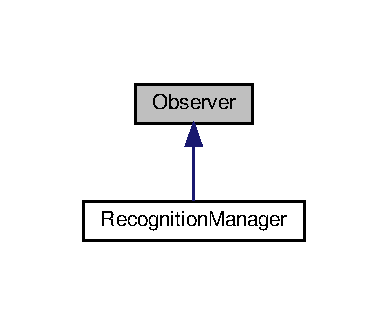
\includegraphics[width=186pt]{class_observer__inherit__graph}
\end{center}
\end{figure}
\subsection*{Public Member Functions}
\begin{DoxyCompactItemize}
\item 
virtual void \textbf{ update\+By\+Observee} (cv\+::\+Mat image\+Color, cv\+::\+Mat image\+Depth)=0
\end{DoxyCompactItemize}


\subsection{Detailed Description}
Interface for the \doxyref{Observer}{p.}{class_observer} 

\subsection{Member Function Documentation}
\mbox{\label{class_observer_a88fce56285a1da63ebc78300e4d5fcd4}} 
\index{Observer@{Observer}!update\+By\+Observee@{update\+By\+Observee}}
\index{update\+By\+Observee@{update\+By\+Observee}!Observer@{Observer}}
\subsubsection{update\+By\+Observee()}
{\footnotesize\ttfamily virtual void Observer\+::update\+By\+Observee (\begin{DoxyParamCaption}\item[{cv\+::\+Mat}]{image\+Color,  }\item[{cv\+::\+Mat}]{image\+Depth }\end{DoxyParamCaption})\hspace{0.3cm}{\ttfamily [pure virtual]}}

Update the state of this observer 
\begin{DoxyParams}{Parameters}
{\em test} & entier de test \\
\hline
\end{DoxyParams}


The documentation for this class was generated from the following file\+:\begin{DoxyCompactItemize}
\item 
model/Observer.\+h\end{DoxyCompactItemize}

\section{plan\+Library Class Reference}
\label{classplan_library}\index{plan\+Library@{plan\+Library}}
\subsection*{Public Member Functions}
\begin{DoxyCompactItemize}
\item 
\mbox{\label{classplan_library_ad32fd62936aacfd6a66ba0788789589c}} 
{\bfseries plan\+Library} (const \textbf{ plan\+Library} \&\+\_\+pl)
\item 
\mbox{\label{classplan_library_ac23c498458f325de21c20ea810ccf609}} 
{\bfseries plan\+Library} (const char $\ast$spl)
\item 
\mbox{\label{classplan_library_a6f995fa1200fb6ff4fcfe7e77d7e969d}} 
bool {\bfseries is\+Terminal} (int symbol) const
\item 
\mbox{\label{classplan_library_a10dd4ab4e6ac92771e14420682a8cc82}} 
bool {\bfseries is\+Goal} (int symbol) const
\item 
\mbox{\label{classplan_library_adde959ef183ee7f55d47792682383f6b}} 
int {\bfseries add\+Symbol} (int s, bool t, bool g)
\item 
\mbox{\label{classplan_library_af9e0b63486499c9025f5ad4e094f8c42}} 
int {\bfseries add\+Rule} (\textbf{ rule} r)
\item 
\mbox{\label{classplan_library_afd0d1ddca9bff437cf43d13ee6fa8a1b}} 
const string {\bfseries to\+String} ()
\item 
\mbox{\label{classplan_library_a09f0bcb6a4afe166e62e2a28f95d4562}} 
const unordered\+\_\+set$<$ int $>$ \& {\bfseries get\+Terminals} () const
\item 
\mbox{\label{classplan_library_ad60232fcae8cc2b5f9b4d10d25aca244}} 
const unordered\+\_\+set$<$ int $>$ \& {\bfseries get\+Non\+Terminals} () const
\item 
\mbox{\label{classplan_library_adc221719b20bbd5d3de332b11177de54}} 
const unordered\+\_\+set$<$ int $>$ \& {\bfseries get\+Goals} () const
\item 
\mbox{\label{classplan_library_aedd683affefeaac850d80183881f7103}} 
const unordered\+\_\+map$<$ int, \textbf{ rule} $>$ \& {\bfseries get\+Rules} () const
\end{DoxyCompactItemize}


The documentation for this class was generated from the following files\+:\begin{DoxyCompactItemize}
\item 
model/reco\+Plan/\+P\+A\+R\+C/include/\textbf{ plan\+Library.\+h}\item 
model/reco\+Plan/\+P\+A\+R\+C/\+Plan\+\_\+\+Library/plan\+Library.\+cpp\end{DoxyCompactItemize}

\section{Policy Class Reference}
\label{class_policy}\index{Policy@{Policy}}
\subsection*{Public Member Functions}
\begin{DoxyCompactItemize}
\item 
\mbox{\label{class_policy_a0a3f02e2e3b1e5ffc1296b7f3a66c755}} 
\textbf{ Policy} ()
\begin{DoxyCompactList}\small\item\em Constructor of \doxyref{Policy}{p.}{class_policy}. \end{DoxyCompactList}\item 
bool \textbf{ update} (\textbf{ Affordance} $\ast$observation)
\begin{DoxyCompactList}\small\item\em adds the current observation in gP \end{DoxyCompactList}\item 
\mbox{\label{class_policy_a424474d6fe98df78b29a25b892ff8253}} 
void \textbf{ Reset} ()
\begin{DoxyCompactList}\small\item\em gP becomes a new solver \end{DoxyCompactList}\item 
std\+::vector$<$ std\+::pair$<$ std\+::string, float $>$ $>$ \textbf{ get\+Next\+Actions} ()
\begin{DoxyCompactList}\small\item\em get\+Next\+Actions \end{DoxyCompactList}\item 
std\+::vector$<$ std\+::pair$<$ std\+::string, float $>$ $>$ \textbf{ get\+Goals\+Proba} ()
\begin{DoxyCompactList}\small\item\em get\+Goals\+Proba \end{DoxyCompactList}\item 
bool \textbf{ load} (string path\+Domain)
\end{DoxyCompactItemize}


\subsection{Member Function Documentation}
\mbox{\label{class_policy_aac733f255b894c3329d26d3a4f43e27d}} 
\index{Policy@{Policy}!get\+Goals\+Proba@{get\+Goals\+Proba}}
\index{get\+Goals\+Proba@{get\+Goals\+Proba}!Policy@{Policy}}
\subsubsection{get\+Goals\+Proba()}
{\footnotesize\ttfamily std\+::vector$<$ std\+::pair$<$ std\+::string, float $>$ $>$ Policy\+::get\+Goals\+Proba (\begin{DoxyParamCaption}{ }\end{DoxyParamCaption})}



get\+Goals\+Proba 

\begin{DoxyReturn}{Returns}

\end{DoxyReturn}
\mbox{\label{class_policy_a31a8e9b98126f1eced73813741813c30}} 
\index{Policy@{Policy}!get\+Next\+Actions@{get\+Next\+Actions}}
\index{get\+Next\+Actions@{get\+Next\+Actions}!Policy@{Policy}}
\subsubsection{get\+Next\+Actions()}
{\footnotesize\ttfamily std\+::vector$<$ std\+::pair$<$ std\+::string, float $>$ $>$ Policy\+::get\+Next\+Actions (\begin{DoxyParamCaption}{ }\end{DoxyParamCaption})}



get\+Next\+Actions 

\begin{DoxyReturn}{Returns}

\end{DoxyReturn}
\mbox{\label{class_policy_ac8d437da61da38bffe406c3e1cb281fd}} 
\index{Policy@{Policy}!load@{load}}
\index{load@{load}!Policy@{Policy}}
\subsubsection{load()}
{\footnotesize\ttfamily Policy\+::load (\begin{DoxyParamCaption}\item[{string}]{path\+Domain }\end{DoxyParamCaption})}


\begin{DoxyParams}{Parameters}
{\em path\+Domain} & \+: string =$>$ path to choose Domain \\
\hline
\end{DoxyParams}
\begin{DoxyReturn}{Returns}
boolean 
\end{DoxyReturn}
\mbox{\label{class_policy_a295b12845fb3f830ac9218e212222973}} 
\index{Policy@{Policy}!update@{update}}
\index{update@{update}!Policy@{Policy}}
\subsubsection{update()}
{\footnotesize\ttfamily Policy\+::update (\begin{DoxyParamCaption}\item[{\textbf{ Affordance} $\ast$}]{observation }\end{DoxyParamCaption})}



adds the current observation in gP 


\begin{DoxyParams}{Parameters}
{\em observation} & \+: Affordance$\ast$ observation \\
\hline
\end{DoxyParams}


The documentation for this class was generated from the following files\+:\begin{DoxyCompactItemize}
\item 
model/reco\+Plan/\textbf{ Policy.\+h}\item 
model/reco\+Plan/Policy.\+cpp\end{DoxyCompactItemize}

\section{Primary\+Window Class Reference}
\label{class_primary_window}\index{Primary\+Window@{Primary\+Window}}
\subsection*{Public Member Functions}
\begin{DoxyCompactItemize}
\item 
\textbf{ Primary\+Window} (bool display)
\begin{DoxyCompactList}\small\item\em Constructor. \end{DoxyCompactList}\item 
void \textbf{ update\+View} (\textbf{ Activity\+Region} $\ast$act, std\+::vector$<$ \textbf{ Affordance\+Time} $\ast$$>$ current\+Affordance)
\begin{DoxyCompactList}\small\item\em update View \end{DoxyCompactList}\item 
void \textbf{ treat\+Picture} (\textbf{ Activity\+Region} $\ast$act, std\+::vector$<$ \textbf{ Affordance\+Time} $\ast$$>$ current\+Affordance)
\begin{DoxyCompactList}\small\item\em draw rectangle over hands and \end{DoxyCompactList}\end{DoxyCompactItemize}


\subsection{Constructor \& Destructor Documentation}
\mbox{\label{class_primary_window_a8b841d6991616941a6a17abfa60df260}} 
\index{Primary\+Window@{Primary\+Window}!Primary\+Window@{Primary\+Window}}
\index{Primary\+Window@{Primary\+Window}!Primary\+Window@{Primary\+Window}}
\subsubsection{Primary\+Window()}
{\footnotesize\ttfamily Primary\+Window\+::\+Primary\+Window (\begin{DoxyParamCaption}\item[{bool}]{display }\end{DoxyParamCaption})}



Constructor. 

enable all composant only if display is true 
\begin{DoxyParams}{Parameters}
{\em display} & \+: send by configuration file $\vert$ without one display is ON \\
\hline
\end{DoxyParams}


\subsection{Member Function Documentation}
\mbox{\label{class_primary_window_a06bec221f7a0a1f205976a6e21a2f29d}} 
\index{Primary\+Window@{Primary\+Window}!treat\+Picture@{treat\+Picture}}
\index{treat\+Picture@{treat\+Picture}!Primary\+Window@{Primary\+Window}}
\subsubsection{treat\+Picture()}
{\footnotesize\ttfamily Primary\+Window\+::treat\+Picture (\begin{DoxyParamCaption}\item[{\textbf{ Activity\+Region} $\ast$}]{act,  }\item[{std\+::vector$<$ \textbf{ Affordance\+Time} $\ast$$>$}]{current\+Affordance }\end{DoxyParamCaption})}



draw rectangle over hands and 

called by update\+View 
\begin{DoxyParams}{Parameters}
{\em act} & \+: Object of \doxyref{Activity\+Region}{p.}{class_activity_region}\+: contains image\+Color, position of hands and objects \\
\hline
{\em current\+Affordance} & \+: vector of Object of \doxyref{Affordance\+Time}{p.}{class_affordance_time} contain position of hands and objects \\
\hline
\end{DoxyParams}
\mbox{\label{class_primary_window_a81d64431709d41e7f3e5583cc494e65a}} 
\index{Primary\+Window@{Primary\+Window}!update\+View@{update\+View}}
\index{update\+View@{update\+View}!Primary\+Window@{Primary\+Window}}
\subsubsection{update\+View()}
{\footnotesize\ttfamily Primary\+Window\+::update\+View (\begin{DoxyParamCaption}\item[{\textbf{ Activity\+Region} $\ast$}]{act,  }\item[{std\+::vector$<$ \textbf{ Affordance\+Time} $\ast$$>$}]{current\+Affordance }\end{DoxyParamCaption})}



update View 

called by \doxyref{Recognition\+Manager}{p.}{class_recognition_manager} at each course of the loop call treat\+Picture which draw rectangle over the initial picture 
\begin{DoxyParams}{Parameters}
{\em act} & \+: Object of \doxyref{Activity\+Region}{p.}{class_activity_region}\+: contains image\+Color, position of hands and objects \\
\hline
{\em current\+Affordance} & \+: vector of Object of \doxyref{Affordance\+Time}{p.}{class_affordance_time} contain position of hands and objects \\
\hline
\end{DoxyParams}


The documentation for this class was generated from the following files\+:\begin{DoxyCompactItemize}
\item 
view/\textbf{ Primary\+Window.\+h}\item 
view/Primary\+Window.\+cpp\end{DoxyCompactItemize}

\section{probability\+Distribution Class Reference}
\label{classprobability_distribution}\index{probability\+Distribution@{probability\+Distribution}}
\subsection*{Public Member Functions}
\begin{DoxyCompactItemize}
\item 
\mbox{\label{classprobability_distribution_a2a995499889b4264a99eb5d4c929c560}} 
{\bfseries probability\+Distribution} (unordered\+\_\+map$<$ int, unordered\+\_\+map$<$ int, float $>$$>$ \+\_\+distribution)
\item 
\mbox{\label{classprobability_distribution_a701b32e41142bc9f298e516e4e422be4}} 
{\bfseries probability\+Distribution} (\textbf{ plan\+Library} \&\+\_\+pl)
\item 
\mbox{\label{classprobability_distribution_a7b482f50162c74e33558e911fa1d0cda}} 
{\bfseries probability\+Distribution} (unordered\+\_\+set$<$ int $>$ \+\_\+terminals, float noise=0.\+0)
\item 
\mbox{\label{classprobability_distribution_a430d2970d87e8e928ae00cb346d5400a}} 
bool {\bfseries is\+Valid} () const
\item 
\mbox{\label{classprobability_distribution_a08eb703110c0c00ec2425e23311446c9}} 
int {\bfseries R\+NC} (int i) const
\item 
\mbox{\label{classprobability_distribution_a760246a89973b3cdcb3e56716251530c}} 
void {\bfseries set\+Prob} (int primitive, int element, float probability)
\item 
\mbox{\label{classprobability_distribution_a09394253f3ca51cc426b4c666619003f}} 
void {\bfseries set\+Noise} (int Prct)
\item 
\mbox{\label{classprobability_distribution_a5cf179f2819de49f2d6524f4ff8efd35}} 
const unordered\+\_\+map$<$ int, unordered\+\_\+map$<$ int, float $>$ $>$ \& {\bfseries get\+Distribution} () const
\end{DoxyCompactItemize}


The documentation for this class was generated from the following files\+:\begin{DoxyCompactItemize}
\item 
model/reco\+Plan/\+P\+A\+R\+C/include/probability\+Distribution.\+h\item 
model/reco\+Plan/\+P\+A\+R\+C/\+Plan\+\_\+\+Library/probability\+Distribution.\+cpp\end{DoxyCompactItemize}

\section{Real\+Sense\+Video Class Reference}
\label{class_real_sense_video}\index{Real\+Sense\+Video@{Real\+Sense\+Video}}


Inheritance diagram for Real\+Sense\+Video\+:
\nopagebreak
\begin{figure}[H]
\begin{center}
\leavevmode
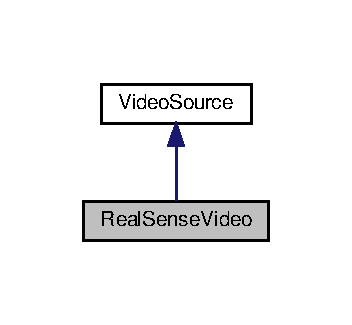
\includegraphics[width=169pt]{class_real_sense_video__inherit__graph}
\end{center}
\end{figure}


Collaboration diagram for Real\+Sense\+Video\+:
\nopagebreak
\begin{figure}[H]
\begin{center}
\leavevmode
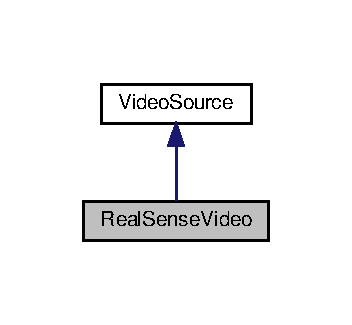
\includegraphics[width=169pt]{class_real_sense_video__coll__graph}
\end{center}
\end{figure}
\subsection*{Public Member Functions}
\begin{DoxyCompactItemize}
\item 
\mbox{\label{class_real_sense_video_a76e741fc745150c5d8b1dd7c0964d8ee}} 
{\bfseries Real\+Sense\+Video} (std\+::string color\+File=\char`\"{}\char`\"{}, std\+::string depth\+File=\char`\"{}\char`\"{})
\item 
\mbox{\label{class_real_sense_video_a59df1d401a21f7ec2a353bf5bac922dd}} 
cv\+::\+Mat {\bfseries get\+Color\+Feed} ()
\item 
\mbox{\label{class_real_sense_video_a59f27190cfe07d833752275e2181ca2a}} 
cv\+::\+Mat {\bfseries get\+Depth\+Feed} ()
\item 
\mbox{\label{class_real_sense_video_abb5ab3b64e7996e2af0f60157ca59423}} 
cv\+::\+Mat {\bfseries get\+Mapped\+Feed} ()
\item 
\mbox{\label{class_real_sense_video_af308dfa5dfaaca687c202d2c566739df}} 
cv\+::\+Mat {\bfseries get\+Original\+Depth} ()
\item 
\mbox{\label{class_real_sense_video_a18936f35d354d3fa5702b016018682d9}} 
void {\bfseries update} ()
\item 
\mbox{\label{class_real_sense_video_a82c9c5a3bc99df19cd0d26031f67d235}} 
bool {\bfseries has\+Depth\+Source} ()
\item 
\mbox{\label{class_real_sense_video_a116ba72253f5c99ea97b03b08d0d5152}} 
std\+::string {\bfseries get\+Time\+Stamp} ()
\item 
\mbox{\label{class_real_sense_video_a132141fd5d9fc85881606e29292dd141}} 
int {\bfseries get\+Time\+Position} ()
\item 
\mbox{\label{class_real_sense_video_add6fb9e7b923a848672767c2a6bef56b}} 
double {\bfseries get\+Exact\+Time\+Position} ()
\item 
\mbox{\label{class_real_sense_video_a3ac4729a8746898de82a373badb4ab69}} 
std\+::pair$<$ int, int $>$ {\bfseries get\+Screen\+Size} ()
\end{DoxyCompactItemize}


The documentation for this class was generated from the following files\+:\begin{DoxyCompactItemize}
\item 
controller/sources/Real\+Sense\+Video.\+h\item 
controller/sources/Real\+Sense\+Video.\+cpp\end{DoxyCompactItemize}

\section{Recognition\+Manager Class Reference}
\label{class_recognition_manager}\index{Recognition\+Manager@{Recognition\+Manager}}


Inheritance diagram for Recognition\+Manager\+:
\nopagebreak
\begin{figure}[H]
\begin{center}
\leavevmode
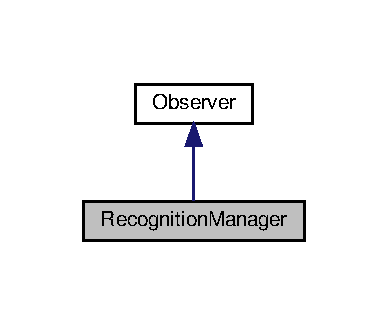
\includegraphics[width=186pt]{class_recognition_manager__inherit__graph}
\end{center}
\end{figure}


Collaboration diagram for Recognition\+Manager\+:
\nopagebreak
\begin{figure}[H]
\begin{center}
\leavevmode
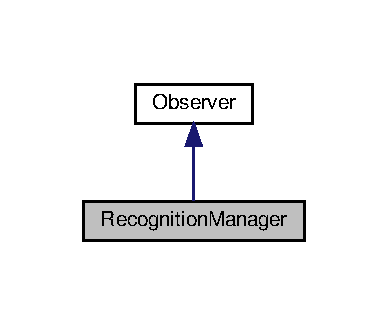
\includegraphics[width=186pt]{class_recognition_manager__coll__graph}
\end{center}
\end{figure}
\subsection*{Public Member Functions}
\begin{DoxyCompactItemize}
\item 
\textbf{ Recognition\+Manager} (\textbf{ Primary\+Window} $\ast$p\+\_\+view, \textbf{ Manage\+Source\+Video} $\ast$p\+\_\+controller, map$<$ string, string $>$ setting)
\begin{DoxyCompactList}\small\item\em Constructor. \end{DoxyCompactList}\item 
\mbox{\label{class_recognition_manager_af23137fcb979eadc69a872723fd5648c}} 
virtual \textbf{ $\sim$\+Recognition\+Manager} ()
\begin{DoxyCompactList}\small\item\em Destructor. \end{DoxyCompactList}\item 
void \textbf{ recognition\+Loop} (\textbf{ Manage\+Source\+Video} $\ast$p\+\_\+controller, \textbf{ Primary\+Window} $\ast$p\+\_\+view)
\begin{DoxyCompactList}\small\item\em main loop of recognition which update every composant of the program \end{DoxyCompactList}\item 
void \textbf{ update\+Intern\+Var} ()
\begin{DoxyCompactList}\small\item\em Update variable. \end{DoxyCompactList}\item 
void \textbf{ ask\+To\+Quit} ()
\begin{DoxyCompactList}\small\item\em Exit way (absolutly not necessary) $\vert$ Unused. \end{DoxyCompactList}\item 
void \textbf{ update\+By\+Observee} (Mat image\+Color, Mat image\+Depth)
\begin{DoxyCompactList}\small\item\em Called by Observee (Image\+Treatment) \end{DoxyCompactList}\item 
void \textbf{ update\+Affordance\+Seen} (\textbf{ Detected\+Objects} items, \textbf{ Detected\+Objects} hands, bool remove\+Last\+Value)
\begin{DoxyCompactList}\small\item\em With hands and objects position, and last affordances found the current one then check it. \end{DoxyCompactList}\item 
void \textbf{ update\+Plan\+Recognition} (\textbf{ Affordance} $\ast$checked\+Act\+Affordance)
\end{DoxyCompactItemize}


\subsection{Constructor \& Destructor Documentation}
\mbox{\label{class_recognition_manager_afd771fe50a86dc604338f5b47405357e}} 
\index{Recognition\+Manager@{Recognition\+Manager}!Recognition\+Manager@{Recognition\+Manager}}
\index{Recognition\+Manager@{Recognition\+Manager}!Recognition\+Manager@{Recognition\+Manager}}
\subsubsection{Recognition\+Manager()}
{\footnotesize\ttfamily Recognition\+Manager\+::\+Recognition\+Manager (\begin{DoxyParamCaption}\item[{\textbf{ Primary\+Window} $\ast$}]{p\+\_\+view,  }\item[{\textbf{ Manage\+Source\+Video} $\ast$}]{p\+\_\+controller,  }\item[{map$<$ string, string $>$}]{setting }\end{DoxyParamCaption})}



Constructor. 

Initialize reco\+Image, reco\+Activity and reco\+Plan 
\begin{DoxyParams}{Parameters}
{\em p\+\_\+controller} & \+: pointer on Object of \doxyref{Manage\+Source\+Video}{p.}{class_manage_source_video} created in \doxyref{main.\+cpp}{p.}{main_8cpp} \\
\hline
{\em p\+\_\+view} & \+: pointer on Object of Primary\+View created in \doxyref{main.\+cpp}{p.}{main_8cpp} \\
\hline
{\em setting} & \+: map$<$string,string$>$ which contain every path and information to use (fisrt String = name\+\_\+of\+\_\+information, second String = information) \\
\hline
\end{DoxyParams}
Add setting to his attribute

add this object as a listener of this object of Image\+Treatment

Initialize image recognition

Initialize activities/affordance recognition

Initialize plan recognition if path of Domain gived in config 

\subsection{Member Function Documentation}
\mbox{\label{class_recognition_manager_a4441f77ce8103c10fabe9a25a77fe799}} 
\index{Recognition\+Manager@{Recognition\+Manager}!ask\+To\+Quit@{ask\+To\+Quit}}
\index{ask\+To\+Quit@{ask\+To\+Quit}!Recognition\+Manager@{Recognition\+Manager}}
\subsubsection{ask\+To\+Quit()}
{\footnotesize\ttfamily Recognition\+Manager\+::ask\+To\+Quit (\begin{DoxyParamCaption}{ }\end{DoxyParamCaption})}



Exit way (absolutly not necessary) $\vert$ Unused. 

Ask if exit after T\+I\+M\+E\+\_\+\+B\+E\+F\+O\+R\+E\+\_\+\+A\+S\+K\+I\+N\+G\+\_\+\+C\+L\+O\+S\+U\+RE seconds $\vert$ U\+N\+U\+S\+ED.

not usefull and never call for now (we prefer let program run indefinitely) However \+: Could be useful in many ways (things which can be seen after the main loop) \mbox{\label{class_recognition_manager_a5dbeab3f91f5b2dc65e6f25589f3200c}} 
\index{Recognition\+Manager@{Recognition\+Manager}!recognition\+Loop@{recognition\+Loop}}
\index{recognition\+Loop@{recognition\+Loop}!Recognition\+Manager@{Recognition\+Manager}}
\subsubsection{recognition\+Loop()}
{\footnotesize\ttfamily Recognition\+Manager\+::recognition\+Loop (\begin{DoxyParamCaption}\item[{\textbf{ Manage\+Source\+Video} $\ast$}]{p\+\_\+controller,  }\item[{\textbf{ Primary\+Window} $\ast$}]{p\+\_\+view }\end{DoxyParamCaption})}



main loop of recognition which update every composant of the program 

take information(image) from controller then update model activities recognition return the affordance(\+When a hand interact with an object) then update recognition plan finally update view 
\begin{DoxyParams}{Parameters}
{\em p\+\_\+controller} & \+: adress of main object of controller to add this to listenner and ask for update \\
\hline
{\em p\+\_\+view} & \+: adress of main object of view to show to user \\
\hline
\end{DoxyParams}
Update variable and display information on console

Update input (Camera)

Update image recognition (send to Y\+O\+LO which update vectors of hands and objects)

Boolean which say if we start to remove the oldest frame keeped in memory

Update affordance recognition

Send information to View \+: O\+U\+T\+P\+UT

Ask if exit after T\+I\+M\+E\+\_\+\+B\+E\+F\+O\+R\+E\+\_\+\+A\+S\+K\+I\+N\+G\+\_\+\+C\+L\+O\+S\+U\+RE seconds \mbox{\label{class_recognition_manager_af82e3ed84598f8e4ff3c99e1f68ae25e}} 
\index{Recognition\+Manager@{Recognition\+Manager}!update\+Affordance\+Seen@{update\+Affordance\+Seen}}
\index{update\+Affordance\+Seen@{update\+Affordance\+Seen}!Recognition\+Manager@{Recognition\+Manager}}
\subsubsection{update\+Affordance\+Seen()}
{\footnotesize\ttfamily Recognition\+Manager\+::update\+Affordance\+Seen (\begin{DoxyParamCaption}\item[{\textbf{ Detected\+Objects}}]{items,  }\item[{\textbf{ Detected\+Objects}}]{hands,  }\item[{bool}]{remove\+Last\+Value }\end{DoxyParamCaption})}



With hands and objects position, and last affordances found the current one then check it. 

Update a vector of \doxyref{Affordance}{p.}{class_affordance} sort by their probability (\doxyref{Matrice\+Affordance}{p.}{class_matrice_affordance}) Could have an affordance with nothing If we don\textquotesingle{}t see any hands or objects only affordance is N\+U\+LL with 1 for probability Then in function to former image (T\+I\+M\+E\+\_\+\+L\+A\+S\+T\+\_\+\+A\+F\+F\+O\+R\+D\+A\+N\+CE) tell what is the most likely affordance Can say N\+U\+LL Then look on the average one Then check it 
\begin{DoxyParams}{Parameters}
{\em items} & \+: \doxyref{Detected\+Objects}{p.}{class_detected_objects} basically a vector of objects \\
\hline
{\em hands} & \+: \doxyref{Detected\+Objects}{p.}{class_detected_objects} basically a vector of hands \\
\hline
{\em remove\+Last\+Value} & \+: boolean which say if we have to remove the first affordance of the vector $\vert$ after T\+I\+M\+E\+\_\+\+L\+A\+S\+T\+\_\+\+A\+F\+F\+O\+R\+D\+A\+N\+CE we start to supress this one \\
\hline
\end{DoxyParams}
To see an affordance from each frame

check if aff not null and (doesn\textquotesingle{}t = the 2 before except if more than 5 sec ) and 3 time in last 0.\+8 s \mbox{\label{class_recognition_manager_a229cf0650eeeb6f218f8816f0bb76b46}} 
\index{Recognition\+Manager@{Recognition\+Manager}!update\+By\+Observee@{update\+By\+Observee}}
\index{update\+By\+Observee@{update\+By\+Observee}!Recognition\+Manager@{Recognition\+Manager}}
\subsubsection{update\+By\+Observee()}
{\footnotesize\ttfamily Recognition\+Manager\+::update\+By\+Observee (\begin{DoxyParamCaption}\item[{Mat}]{image\+Color,  }\item[{Mat}]{image\+Depth }\end{DoxyParamCaption})}



Called by Observee (Image\+Treatment) 

update color\+Matrix and Depth\+Matrix

belongs to \doxyref{Observer}{p.}{class_observer} routine (called by controller) T\+O\+DO \+: just past a pointer of an unconstant matrix because it\textquotesingle{}s use for see and modify 
\begin{DoxyParams}{Parameters}
{\em image\+Color} & \+: 3 matrix which represent R\+GB of the last image $\sim$ Not sure \\
\hline
{\em image\+Depth} & \+: a matrix which represent the depth of last image \\
\hline
\end{DoxyParams}
\mbox{\label{class_recognition_manager_a8c134aced9268cf0f9e184f387b64aeb}} 
\index{Recognition\+Manager@{Recognition\+Manager}!update\+Intern\+Var@{update\+Intern\+Var}}
\index{update\+Intern\+Var@{update\+Intern\+Var}!Recognition\+Manager@{Recognition\+Manager}}
\subsubsection{update\+Intern\+Var()}
{\footnotesize\ttfamily Recognition\+Manager\+::update\+Intern\+Var (\begin{DoxyParamCaption}{ }\end{DoxyParamCaption})}



Update variable. 

Update variable and display information on console. Update display and information each seconds \mbox{\label{class_recognition_manager_a4b2ae89b18760f1008530ed81205b5ec}} 
\index{Recognition\+Manager@{Recognition\+Manager}!update\+Plan\+Recognition@{update\+Plan\+Recognition}}
\index{update\+Plan\+Recognition@{update\+Plan\+Recognition}!Recognition\+Manager@{Recognition\+Manager}}
\subsubsection{update\+Plan\+Recognition()}
{\footnotesize\ttfamily void Recognition\+Manager\+::update\+Plan\+Recognition (\begin{DoxyParamCaption}\item[{\textbf{ Affordance} $\ast$}]{checked\+Act\+Affordance }\end{DoxyParamCaption})}

Update plan recognition 

The documentation for this class was generated from the following files\+:\begin{DoxyCompactItemize}
\item 
model/\textbf{ Recognition\+Manager.\+h}\item 
model/Recognition\+Manager.\+cpp\end{DoxyCompactItemize}

\section{selective\+Depth\+:\+:Region Struct Reference}
\label{structselective_depth_1_1_region}\index{selective\+Depth\+::\+Region@{selective\+Depth\+::\+Region}}
\subsection*{Public Member Functions}
\begin{DoxyCompactItemize}
\item 
\mbox{\label{structselective_depth_1_1_region_a5d659fccd0750c226b4fc63821ced175}} 
{\bfseries Region} (const cv\+::\+Rect \&rect, int label)
\item 
\mbox{\label{structselective_depth_1_1_region_aac63503bd4bb216501ea003277d83147}} 
{\bfseries Region} (const cv\+::\+Rect \&rect, int size, const std\+::vector$<$ float $>$ \&\&colour\+Hist, const std\+::vector$<$ float $>$ \&\&texture\+Hist, const std\+::vector$<$ float $>$ \&\&depth\+Hist, const std\+::vector$<$ int $>$ \&\&labels)
\item 
\mbox{\label{structselective_depth_1_1_region_aa8b1558d6089c3f1a4b57fef0f7b388e}} 
\textbf{ Region} \& {\bfseries operator=} (const \textbf{ Region} \&region)=default
\item 
\mbox{\label{structselective_depth_1_1_region_a77d71d191f85c9d85406531fd77278b8}} 
\textbf{ Region} \& {\bfseries operator=} (\textbf{ Region} \&\&region) noexcept
\item 
\mbox{\label{structselective_depth_1_1_region_ad51caeb8db9aaa3f1b4bc29190fbd4be}} 
{\bfseries Region} (\textbf{ Region} \&\&region) noexcept
\end{DoxyCompactItemize}
\subsection*{Public Attributes}
\begin{DoxyCompactItemize}
\item 
\mbox{\label{structselective_depth_1_1_region_a11936f5e3d03b380f1595f49420e39ed}} 
int {\bfseries size}
\item 
\mbox{\label{structselective_depth_1_1_region_acd1a7d83bb4732aa745f86717bdeb680}} 
cv\+::\+Rect {\bfseries rect}
\item 
\mbox{\label{structselective_depth_1_1_region_a1f2e7d85d30ddfb0a8705796ff2afaea}} 
std\+::vector$<$ int $>$ {\bfseries labels}
\item 
\mbox{\label{structselective_depth_1_1_region_a56fe4fb764ef369ef10559807663a4d8}} 
std\+::vector$<$ float $>$ {\bfseries colour\+Hist}
\item 
\mbox{\label{structselective_depth_1_1_region_a423f4dd693b66de386f4a7470c567557}} 
std\+::vector$<$ float $>$ {\bfseries depth\+Hist}
\item 
\mbox{\label{structselective_depth_1_1_region_a60db1050fdd57c5803c50405fdb3ea1d}} 
std\+::vector$<$ float $>$ {\bfseries texture\+Hist}
\end{DoxyCompactItemize}


The documentation for this struct was generated from the following file\+:\begin{DoxyCompactItemize}
\item 
model/reco\+Activite/reco\+Image/selective\+Search\+Depth.\+h\end{DoxyCompactItemize}

\section{bnf\+:\+:Rule Class Reference}
\label{classbnf_1_1_rule}\index{bnf\+::\+Rule@{bnf\+::\+Rule}}


Inheritance diagram for bnf\+:\+:Rule\+:
\nopagebreak
\begin{figure}[H]
\begin{center}
\leavevmode
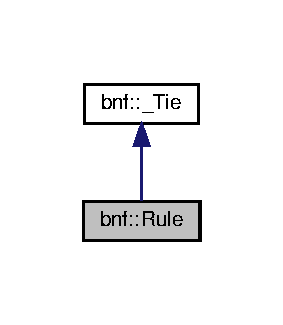
\includegraphics[width=136pt]{classbnf_1_1_rule__inherit__graph}
\end{center}
\end{figure}


Collaboration diagram for bnf\+:\+:Rule\+:
\nopagebreak
\begin{figure}[H]
\begin{center}
\leavevmode
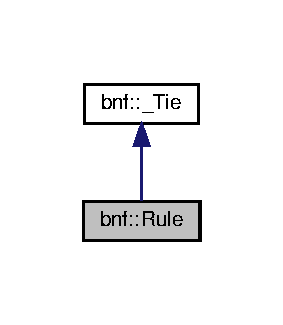
\includegraphics[width=136pt]{classbnf_1_1_rule__coll__graph}
\end{center}
\end{figure}
\subsection*{Public Member Functions}
\begin{DoxyCompactItemize}
\item 
\mbox{\label{classbnf_1_1_rule_a60dabd7f6981a64c258e7abd92d714a7}} 
{\bfseries Rule} (const \textbf{ \+\_\+\+Tie} \&link)
\item 
\mbox{\label{classbnf_1_1_rule_a67e1acace3996adffbbe39d98407d4fb}} 
\textbf{ Rule} \& {\bfseries operator=} (const \textbf{ \+\_\+\+Tie} \&link)
\item 
\mbox{\label{classbnf_1_1_rule_ae7b4e923d52fd9963747a0192d42e105}} 
\textbf{ Rule} \& {\bfseries operator=} (const \textbf{ Rule} \&\textbf{ rule})
\item 
\mbox{\label{classbnf_1_1_rule_a2c44184d509b95b5d6dc9bed966fe40e}} 
{\footnotesize template$<$class U $>$ }\\\textbf{ Rule} \& {\bfseries operator[$\,$]} (U($\ast$callback)(std\+::vector$<$ U $>$ \&))
\end{DoxyCompactItemize}
\subsection*{Protected Member Functions}
\begin{DoxyCompactItemize}
\item 
\mbox{\label{classbnf_1_1_rule_afa36b50741ac4b5bcc1e80effa6a2b55}} 
{\bfseries Rule} (const \textbf{ Rule} $\ast$rl)
\item 
\mbox{\label{classbnf_1_1_rule_a0460e1971d96c44b4885d7a72f5aec97}} 
virtual int {\bfseries \+\_\+parse} (\textbf{ \+\_\+\+Base} $\ast$parser) const  throw ()
\end{DoxyCompactItemize}
\subsection*{Friends}
\begin{DoxyCompactItemize}
\item 
\mbox{\label{classbnf_1_1_rule_ab555bd08f573aad86ad95feb76007c15}} 
class {\bfseries \+\_\+\+Tie}
\item 
\mbox{\label{classbnf_1_1_rule_abc37899b09eb024e8e57c00ec8fba682}} 
class {\bfseries \+\_\+\+And}
\item 
\mbox{\label{classbnf_1_1_rule_a3823850d893658658dfba4a9337b47e3}} 
{\footnotesize template$<$class U $>$ }\\\textbf{ Rule} \& {\bfseries Bind} (\textbf{ Rule} \&\textbf{ rule}, U($\ast$callback)(std\+::vector$<$ U $>$ \&))
\end{DoxyCompactItemize}
\subsection*{Additional Inherited Members}


The documentation for this class was generated from the following file\+:\begin{DoxyCompactItemize}
\item 
model/reco\+Plan/\+P\+A\+R\+C/include/bnflite.\+h\end{DoxyCompactItemize}

\section{rule Class Reference}
\label{classrule}\index{rule@{rule}}
\subsection*{Public Member Functions}
\begin{DoxyCompactItemize}
\item 
\mbox{\label{classrule_a57401587d56ba2964054d93c83b4fc91}} 
{\bfseries rule} (int \+\_\+primitive, int \+\_\+id)
\item 
\mbox{\label{classrule_a16818e659188b4f1178c0b79db6bad9e}} 
{\bfseries rule} (int \+\_\+id, string s)
\item 
\mbox{\label{classrule_a683407785d4a437670d3750de5a9443d}} 
void {\bfseries add\+Child} (int child)
\item 
\mbox{\label{classrule_a5a32df9cc88c5738753f5dab97ef0c78}} 
void {\bfseries add\+Constraint} (pair$<$ int, int $>$ constraint)
\item 
\mbox{\label{classrule_a254d66c82aa990b8aefbf1f455da4b54}} 
void {\bfseries add\+Children} (vector$<$ int $>$ \+\_\+children)
\item 
\mbox{\label{classrule_afc2f02214950cd290b778c7cdeed1dce}} 
void {\bfseries add\+Constraints} (vector$<$ pair$<$ int, int $>$$>$ \+\_\+constraints)
\item 
\mbox{\label{classrule_aa565618df29091d61d9c99dcae908c38}} 
bool {\bfseries operator$<$} (const \textbf{ rule} \+\_\+r) const
\item 
\mbox{\label{classrule_ad88299597acd5c12937f762887cc3123}} 
bool {\bfseries operator==} (const \textbf{ rule} \+\_\+r) const
\item 
\mbox{\label{classrule_a3583aea5924ca47331105829e7277c51}} 
{\bfseries operator int} () const
\item 
\mbox{\label{classrule_a69402285132b8065910c3a8e66c92ca0}} 
const int {\bfseries get\+Primitive} () const
\item 
\mbox{\label{classrule_a1affa4ca1a9b2d60e9b1e2ebd80af839}} 
const vector$<$ int $>$ \& {\bfseries get\+Children} () const
\item 
\mbox{\label{classrule_a0320b0278bbedf43ea858e5f4531cdc6}} 
const vector$<$ pair$<$ int, int $>$ $>$ \& {\bfseries get\+Constraints} () const
\item 
\mbox{\label{classrule_a7f67e512d14d0fb95d55dd819ec6a1cd}} 
const string {\bfseries to\+String} ()
\item 
\mbox{\label{classrule_ab13ae3fc714c9706d14ffdbcff0d2ccb}} 
const string {\bfseries to\+String} (map$<$ int, string $>$ rev\+Ids)
\end{DoxyCompactItemize}
\subsection*{Friends}
\begin{DoxyCompactItemize}
\item 
\mbox{\label{classrule_aaf5146e3508ab979d741cdada3c6e2b2}} 
std\+::ostream \& {\bfseries operator$<$$<$} (std\+::ostream \&, const \textbf{ rule} \&)
\end{DoxyCompactItemize}


The documentation for this class was generated from the following files\+:\begin{DoxyCompactItemize}
\item 
model/reco\+Plan/\+P\+A\+R\+C/include/rule.\+h\item 
model/reco\+Plan/\+P\+A\+R\+C/\+Plan\+\_\+\+Library/rule.\+cpp\end{DoxyCompactItemize}

\section{solver Class Reference}
\label{classsolver}\index{solver@{solver}}
\subsection*{Public Member Functions}
\begin{DoxyCompactItemize}
\item 
\mbox{\label{classsolver_a8ec9903435c8e17381aad968f0539003}} 
{\bfseries solver} (\textbf{ extended\+Plan\+Library} $\ast$\+\_\+epl, int \+\_\+nb\+Particle)
\item 
\mbox{\label{classsolver_ad3330e122355d5243387d0a92fc04978}} 
bool {\bfseries add\+Observation} (int obs)
\item 
\mbox{\label{classsolver_a041206bc0d3b165a141b24dfe8e0b90d}} 
bool {\bfseries add\+Observation} (std\+::string obs)
\item 
\mbox{\label{classsolver_a8eca9e760991959fc71913fd5987f886}} 
bool {\bfseries status} ()
\item 
\mbox{\label{classsolver_a18051200fe6815673e8a54822b726f97}} 
map$<$ int, int $>$ {\bfseries get\+Goals} ()
\item 
\mbox{\label{classsolver_ae1ba892ffdca41c210c34eadd84b19b5}} 
map$<$ int, int $>$ {\bfseries get\+Particles} ()
\item 
\mbox{\label{classsolver_a5f16741d3a28994464faa54280c98efa}} 
map$<$ std\+::string, float $>$ {\bfseries get\+Prob\+Goals} ()
\item 
\mbox{\label{classsolver_a93b69fb6a44494697a805d3b320c574c}} 
map$<$ std\+::string, float $>$ {\bfseries get\+Prob\+Particles} ()
\item 
\mbox{\label{classsolver_a96f03ffec3cba4c72fd83ae6ffd02f5c}} 
int {\bfseries get\+Max\+Goal} ()
\item 
\mbox{\label{classsolver_ace7514165a3e96c444392f53cd9b5ef4}} 
const int \& {\bfseries get\+Size} () const
\item 
\mbox{\label{classsolver_a10f3e831fbffb0ca926e3eedb840943e}} 
void {\bfseries clear} ()
\item 
\mbox{\label{classsolver_a7a4dcd1caf3438bc1a208aa3cb6ca2b2}} 
pair$<$ int, vector$<$ int $>$ $>$ {\bfseries generate\+Plan} ()
\item 
\mbox{\label{classsolver_a854e71f54847aa138ed08559873ad182}} 
pair$<$ int, vector$<$ int $>$ $>$ {\bfseries generate\+Plan\+FO} ()
\end{DoxyCompactItemize}


The documentation for this class was generated from the following files\+:\begin{DoxyCompactItemize}
\item 
model/reco\+Plan/\+P\+A\+R\+C/include/solver.\+h\item 
model/reco\+Plan/\+P\+A\+R\+C/src/solver/solver.\+cpp\end{DoxyCompactItemize}

\section{solver\+Particle Class Reference}
\label{classsolver_particle}\index{solver\+Particle@{solver\+Particle}}


Collaboration diagram for solver\+Particle\+:
\nopagebreak
\begin{figure}[H]
\begin{center}
\leavevmode
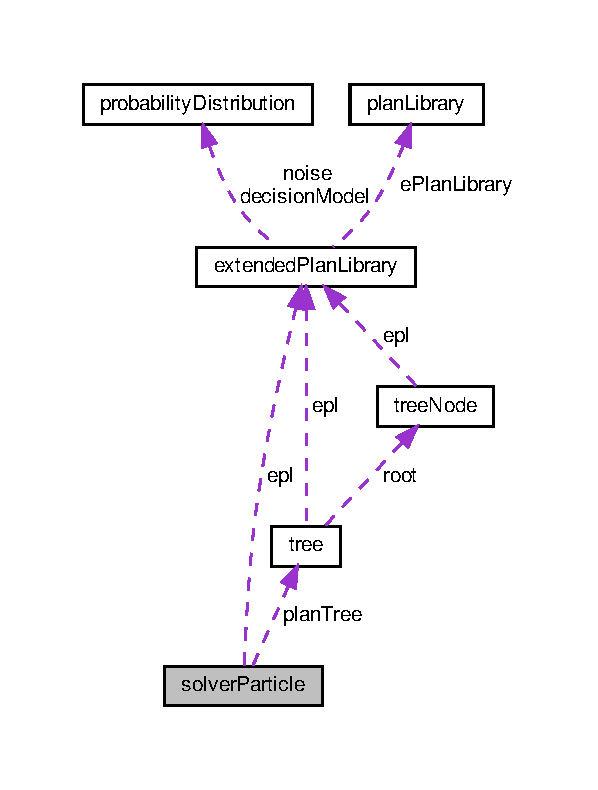
\includegraphics[width=287pt]{classsolver_particle__coll__graph}
\end{center}
\end{figure}
\subsection*{Public Member Functions}
\begin{DoxyCompactItemize}
\item 
\mbox{\label{classsolver_particle_a1a94b951cf5e503cf20b7df7a59428b0}} 
{\bfseries solver\+Particle} (\textbf{ extended\+Plan\+Library} $\ast$\+\_\+epl)
\item 
\mbox{\label{classsolver_particle_a036aa885efb5c6c4dbfa7a6840d4a68b}} 
bool {\bfseries update} ()
\end{DoxyCompactItemize}
\subsection*{Public Attributes}
\begin{DoxyCompactItemize}
\item 
\mbox{\label{classsolver_particle_a474cbf822017532e42fe641dd63370ef}} 
\textbf{ extended\+Plan\+Library} $\ast$ {\bfseries epl}
\item 
\mbox{\label{classsolver_particle_ac6455144f89db14fce27193d861066ab}} 
int {\bfseries goal}
\item 
\mbox{\label{classsolver_particle_a3fdf0c071a78a83ab49cc60cbc9a2d06}} 
vector$<$ int $>$ {\bfseries exp\+Next\+Obs}
\item 
\mbox{\label{classsolver_particle_a0e2950fe5ea4b71b686ae4986919327e}} 
\textbf{ tree} {\bfseries plan\+Tree}
\end{DoxyCompactItemize}


The documentation for this class was generated from the following files\+:\begin{DoxyCompactItemize}
\item 
model/reco\+Plan/\+P\+A\+R\+C/include/solver.\+h\item 
model/reco\+Plan/\+P\+A\+R\+C/src/solver/solver.\+cpp\end{DoxyCompactItemize}

\section{Subject Class Reference}
\label{class_subject}\index{Subject@{Subject}}


{\ttfamily \#include $<$Subject.\+h$>$}



Inheritance diagram for Subject\+:
\nopagebreak
\begin{figure}[H]
\begin{center}
\leavevmode
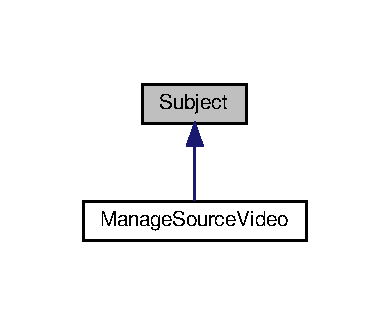
\includegraphics[width=187pt]{class_subject__inherit__graph}
\end{center}
\end{figure}
\subsection*{Public Member Functions}
\begin{DoxyCompactItemize}
\item 
virtual void \textbf{ register\+Observer} (\textbf{ Observer} $\ast$observer)=0
\item 
virtual void \textbf{ remove\+Observer} (\textbf{ Observer} $\ast$observer)=0
\item 
virtual void \textbf{ notify\+Observers} ()=0
\end{DoxyCompactItemize}


\subsection{Detailed Description}
Interface for the \doxyref{Subject}{p.}{class_subject} 

\subsection{Member Function Documentation}
\mbox{\label{class_subject_adb3adcf5638dda8dbd4b1d4356d02453}} 
\index{Subject@{Subject}!notify\+Observers@{notify\+Observers}}
\index{notify\+Observers@{notify\+Observers}!Subject@{Subject}}
\subsubsection{notify\+Observers()}
{\footnotesize\ttfamily virtual void Subject\+::notify\+Observers (\begin{DoxyParamCaption}{ }\end{DoxyParamCaption})\hspace{0.3cm}{\ttfamily [pure virtual]}}

Notify all the registered observers when a change happens 

Implemented in \textbf{ Manage\+Source\+Video} \doxyref{}{p.}{class_manage_source_video_a199cb436b1ca354c8a3723a33b2dd8d8}.

\mbox{\label{class_subject_ae3f8d320b19b7d0fe695a3b4e7660002}} 
\index{Subject@{Subject}!register\+Observer@{register\+Observer}}
\index{register\+Observer@{register\+Observer}!Subject@{Subject}}
\subsubsection{register\+Observer()}
{\footnotesize\ttfamily virtual void Subject\+::register\+Observer (\begin{DoxyParamCaption}\item[{\textbf{ Observer} $\ast$}]{observer }\end{DoxyParamCaption})\hspace{0.3cm}{\ttfamily [pure virtual]}}

Register an observer 
\begin{DoxyParams}{Parameters}
{\em observer} & the observer object to be registered \\
\hline
\end{DoxyParams}


Implemented in \textbf{ Manage\+Source\+Video} \doxyref{}{p.}{class_manage_source_video_a15dea65edbe41f3f58279a3ed291fce9}.

\mbox{\label{class_subject_a86699df0364a9091d1887f344255e9ff}} 
\index{Subject@{Subject}!remove\+Observer@{remove\+Observer}}
\index{remove\+Observer@{remove\+Observer}!Subject@{Subject}}
\subsubsection{remove\+Observer()}
{\footnotesize\ttfamily virtual void Subject\+::remove\+Observer (\begin{DoxyParamCaption}\item[{\textbf{ Observer} $\ast$}]{observer }\end{DoxyParamCaption})\hspace{0.3cm}{\ttfamily [pure virtual]}}

Unregister an observer 
\begin{DoxyParams}{Parameters}
{\em observer} & the observer object to be unregistered \\
\hline
\end{DoxyParams}


Implemented in \textbf{ Manage\+Source\+Video} \doxyref{}{p.}{class_manage_source_video_a7b6316cf6df23315705d4eb9bc0e07ff}.



The documentation for this class was generated from the following file\+:\begin{DoxyCompactItemize}
\item 
controller/Subject.\+h\end{DoxyCompactItemize}

\section{test\+Solver Class Reference}
\label{classtest_solver}\index{test\+Solver@{test\+Solver}}
\subsection*{Public Member Functions}
\begin{DoxyCompactItemize}
\item 
\mbox{\label{classtest_solver_a21b06892128ecd5ad11ec6bb6f4a5858}} 
{\bfseries test\+Solver} (int \+\_\+nb\+Test)
\item 
\mbox{\label{classtest_solver_aa9db0184fafc3f4ff962bfecdfb2d500}} 
void {\bfseries run} ()
\item 
\mbox{\label{classtest_solver_a9e0f0753e7d3a309da94fdb989046b3f}} 
void {\bfseries print} ()
\item 
\mbox{\label{classtest_solver_abb53fb745e83c43a7fb0bf0dba7310df}} 
void {\bfseries add\+Solver} (\textbf{ solver} s)
\end{DoxyCompactItemize}


The documentation for this class was generated from the following files\+:\begin{DoxyCompactItemize}
\item 
model/reco\+Plan/\+P\+A\+R\+C/include/test\+Solver.\+h\item 
model/reco\+Plan/\+P\+A\+R\+C/src/solver/test\+Solver.\+cpp\end{DoxyCompactItemize}

\section{bnf\+:\+:Token Class Reference}
\label{classbnf_1_1_token}\index{bnf\+::\+Token@{bnf\+::\+Token}}


Inheritance diagram for bnf\+:\+:Token\+:
\nopagebreak
\begin{figure}[H]
\begin{center}
\leavevmode
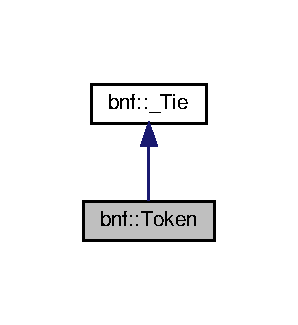
\includegraphics[width=143pt]{classbnf_1_1_token__inherit__graph}
\end{center}
\end{figure}


Collaboration diagram for bnf\+:\+:Token\+:
\nopagebreak
\begin{figure}[H]
\begin{center}
\leavevmode
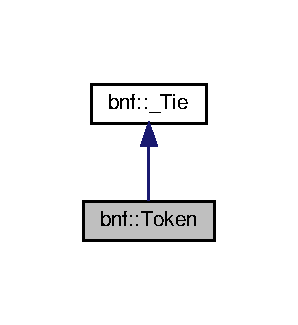
\includegraphics[width=143pt]{classbnf_1_1_token__coll__graph}
\end{center}
\end{figure}
\subsection*{Public Member Functions}
\begin{DoxyCompactItemize}
\item 
\mbox{\label{classbnf_1_1_token_aed0696c50a0fae76696157f108fbbc43}} 
{\bfseries Token} (const char c)
\item 
\mbox{\label{classbnf_1_1_token_aba69ea21ddea7965460bec26567ff11a}} 
{\bfseries Token} (int fst, int lst)
\item 
\mbox{\label{classbnf_1_1_token_a1a143d2e52f9e2f2ebf28fb23983b23e}} 
{\bfseries Token} (const char $\ast$s)
\item 
\mbox{\label{classbnf_1_1_token_aa2a87c84514305d23d686e76a13b531a}} 
{\bfseries Token} (const char $\ast$s, const \textbf{ Token} \&token)
\item 
\mbox{\label{classbnf_1_1_token_a80f5a655347bfd8719d5ed906fa8563f}} 
{\bfseries Token} (const \textbf{ Token} \&token)
\item 
\mbox{\label{classbnf_1_1_token_a1006b1383cd19db732176d9a2179f454}} 
void {\bfseries Add} (int fst, int lst=0)
\item 
\mbox{\label{classbnf_1_1_token_aebbe469ff4a8c576d136472758a68e1a}} 
void {\bfseries Add} (const char $\ast$sample)
\item 
\mbox{\label{classbnf_1_1_token_a5975313bf65e86a093bdd369b02f986e}} 
void {\bfseries Remove} (int fst, int lst=0)
\item 
\mbox{\label{classbnf_1_1_token_acbe7cc5ba1f6b22f16bfd6790510bba6}} 
void {\bfseries Remove} (const char $\ast$sample)
\item 
\mbox{\label{classbnf_1_1_token_afc1cc232799ef3977c968897a227a114}} 
int {\bfseries Get\+Symbol} (int next=0)
\item 
\mbox{\label{classbnf_1_1_token_a0e47888270947f053645d3571a72e39a}} 
\textbf{ Token} \& {\bfseries Invert} ()
\end{DoxyCompactItemize}
\subsection*{Protected Member Functions}
\begin{DoxyCompactItemize}
\item 
\mbox{\label{classbnf_1_1_token_af0f404eb33b567648857bc249b01d217}} 
{\bfseries Token} (const \textbf{ Token} $\ast$tkn)
\item 
\mbox{\label{classbnf_1_1_token_a94082cabb74558f2803657cae0a2ab44}} 
virtual int {\bfseries \+\_\+parse} (\textbf{ \+\_\+\+Base} $\ast$parser) const  throw ()
\end{DoxyCompactItemize}
\subsection*{Friends}
\begin{DoxyCompactItemize}
\item 
\mbox{\label{classbnf_1_1_token_ab555bd08f573aad86ad95feb76007c15}} 
class {\bfseries \+\_\+\+Tie}
\end{DoxyCompactItemize}
\subsection*{Additional Inherited Members}


The documentation for this class was generated from the following file\+:\begin{DoxyCompactItemize}
\item 
model/reco\+Plan/\+P\+A\+R\+C/include/bnflite.\+h\end{DoxyCompactItemize}

\section{tree Class Reference}
\label{classtree}\index{tree@{tree}}


Collaboration diagram for tree\+:
\nopagebreak
\begin{figure}[H]
\begin{center}
\leavevmode
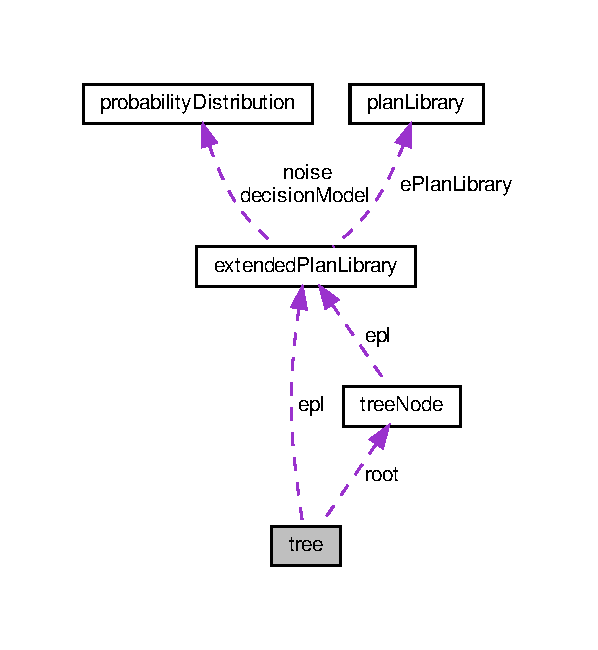
\includegraphics[width=287pt]{classtree__coll__graph}
\end{center}
\end{figure}
\subsection*{Public Member Functions}
\begin{DoxyCompactItemize}
\item 
\mbox{\label{classtree_a0ba809234501e7d0c9c5f97b178197c3}} 
{\bfseries tree} (\textbf{ extended\+Plan\+Library} $\ast$\+\_\+epl, int goal)
\item 
\mbox{\label{classtree_a3fada58a662386dbbb039eb106d35838}} 
vector$<$ int $>$ {\bfseries update} ()
\item 
\mbox{\label{classtree_af560bd89e9c3e894526a66c030dab3ea}} 
int {\bfseries update\+FO} ()
\end{DoxyCompactItemize}
\subsection*{Public Attributes}
\begin{DoxyCompactItemize}
\item 
\mbox{\label{classtree_a97066a8b966d6a0163696626f9ab2f16}} 
\textbf{ extended\+Plan\+Library} $\ast$ {\bfseries epl}
\item 
\mbox{\label{classtree_a268bedd9b37b4f6a09818cc612973d2d}} 
\textbf{ tree\+Node} {\bfseries root}
\end{DoxyCompactItemize}


The documentation for this class was generated from the following files\+:\begin{DoxyCompactItemize}
\item 
model/reco\+Plan/\+P\+A\+R\+C/include/solver.\+h\item 
model/reco\+Plan/\+P\+A\+R\+C/src/solver/solver.\+cpp\end{DoxyCompactItemize}

\section{tree\+Node Class Reference}
\label{classtree_node}\index{tree\+Node@{tree\+Node}}


Collaboration diagram for tree\+Node\+:
\nopagebreak
\begin{figure}[H]
\begin{center}
\leavevmode
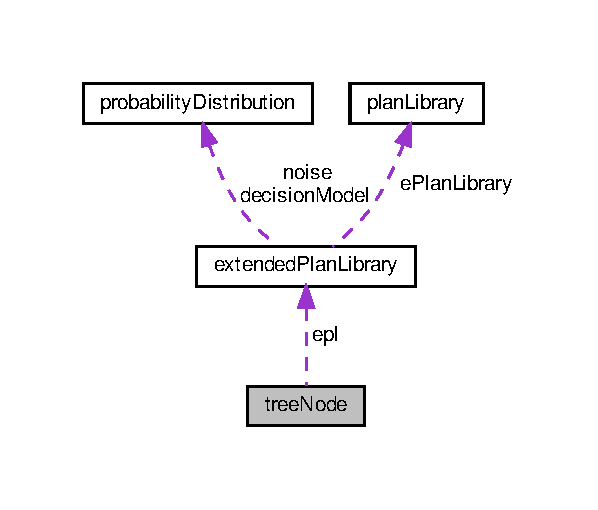
\includegraphics[width=287pt]{classtree_node__coll__graph}
\end{center}
\end{figure}
\subsection*{Public Member Functions}
\begin{DoxyCompactItemize}
\item 
\mbox{\label{classtree_node_abd735f769cfebe48e8503ddb7f0e8ef6}} 
{\bfseries tree\+Node} (\textbf{ extended\+Plan\+Library} $\ast$\+\_\+epl, int \+\_\+symbol)
\item 
\mbox{\label{classtree_node_a17b78ee258c263487eeafa8126817c82}} 
int {\bfseries update} ()
\end{DoxyCompactItemize}
\subsection*{Public Attributes}
\begin{DoxyCompactItemize}
\item 
\mbox{\label{classtree_node_a747fc45b98bbf29fd6832a7a32c717a0}} 
\textbf{ extended\+Plan\+Library} $\ast$ {\bfseries epl}
\item 
\mbox{\label{classtree_node_a84cfebe97cbef1ae4f1c6bfa110677ba}} 
int {\bfseries symbol}
\item 
\mbox{\label{classtree_node_ad9b561da695aed55e432e03680332b7c}} 
int {\bfseries \+\_\+rule}
\item 
\mbox{\label{classtree_node_a0a2564e246dd61e694d812e93629fa83}} 
bool {\bfseries status}
\item 
\mbox{\label{classtree_node_afc2f0e77a278b60136c983e019403b1b}} 
map$<$ int, \textbf{ tree\+Node} $>$ {\bfseries children}
\end{DoxyCompactItemize}


The documentation for this class was generated from the following files\+:\begin{DoxyCompactItemize}
\item 
model/reco\+Plan/\+P\+A\+R\+C/include/solver.\+h\item 
model/reco\+Plan/\+P\+A\+R\+C/src/solver/solver.\+cpp\end{DoxyCompactItemize}

\section{selective\+Depth\+:\+:Universe Class Reference}
\label{classselective_depth_1_1_universe}\index{selective\+Depth\+::\+Universe@{selective\+Depth\+::\+Universe}}
\subsection*{Public Member Functions}
\begin{DoxyCompactItemize}
\item 
\mbox{\label{classselective_depth_1_1_universe_a7557a2a93c9e2708366f317d46cd8e64}} 
{\bfseries Universe} (int num)
\item 
\mbox{\label{classselective_depth_1_1_universe_a3b22248be73dccc078ecf00c7d5d283e}} 
int {\bfseries find} (int x)
\item 
\mbox{\label{classselective_depth_1_1_universe_abc6256b32cfff6d2fa22511dc7003cf2}} 
void {\bfseries join} (int x, int y)
\item 
\mbox{\label{classselective_depth_1_1_universe_ad7c55b559a1dfdf375dfc1cd4d35f2b0}} 
int {\bfseries size} (int x) const
\item 
\mbox{\label{classselective_depth_1_1_universe_a80057a5312e715f231650b647afa43e9}} 
int {\bfseries num\+Sets} () const
\end{DoxyCompactItemize}


The documentation for this class was generated from the following file\+:\begin{DoxyCompactItemize}
\item 
model/reco\+Activite/reco\+Image/selective\+Search\+Depth.\+h\end{DoxyCompactItemize}

\section{selective\+Depth\+:\+:Universe\+Element Struct Reference}
\label{structselective_depth_1_1_universe_element}\index{selective\+Depth\+::\+Universe\+Element@{selective\+Depth\+::\+Universe\+Element}}
\subsection*{Public Member Functions}
\begin{DoxyCompactItemize}
\item 
\mbox{\label{structselective_depth_1_1_universe_element_a81058cb3a84d146f7c8021dd1fc6bc23}} 
{\bfseries Universe\+Element} (int rank, int size, int p)
\end{DoxyCompactItemize}
\subsection*{Public Attributes}
\begin{DoxyCompactItemize}
\item 
\mbox{\label{structselective_depth_1_1_universe_element_aaafa89a0de62c7f59f866fa478345665}} 
int {\bfseries rank}
\item 
\mbox{\label{structselective_depth_1_1_universe_element_ae093cfe9b66fbde7dc4d8fb467eb2fb4}} 
int {\bfseries p}
\item 
\mbox{\label{structselective_depth_1_1_universe_element_ae0f02f564db5b447123b665ba3149a1a}} 
int {\bfseries size}
\end{DoxyCompactItemize}


The documentation for this struct was generated from the following file\+:\begin{DoxyCompactItemize}
\item 
model/reco\+Activite/reco\+Image/selective\+Search\+Depth.\+h\end{DoxyCompactItemize}

\section{Video\+Source Class Reference}
\label{class_video_source}\index{Video\+Source@{Video\+Source}}


Inheritance diagram for Video\+Source\+:
\nopagebreak
\begin{figure}[H]
\begin{center}
\leavevmode
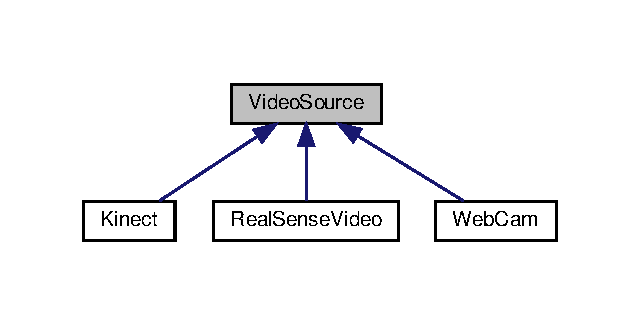
\includegraphics[width=307pt]{class_video_source__inherit__graph}
\end{center}
\end{figure}
\subsection*{Public Member Functions}
\begin{DoxyCompactItemize}
\item 
\mbox{\label{class_video_source_ae18f07760d917884b62d0da6ea2efaee}} 
virtual cv\+::\+Mat {\bfseries get\+Color\+Feed} ()
\item 
\mbox{\label{class_video_source_aba297efc2b09e3534490bf1d02eb84c3}} 
virtual cv\+::\+Mat {\bfseries get\+Depth\+Feed} ()
\item 
\mbox{\label{class_video_source_a9ee8f65394d627443b41f7765f20e20e}} 
virtual cv\+::\+Mat {\bfseries get\+Original\+Depth} ()
\item 
\mbox{\label{class_video_source_a96e2fde5f81c19163831070c34b6d2c8}} 
virtual cv\+::\+Mat {\bfseries get\+Mapped\+Feed} ()
\item 
\mbox{\label{class_video_source_ab5090a635efeb4e8087ba57405f08f32}} 
virtual void {\bfseries update} ()
\item 
\mbox{\label{class_video_source_a6b15d80d574803453f5fec377de02bb4}} 
virtual bool {\bfseries is\+Running} ()
\item 
\mbox{\label{class_video_source_a5adefd9f8be29bb4e0dda8acfd8b7b34}} 
virtual bool {\bfseries has\+Depth\+Source} ()
\item 
\mbox{\label{class_video_source_a4afeab48c5bd2d1d2f07e6a2df0d28f5}} 
virtual std\+::string {\bfseries get\+Time\+Stamp} ()
\item 
\mbox{\label{class_video_source_a99713fa4a77b086b70c5383966288ab9}} 
virtual int {\bfseries get\+Time\+Position} ()
\item 
\mbox{\label{class_video_source_a8f9438a3d5a1599d330bc4bfe1610984}} 
virtual double {\bfseries get\+Exact\+Time\+Position} ()
\item 
\mbox{\label{class_video_source_a47b9dfa3b2719769e514f3360cabb84d}} 
virtual std\+::pair$<$ int, int $>$ {\bfseries get\+Screen\+Size} ()
\end{DoxyCompactItemize}


The documentation for this class was generated from the following file\+:\begin{DoxyCompactItemize}
\item 
controller/sources/Video\+Source.\+h\end{DoxyCompactItemize}

\section{Web\+Cam Class Reference}
\label{class_web_cam}\index{Web\+Cam@{Web\+Cam}}


Inheritance diagram for Web\+Cam\+:
\nopagebreak
\begin{figure}[H]
\begin{center}
\leavevmode
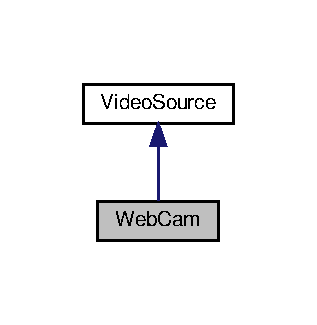
\includegraphics[width=152pt]{class_web_cam__inherit__graph}
\end{center}
\end{figure}


Collaboration diagram for Web\+Cam\+:
\nopagebreak
\begin{figure}[H]
\begin{center}
\leavevmode
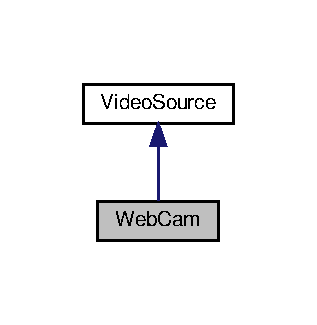
\includegraphics[width=152pt]{class_web_cam__coll__graph}
\end{center}
\end{figure}
\subsection*{Public Member Functions}
\begin{DoxyCompactItemize}
\item 
\mbox{\label{class_web_cam_afe33019aa4a2cbf492c67d70ec95a9be}} 
cv\+::\+Mat {\bfseries get\+Color\+Feed} ()
\item 
\mbox{\label{class_web_cam_a0c177c80bb84d41f2a79240f1e15989b}} 
cv\+::\+Mat {\bfseries get\+Depth\+Feed} ()
\item 
\mbox{\label{class_web_cam_acf080531c8633a52566f09e5c4c33f74}} 
cv\+::\+Mat {\bfseries get\+Original\+Depth} ()
\item 
\mbox{\label{class_web_cam_ab2192287069a02c760b1f097e552ad1f}} 
cv\+::\+Mat {\bfseries get\+Mapped\+Feed} ()
\item 
\mbox{\label{class_web_cam_a2edeaf1bb8cd9f8cb32bd59b79a2d94a}} 
void {\bfseries update} ()
\item 
\mbox{\label{class_web_cam_a369f819e5e6c38b6bb918e5eaefe4913}} 
bool {\bfseries has\+Depth\+Source} ()
\item 
\mbox{\label{class_web_cam_ad34c9510ff27c2bb7c612b1354dcb0a5}} 
std\+::string {\bfseries get\+Time\+Stamp} ()
\item 
\mbox{\label{class_web_cam_a33019db4995dfa30539d8992b0a91a2b}} 
int {\bfseries get\+Time\+Position} ()
\item 
\mbox{\label{class_web_cam_aa2e19da066a26f14dbb4a0533750f691}} 
double {\bfseries get\+Exact\+Time\+Position} ()
\item 
\mbox{\label{class_web_cam_a59eda3f925331c7011830f8da46a45f5}} 
std\+::pair$<$ int, int $>$ {\bfseries get\+Screen\+Size} ()
\end{DoxyCompactItemize}


The documentation for this class was generated from the following files\+:\begin{DoxyCompactItemize}
\item 
controller/sources/Web\+Cam.\+h\item 
controller/sources/Web\+Cam.\+cpp\end{DoxyCompactItemize}

\section{Yolo Class Reference}
\label{class_yolo}\index{Yolo@{Yolo}}


Inheritance diagram for Yolo\+:
\nopagebreak
\begin{figure}[H]
\begin{center}
\leavevmode
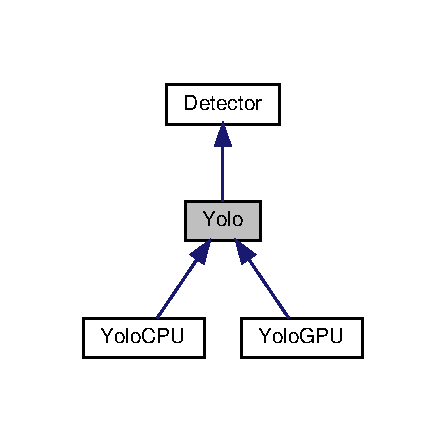
\includegraphics[width=214pt]{class_yolo__inherit__graph}
\end{center}
\end{figure}


Collaboration diagram for Yolo\+:
\nopagebreak
\begin{figure}[H]
\begin{center}
\leavevmode
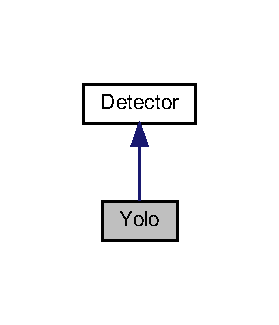
\includegraphics[width=134pt]{class_yolo__coll__graph}
\end{center}
\end{figure}
\subsection*{Additional Inherited Members}


The documentation for this class was generated from the following file\+:\begin{DoxyCompactItemize}
\item 
model/reco\+Activite/reco\+Image/cnn/Yolo.\+h\end{DoxyCompactItemize}

\section{Yolo\+C\+PU Class Reference}
\label{class_yolo_c_p_u}\index{Yolo\+C\+PU@{Yolo\+C\+PU}}


Inheritance diagram for Yolo\+C\+PU\+:
\nopagebreak
\begin{figure}[H]
\begin{center}
\leavevmode
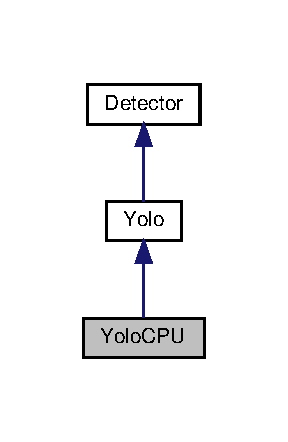
\includegraphics[width=138pt]{class_yolo_c_p_u__inherit__graph}
\end{center}
\end{figure}


Collaboration diagram for Yolo\+C\+PU\+:
\nopagebreak
\begin{figure}[H]
\begin{center}
\leavevmode
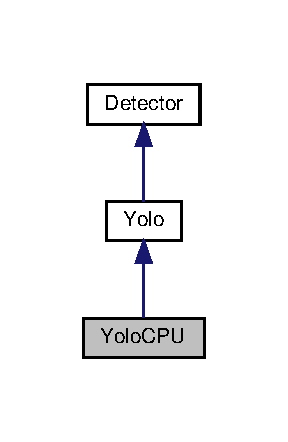
\includegraphics[width=138pt]{class_yolo_c_p_u__coll__graph}
\end{center}
\end{figure}
\subsection*{Public Member Functions}
\begin{DoxyCompactItemize}
\item 
\mbox{\label{class_yolo_c_p_u_af9df13a7e255a3938a75902b690c4135}} 
{\bfseries Yolo\+C\+PU} (float \+\_\+prob, std\+::map$<$ std\+::string, std\+::string $>$ setting)
\item 
\mbox{\label{class_yolo_c_p_u_a79e51bfb44edafc29942c8482d134c27}} 
std\+::vector$<$ \textbf{ Detected\+Object} $>$ {\bfseries find\+Objects} (cv\+::\+Mat color, cv\+::\+Mat depth)
\item 
\mbox{\label{class_yolo_c_p_u_a96e2dd036015132b351e0ce28376e5fe}} 
std\+::string {\bfseries get\+Detector\+Type} ()
\item 
\mbox{\label{class_yolo_c_p_u_ac448b664d5eb80a2efa34536dccec142}} 
void {\bfseries deserialize} (std\+::map$<$ std\+::string, std\+::string $>$ stream)
\end{DoxyCompactItemize}


The documentation for this class was generated from the following files\+:\begin{DoxyCompactItemize}
\item 
model/reco\+Activite/reco\+Image/cnn/Yolo\+C\+P\+U.\+h\item 
model/reco\+Activite/reco\+Image/cnn/Yolo\+C\+P\+U.\+cpp\end{DoxyCompactItemize}

\section{Yolo\+G\+PU Class Reference}
\label{class_yolo_g_p_u}\index{Yolo\+G\+PU@{Yolo\+G\+PU}}


Inheritance diagram for Yolo\+G\+PU\+:
\nopagebreak
\begin{figure}[H]
\begin{center}
\leavevmode
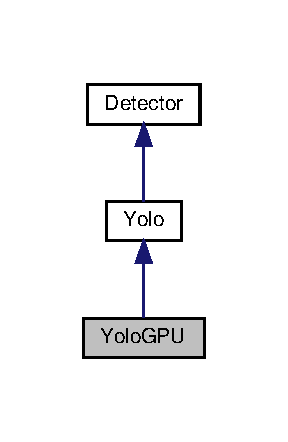
\includegraphics[width=138pt]{class_yolo_g_p_u__inherit__graph}
\end{center}
\end{figure}


Collaboration diagram for Yolo\+G\+PU\+:
\nopagebreak
\begin{figure}[H]
\begin{center}
\leavevmode
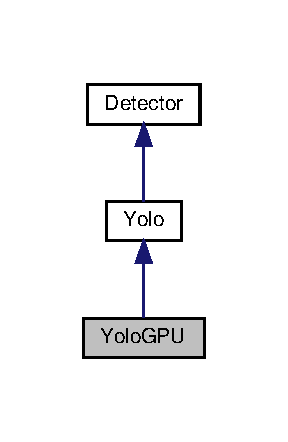
\includegraphics[width=138pt]{class_yolo_g_p_u__coll__graph}
\end{center}
\end{figure}
\subsection*{Public Member Functions}
\begin{DoxyCompactItemize}
\item 
\mbox{\label{class_yolo_g_p_u_a64a5bed90f906a31b6b63eb1efca8024}} 
{\bfseries Yolo\+G\+PU} (float \+\_\+prob, std\+::map$<$ std\+::string, std\+::string $>$ setting)
\item 
\mbox{\label{class_yolo_g_p_u_af6542f94980b65ed5adcfee54256cee9}} 
std\+::vector$<$ \textbf{ Detected\+Object} $>$ {\bfseries find\+Objects} (cv\+::\+Mat color, cv\+::\+Mat depth)
\item 
\mbox{\label{class_yolo_g_p_u_a567132c86a6e9be7e1103cecbceb7915}} 
std\+::string {\bfseries get\+Detector\+Type} ()
\item 
\mbox{\label{class_yolo_g_p_u_adb678816bd5a47b6ad8b2461a358d5fe}} 
void {\bfseries deserialize} (std\+::map$<$ std\+::string, std\+::string $>$ stream)
\end{DoxyCompactItemize}


The documentation for this class was generated from the following files\+:\begin{DoxyCompactItemize}
\item 
model/reco\+Activite/reco\+Image/cnn/Yolo\+G\+P\+U.\+h\item 
model/reco\+Activite/reco\+Image/cnn/Yolo\+G\+P\+U.\+cpp\end{DoxyCompactItemize}

\chapter{File Documentation}
\section{controller/\+Manage\+Source\+Video.h File Reference}
\label{_manage_source_video_8h}\index{controller/\+Manage\+Source\+Video.\+h@{controller/\+Manage\+Source\+Video.\+h}}


Select the good source video including size and handle update.  


{\ttfamily \#include \char`\"{}sources/\+Video\+Source.\+h\char`\"{}}\newline
{\ttfamily \#include \char`\"{}sources/\+Real\+Sense.\+h\char`\"{}}\newline
{\ttfamily \#include \char`\"{}sources/\+Real\+Sense\+Video.\+h\char`\"{}}\newline
{\ttfamily \#include \char`\"{}sources/\+Kinect.\+h\char`\"{}}\newline
{\ttfamily \#include \char`\"{}sources/\+Web\+Cam.\+h\char`\"{}}\newline
{\ttfamily \#include $<$map$>$}\newline
{\ttfamily \#include $<$string$>$}\newline
{\ttfamily \#include $<$opencv2/opencv.\+hpp$>$}\newline
{\ttfamily \#include $<$list$>$}\newline
{\ttfamily \#include $<$cstdlib$>$}\newline
{\ttfamily \#include $<$vector$>$}\newline
{\ttfamily \#include $<$iostream$>$}\newline
{\ttfamily \#include $<$algorithm$>$}\newline
{\ttfamily \#include \char`\"{}Subject.\+h\char`\"{}}\newline
{\ttfamily \#include \char`\"{}../model/\+Observer.\+h\char`\"{}}\newline
Include dependency graph for Manage\+Source\+Video.\+h\+:
\nopagebreak
\begin{figure}[H]
\begin{center}
\leavevmode
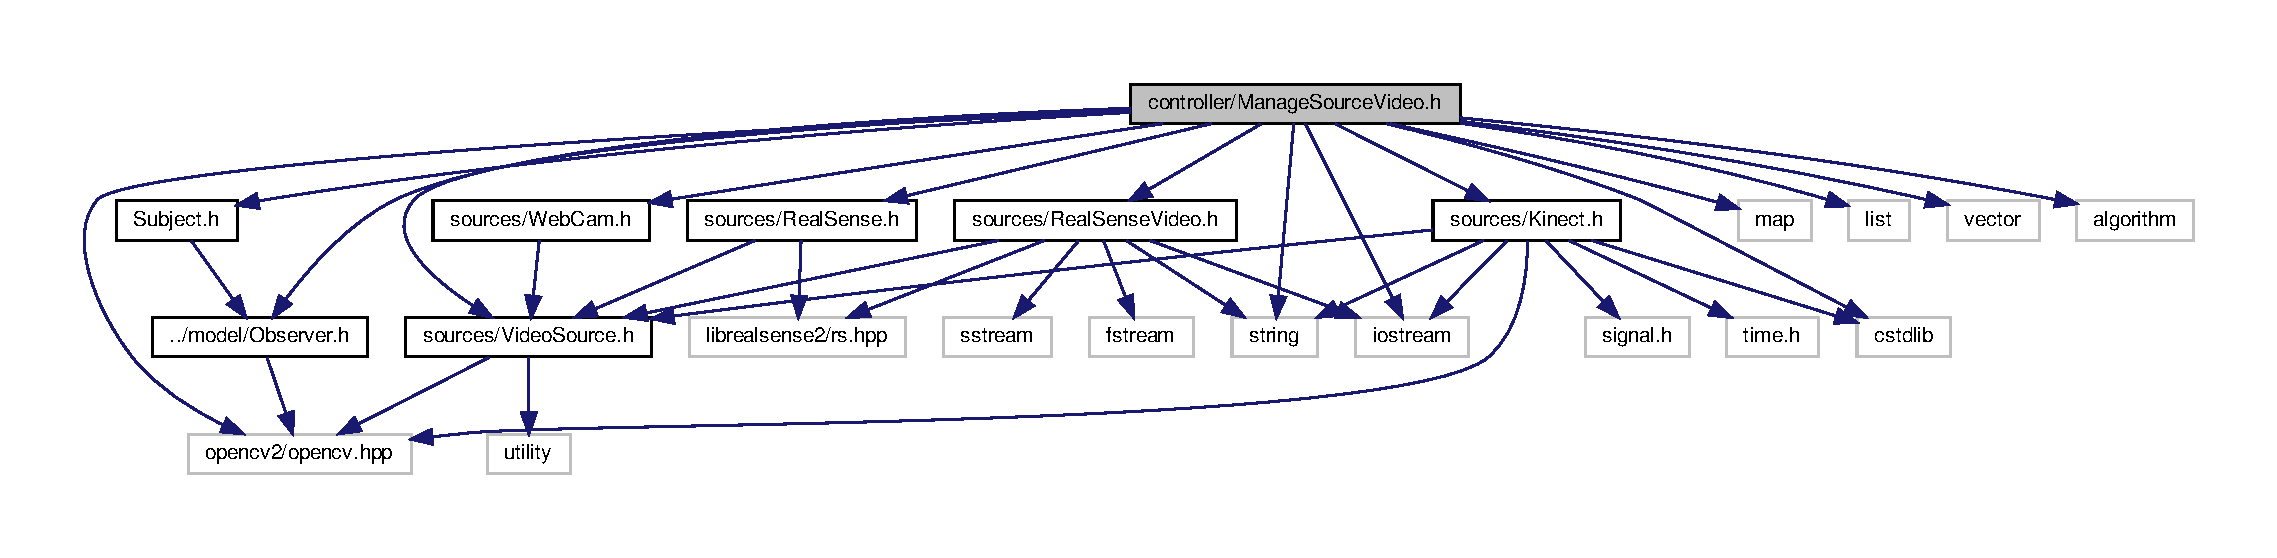
\includegraphics[width=350pt]{_manage_source_video_8h__incl}
\end{center}
\end{figure}
This graph shows which files directly or indirectly include this file\+:
\nopagebreak
\begin{figure}[H]
\begin{center}
\leavevmode
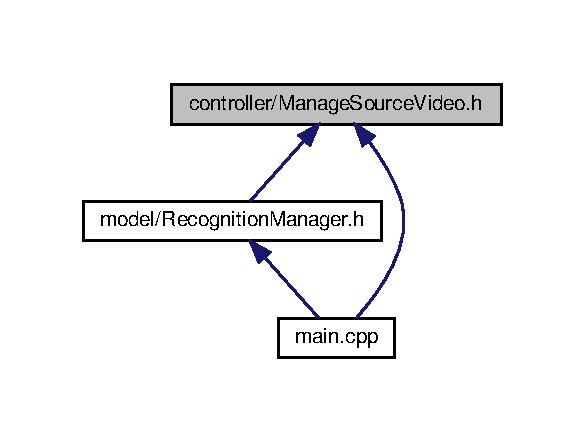
\includegraphics[width=281pt]{_manage_source_video_8h__dep__incl}
\end{center}
\end{figure}
\subsection*{Classes}
\begin{DoxyCompactItemize}
\item 
class \textbf{ Manage\+Source\+Video}
\end{DoxyCompactItemize}


\subsection{Detailed Description}
Select the good source video including size and handle update. 

\begin{DoxyAuthor}{Author}
Mathieu Gravel 
\end{DoxyAuthor}
\begin{DoxyVersion}{Version}
1.\+0 
\end{DoxyVersion}
\begin{DoxyDate}{Date}
13 June 2019 
\end{DoxyDate}

\section{main.\+cpp File Reference}
\label{main_8cpp}\index{main.\+cpp@{main.\+cpp}}


\doxyref{main.\+cpp}{p.}{main_8cpp} \+: Function launching the entire project  


{\ttfamily \#include $<$iostream$>$}\newline
{\ttfamily \#include $<$map$>$}\newline
{\ttfamily \#include \char`\"{}model/\+Recognition\+Manager.\+h\char`\"{}}\newline
{\ttfamily \#include \char`\"{}view/\+Primary\+Window.\+h\char`\"{}}\newline
{\ttfamily \#include \char`\"{}controller/\+Manage\+Source\+Video.\+h\char`\"{}}\newline
Include dependency graph for main.\+cpp\+:
\nopagebreak
\begin{figure}[H]
\begin{center}
\leavevmode
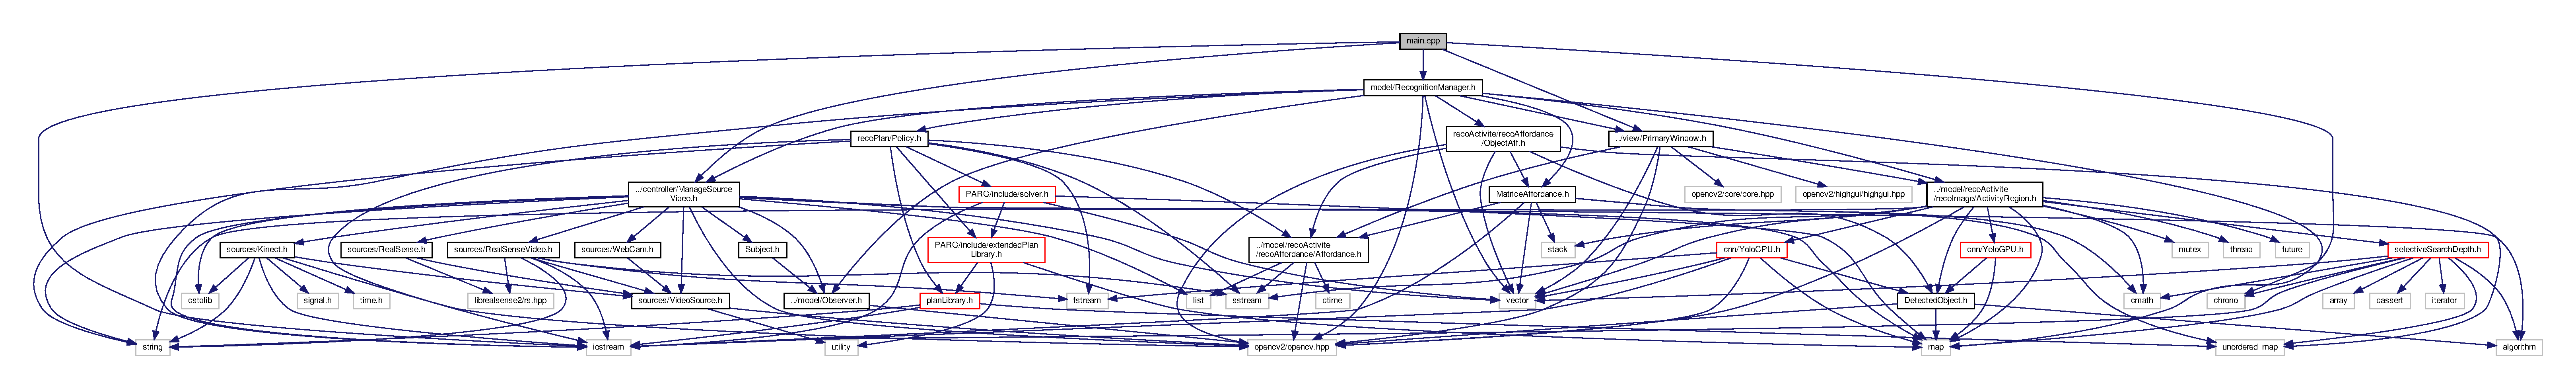
\includegraphics[width=350pt]{main_8cpp__incl}
\end{center}
\end{figure}
\subsection*{Functions}
\begin{DoxyCompactItemize}
\item 
map$<$ string, string $>$ \textbf{ loading\+Setting} (string file\+Setting)
\begin{DoxyCompactList}\small\item\em Model. \end{DoxyCompactList}\item 
int \textbf{ main} (int argc, char $\ast$argv[$\,$])
\end{DoxyCompactItemize}


\subsection{Detailed Description}
\doxyref{main.\+cpp}{p.}{main_8cpp} \+: Function launching the entire project 

\begin{DoxyAuthor}{Author}
Mathieu Gravel -\/ Edited by Alexandre Gonzalvez 
\end{DoxyAuthor}
\begin{DoxyVersion}{Version}
2.\+0 
\end{DoxyVersion}
\begin{DoxyDate}{Date}
25 June 2019
\end{DoxyDate}
Function launching the entire project Create Model, View and Controller Take configuration files in argument 

\subsection{Function Documentation}
\mbox{\label{main_8cpp_ad56b994e44d328f3cd6ae3850d527d74}} 
\index{main.\+cpp@{main.\+cpp}!loading\+Setting@{loading\+Setting}}
\index{loading\+Setting@{loading\+Setting}!main.\+cpp@{main.\+cpp}}
\subsubsection{loading\+Setting()}
{\footnotesize\ttfamily loading\+Setting (\begin{DoxyParamCaption}\item[{string}]{file\+Setting }\end{DoxyParamCaption})}



Model. 

View Controller Function

load setting 
\begin{DoxyParams}{Parameters}
{\em file\+Setting} & \+: name of the file which contains the setting, he as to be in the same folder than the \doxyref{main.\+cpp}{p.}{main_8cpp} \\
\hline
\end{DoxyParams}
\begin{DoxyReturn}{Returns}
setting \+: map$<$string,string$>$ which contain every path and information to use (fisrt String = name\+\_\+of\+\_\+information, second String = information) 
\end{DoxyReturn}
\mbox{\label{main_8cpp_a0ddf1224851353fc92bfbff6f499fa97}} 
\index{main.\+cpp@{main.\+cpp}!main@{main}}
\index{main@{main}!main.\+cpp@{main.\+cpp}}
\subsubsection{main()}
{\footnotesize\ttfamily int main (\begin{DoxyParamCaption}\item[{int}]{argc,  }\item[{char $\ast$}]{argv[$\,$] }\end{DoxyParamCaption})}

Load settings

Display setting in console

Start video acquisition

Create View object (Window if boolean is true) T\+O\+DO\+: Window create \doxyref{Recognition\+Manager}{p.}{class_recognition_manager} when button play is handle (require create a complex window)

Initalize reconnaissance

Start main loop 
\section{model/reco\+Activite/reco\+Affordance/\+Affordance.h File Reference}
\label{_affordance_8h}\index{model/reco\+Activite/reco\+Affordance/\+Affordance.\+h@{model/reco\+Activite/reco\+Affordance/\+Affordance.\+h}}


Evaluates the position between an Object and the Hand.  


{\ttfamily \#include $<$opencv2/opencv.\+hpp$>$}\newline
{\ttfamily \#include $<$ctime$>$}\newline
{\ttfamily \#include $<$sstream$>$}\newline
{\ttfamily \#include $<$list$>$}\newline
Include dependency graph for Affordance.\+h\+:
\nopagebreak
\begin{figure}[H]
\begin{center}
\leavevmode
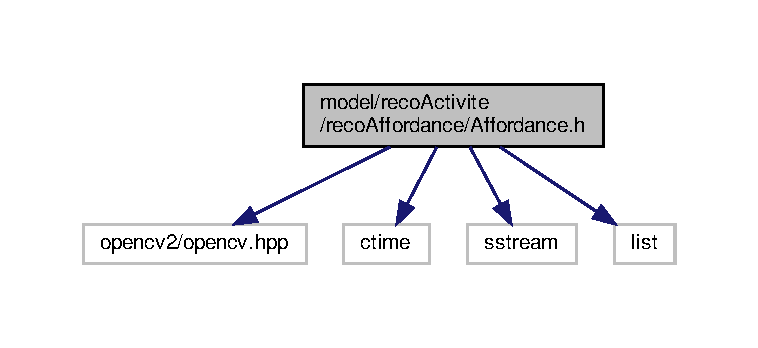
\includegraphics[width=350pt]{_affordance_8h__incl}
\end{center}
\end{figure}
This graph shows which files directly or indirectly include this file\+:
\nopagebreak
\begin{figure}[H]
\begin{center}
\leavevmode
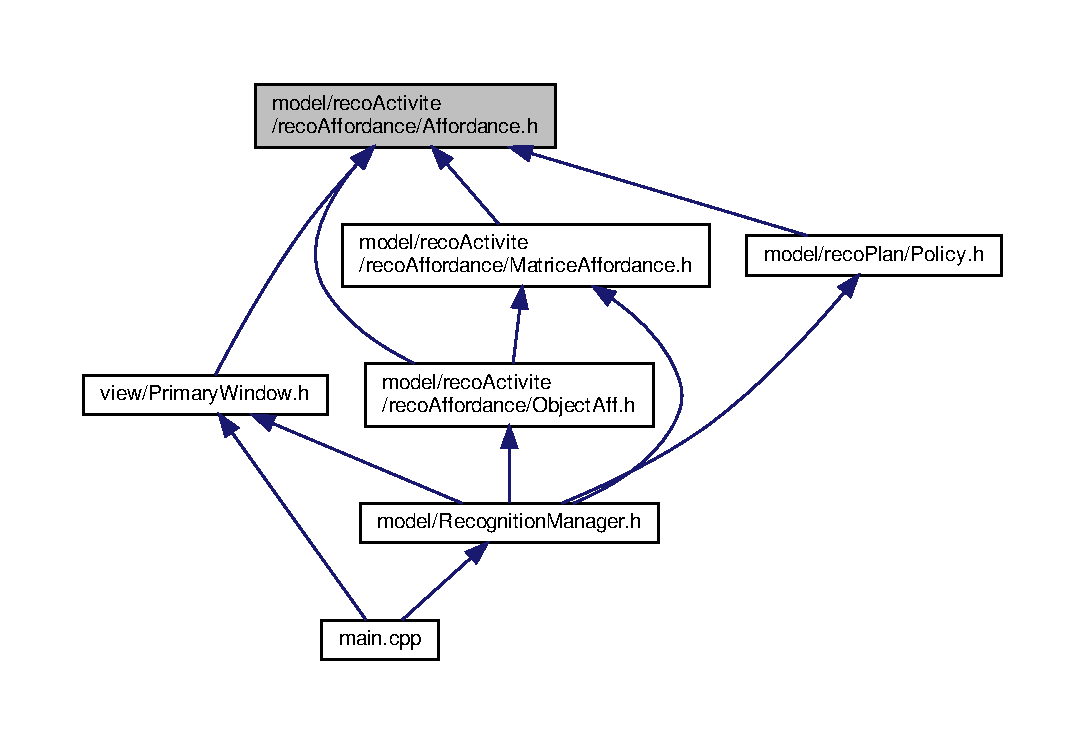
\includegraphics[width=350pt]{_affordance_8h__dep__incl}
\end{center}
\end{figure}
\subsection*{Classes}
\begin{DoxyCompactItemize}
\item 
class \textbf{ Affordance}
\item 
class \textbf{ Affordance\+Time}
\end{DoxyCompactItemize}


\subsection{Detailed Description}
Evaluates the position between an Object and the Hand. 

\begin{DoxyAuthor}{Author}
Mathieu Gravel 
\end{DoxyAuthor}
\begin{DoxyVersion}{Version}

\end{DoxyVersion}
\begin{DoxyDate}{Date}

\end{DoxyDate}
\doxyref{Affordance}{p.}{class_affordance} is used to update regulary the position of the Object during $\ast$ an interaction. It evaluates the distance to the Hand of an Object and is used $\ast$ to add an interaction and its time in the \doxyref{Affordance\+Time}{p.}{class_affordance_time} class. 
\section{model/reco\+Activite/reco\+Affordance/\+Matrice\+Affordance.h File Reference}
\label{_matrice_affordance_8h}\index{model/reco\+Activite/reco\+Affordance/\+Matrice\+Affordance.\+h@{model/reco\+Activite/reco\+Affordance/\+Matrice\+Affordance.\+h}}


keep in memory the last affordances seen (frame in the last 800ms \+: in version 2.\+0) P\+UT in cpp  


{\ttfamily \#include $<$iostream$>$}\newline
{\ttfamily \#include $<$vector$>$}\newline
{\ttfamily \#include $<$unordered\+\_\+map$>$}\newline
{\ttfamily \#include $<$stack$>$}\newline
{\ttfamily \#include $<$cmath$>$}\newline
{\ttfamily \#include \char`\"{}Affordance.\+h\char`\"{}}\newline
Include dependency graph for Matrice\+Affordance.\+h\+:
\nopagebreak
\begin{figure}[H]
\begin{center}
\leavevmode
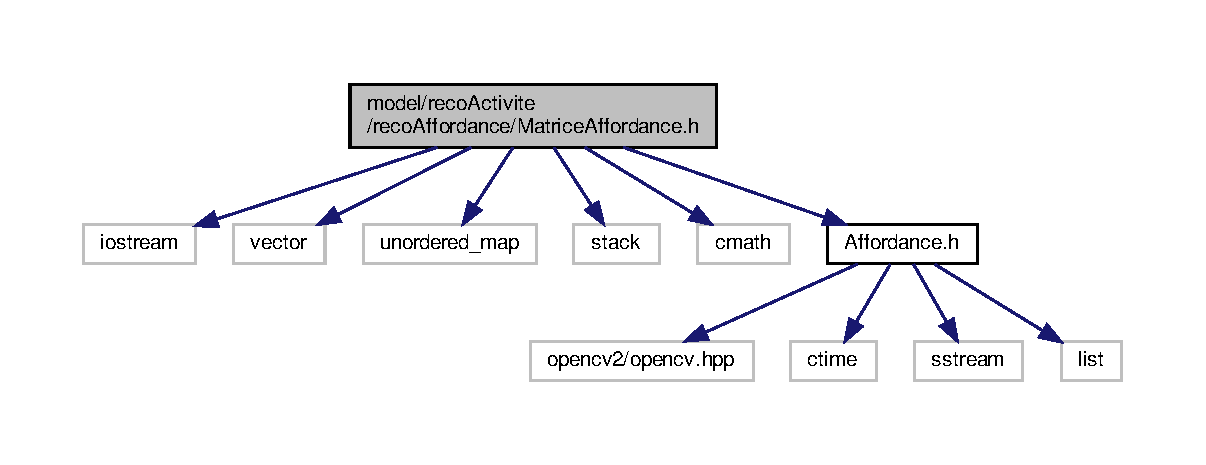
\includegraphics[width=350pt]{_matrice_affordance_8h__incl}
\end{center}
\end{figure}
This graph shows which files directly or indirectly include this file\+:
\nopagebreak
\begin{figure}[H]
\begin{center}
\leavevmode
\includegraphics[width=285pt]{_matrice_affordance_8h__dep__incl}
\end{center}
\end{figure}
\subsection*{Classes}
\begin{DoxyCompactItemize}
\item 
class \textbf{ Matrice\+Affordance}
\end{DoxyCompactItemize}


\subsection{Detailed Description}
keep in memory the last affordances seen (frame in the last 800ms \+: in version 2.\+0) P\+UT in cpp 

\begin{DoxyAuthor}{Author}

\end{DoxyAuthor}
\begin{DoxyVersion}{Version}
2.\+0 
\end{DoxyVersion}
\begin{DoxyDate}{Date}
14/08/2019 
\end{DoxyDate}

\section{model/reco\+Activite/reco\+Affordance/\+Object\+Aff.h File Reference}
\label{_object_aff_8h}\index{model/reco\+Activite/reco\+Affordance/\+Object\+Aff.\+h@{model/reco\+Activite/reco\+Affordance/\+Object\+Aff.\+h}}


select critere to tell if it\textquotesingle{}s could be an affordance  


{\ttfamily \#include $<$opencv2/opencv.\+hpp$>$}\newline
{\ttfamily \#include $<$vector$>$}\newline
{\ttfamily \#include $<$unordered\+\_\+map$>$}\newline
{\ttfamily \#include \char`\"{}Affordance.\+h\char`\"{}}\newline
{\ttfamily \#include \char`\"{}../reco\+Image/\+Detected\+Object.\+h\char`\"{}}\newline
{\ttfamily \#include \char`\"{}Matrice\+Affordance.\+h\char`\"{}}\newline
Include dependency graph for Object\+Aff.\+h\+:
\nopagebreak
\begin{figure}[H]
\begin{center}
\leavevmode
\includegraphics[width=350pt]{_object_aff_8h__incl}
\end{center}
\end{figure}
This graph shows which files directly or indirectly include this file\+:
\nopagebreak
\begin{figure}[H]
\begin{center}
\leavevmode
\includegraphics[width=223pt]{_object_aff_8h__dep__incl}
\end{center}
\end{figure}
\subsection*{Classes}
\begin{DoxyCompactItemize}
\item 
class \textbf{ Object\+Affordances}
\end{DoxyCompactItemize}
\subsection*{Typedefs}
\begin{DoxyCompactItemize}
\item 
\mbox{\label{_object_aff_8h_ab101634c297e47e838e19cd3ee488750}} 
typedef cv\+::\+Rect {\bfseries Region}
\end{DoxyCompactItemize}
\subsection*{Variables}
\begin{DoxyCompactItemize}
\item 
\mbox{\label{_object_aff_8h_ae2924a638c4bc27aa95ed9e715c7dd6f}} 
auto {\bfseries value\+\_\+selector} = [$\,$](auto pair)\{return pair.\+second;\}
\end{DoxyCompactItemize}


\subsection{Detailed Description}
select critere to tell if it\textquotesingle{}s could be an affordance 

\begin{DoxyAuthor}{Author}
Mathieu Gravel 
\end{DoxyAuthor}
\begin{DoxyVersion}{Version}
3.\+0 
\end{DoxyVersion}
\begin{DoxyDate}{Date}

\end{DoxyDate}

\section{model/reco\+Activite/reco\+Image/\+Activity\+Region.h File Reference}
\label{_activity_region_8h}\index{model/reco\+Activite/reco\+Image/\+Activity\+Region.\+h@{model/reco\+Activite/reco\+Image/\+Activity\+Region.\+h}}


interact with Y\+O\+LO which gives detected objects and hands  


{\ttfamily \#include $<$string$>$}\newline
{\ttfamily \#include $<$vector$>$}\newline
{\ttfamily \#include $<$sstream$>$}\newline
{\ttfamily \#include \char`\"{}Detected\+Object.\+h\char`\"{}}\newline
{\ttfamily \#include \char`\"{}selective\+Search\+Depth.\+h\char`\"{}}\newline
{\ttfamily \#include $<$opencv2/opencv.\+hpp$>$}\newline
{\ttfamily \#include $<$mutex$>$}\newline
{\ttfamily \#include $<$thread$>$}\newline
{\ttfamily \#include $<$future$>$}\newline
{\ttfamily \#include \char`\"{}cnn/\+Yolo\+G\+P\+U.\+h\char`\"{}}\newline
{\ttfamily \#include \char`\"{}cnn/\+Yolo\+C\+P\+U.\+h\char`\"{}}\newline
{\ttfamily \#include $<$stack$>$}\newline
{\ttfamily \#include $<$cmath$>$}\newline
{\ttfamily \#include $<$map$>$}\newline
Include dependency graph for Activity\+Region.\+h\+:
\nopagebreak
\begin{figure}[H]
\begin{center}
\leavevmode
\includegraphics[width=350pt]{_activity_region_8h__incl}
\end{center}
\end{figure}
This graph shows which files directly or indirectly include this file\+:
\nopagebreak
\begin{figure}[H]
\begin{center}
\leavevmode
\includegraphics[width=297pt]{_activity_region_8h__dep__incl}
\end{center}
\end{figure}
\subsection*{Classes}
\begin{DoxyCompactItemize}
\item 
class \textbf{ Activity\+Region}
\end{DoxyCompactItemize}


\subsection{Detailed Description}
interact with Y\+O\+LO which gives detected objects and hands 

\begin{DoxyAuthor}{Author}
Mathieu Gravel 
\end{DoxyAuthor}
\begin{DoxyVersion}{Version}
2.\+0 
\end{DoxyVersion}
\begin{DoxyDate}{Date}
8 August 2019 
\end{DoxyDate}

\section{model/reco\+Activite/reco\+Image/\+Detected\+Object.h File Reference}
\label{_detected_object_8h}\index{model/reco\+Activite/reco\+Image/\+Detected\+Object.\+h@{model/reco\+Activite/reco\+Image/\+Detected\+Object.\+h}}


3 class \+: \doxyref{Detected\+Matrice}{p.}{class_detected_matrice}, \doxyref{Detected\+Object}{p.}{class_detected_object}, \doxyref{Detected\+Objects}{p.}{class_detected_objects}  


{\ttfamily \#include $<$opencv2/opencv.\+hpp$>$}\newline
{\ttfamily \#include $<$map$>$}\newline
{\ttfamily \#include $<$algorithm$>$}\newline
Include dependency graph for Detected\+Object.\+h\+:
\nopagebreak
\begin{figure}[H]
\begin{center}
\leavevmode
\includegraphics[width=315pt]{_detected_object_8h__incl}
\end{center}
\end{figure}
This graph shows which files directly or indirectly include this file\+:
\nopagebreak
\begin{figure}[H]
\begin{center}
\leavevmode
\includegraphics[width=350pt]{_detected_object_8h__dep__incl}
\end{center}
\end{figure}
\subsection*{Classes}
\begin{DoxyCompactItemize}
\item 
class \textbf{ Detected\+Matrice}
\item 
class \textbf{ Detected\+Object}
\item 
struct \textbf{ Detected\+Matrices}
\item 
class \textbf{ Detected\+Objects}
\end{DoxyCompactItemize}
\subsection*{Typedefs}
\begin{DoxyCompactItemize}
\item 
\mbox{\label{_detected_object_8h_af71aa18ac8779b4209a86de2e8f226a8}} 
typedef std\+::map$<$ std\+::string, float $>$ {\bfseries Predictions}
\end{DoxyCompactItemize}


\subsection{Detailed Description}
3 class \+: \doxyref{Detected\+Matrice}{p.}{class_detected_matrice}, \doxyref{Detected\+Object}{p.}{class_detected_object}, \doxyref{Detected\+Objects}{p.}{class_detected_objects} 

\begin{DoxyAuthor}{Author}
Mathieu Gravel 
\end{DoxyAuthor}
\begin{DoxyVersion}{Version}
1.\+0 
\end{DoxyVersion}
\begin{DoxyDate}{Date}
13 June 2019
\end{DoxyDate}
\begin{DoxyVerb}DetectedMatrice
    position of an object and prediction

DetectedObject
    position of an object including his color and prediction

DetectedObjects
    vector of detected object\end{DoxyVerb}

\section{model/\+Recognition\+Manager.h File Reference}
\label{_recognition_manager_8h}\index{model/\+Recognition\+Manager.\+h@{model/\+Recognition\+Manager.\+h}}


Manage all project.  


{\ttfamily \#include $<$iostream$>$}\newline
{\ttfamily \#include $<$vector$>$}\newline
{\ttfamily \#include $<$chrono$>$}\newline
{\ttfamily \#include \char`\"{}../controller/\+Manage\+Source\+Video.\+h\char`\"{}}\newline
{\ttfamily \#include \char`\"{}Observer.\+h\char`\"{}}\newline
{\ttfamily \#include $<$opencv2/opencv.\+hpp$>$}\newline
{\ttfamily \#include \char`\"{}../view/\+Primary\+Window.\+h\char`\"{}}\newline
{\ttfamily \#include \char`\"{}reco\+Activite/reco\+Image/\+Activity\+Region.\+h\char`\"{}}\newline
{\ttfamily \#include \char`\"{}reco\+Activite/reco\+Affordance/\+Object\+Aff.\+h\char`\"{}}\newline
{\ttfamily \#include \char`\"{}reco\+Activite/reco\+Affordance/\+Matrice\+Affordance.\+h\char`\"{}}\newline
{\ttfamily \#include \char`\"{}reco\+Plan/\+Policy.\+h\char`\"{}}\newline
Include dependency graph for Recognition\+Manager.\+h\+:
\nopagebreak
\begin{figure}[H]
\begin{center}
\leavevmode
\includegraphics[width=350pt]{_recognition_manager_8h__incl}
\end{center}
\end{figure}
This graph shows which files directly or indirectly include this file\+:
\nopagebreak
\begin{figure}[H]
\begin{center}
\leavevmode
\includegraphics[width=223pt]{_recognition_manager_8h__dep__incl}
\end{center}
\end{figure}
\subsection*{Classes}
\begin{DoxyCompactItemize}
\item 
class \textbf{ Recognition\+Manager}
\end{DoxyCompactItemize}


\subsection{Detailed Description}
Manage all project. 

\begin{DoxyAuthor}{Author}
Alexandre Gonzalvez 
\end{DoxyAuthor}
\begin{DoxyVersion}{Version}
2.\+0 
\end{DoxyVersion}
\begin{DoxyDate}{Date}
8 August 2019
\end{DoxyDate}
Function launching the entire project Define Paramater =$>$ C\+O\+N\+S\+T\+A\+NT (In .cpp) //\+T\+O\+DO \+: put in setting if constant are pertinent Initialize Controller Initialize Activities recognition, Plan recognition Initialize view Start main loop of recognition which update every composant of the program 
\section{model/reco\+Plan/\+P\+A\+R\+C/include/plan\+Library.h File Reference}
\label{plan_library_8h}\index{model/reco\+Plan/\+P\+A\+R\+C/include/plan\+Library.\+h@{model/reco\+Plan/\+P\+A\+R\+C/include/plan\+Library.\+h}}
{\ttfamily \#include $<$iostream$>$}\newline
{\ttfamily \#include $<$unordered\+\_\+set$>$}\newline
{\ttfamily \#include $<$unordered\+\_\+map$>$}\newline
{\ttfamily \#include $<$string$>$}\newline
{\ttfamily \#include \char`\"{}rule.\+h\char`\"{}}\newline
Include dependency graph for plan\+Library.\+h\+:
\nopagebreak
\begin{figure}[H]
\begin{center}
\leavevmode
\includegraphics[width=350pt]{plan_library_8h__incl}
\end{center}
\end{figure}
This graph shows which files directly or indirectly include this file\+:
\nopagebreak
\begin{figure}[H]
\begin{center}
\leavevmode
\includegraphics[width=350pt]{plan_library_8h__dep__incl}
\end{center}
\end{figure}
\subsection*{Classes}
\begin{DoxyCompactItemize}
\item 
class \textbf{ plan\+Library}
\end{DoxyCompactItemize}


\subsection{Detailed Description}
\begin{DoxyAuthor}{Author}
Jean Massardi 
\end{DoxyAuthor}
\begin{DoxyVersion}{Version}
2.\+0 
\end{DoxyVersion}
\begin{DoxyDate}{Date}
8 August 2019 
\end{DoxyDate}

\section{model/reco\+Plan/\+Policy.h File Reference}
\label{_policy_8h}\index{model/reco\+Plan/\+Policy.\+h@{model/reco\+Plan/\+Policy.\+h}}
{\ttfamily \#include $<$string$>$}\newline
{\ttfamily \#include \char`\"{}../reco\+Activite/reco\+Affordance/\+Affordance.\+h\char`\"{}}\newline
{\ttfamily \#include $<$sstream$>$}\newline
{\ttfamily \#include $<$iostream$>$}\newline
{\ttfamily \#include $<$fstream$>$}\newline
{\ttfamily \#include \char`\"{}P\+A\+R\+C/include/extended\+Plan\+Library.\+h\char`\"{}}\newline
{\ttfamily \#include \char`\"{}P\+A\+R\+C/include/plan\+Library.\+h\char`\"{}}\newline
{\ttfamily \#include \char`\"{}P\+A\+R\+C/include/solver.\+h\char`\"{}}\newline
Include dependency graph for Policy.\+h\+:
\nopagebreak
\begin{figure}[H]
\begin{center}
\leavevmode
\includegraphics[width=350pt]{_policy_8h__incl}
\end{center}
\end{figure}
This graph shows which files directly or indirectly include this file\+:
\nopagebreak
\begin{figure}[H]
\begin{center}
\leavevmode
\includegraphics[width=223pt]{_policy_8h__dep__incl}
\end{center}
\end{figure}
\subsection*{Classes}
\begin{DoxyCompactItemize}
\item 
class \textbf{ Policy}
\end{DoxyCompactItemize}


\subsection{Detailed Description}
\begin{DoxyAuthor}{Author}
Mathieu Gravel 
\end{DoxyAuthor}
\begin{DoxyVersion}{Version}

\end{DoxyVersion}
\begin{DoxyDate}{Date}

\end{DoxyDate}

\section{view/\+Primary\+Window.h File Reference}
\label{_primary_window_8h}\index{view/\+Primary\+Window.\+h@{view/\+Primary\+Window.\+h}}


interface of the program  


{\ttfamily \#include $<$vector$>$}\newline
{\ttfamily \#include $<$opencv2/opencv.\+hpp$>$}\newline
{\ttfamily \#include $<$opencv2/core/core.\+hpp$>$}\newline
{\ttfamily \#include $<$opencv2/highgui/highgui.\+hpp$>$}\newline
{\ttfamily \#include \char`\"{}../model/reco\+Activite/reco\+Image/\+Activity\+Region.\+h\char`\"{}}\newline
{\ttfamily \#include \char`\"{}../model/reco\+Activite/reco\+Affordance/\+Affordance.\+h\char`\"{}}\newline
Include dependency graph for Primary\+Window.\+h\+:
\nopagebreak
\begin{figure}[H]
\begin{center}
\leavevmode
\includegraphics[width=350pt]{_primary_window_8h__incl}
\end{center}
\end{figure}
This graph shows which files directly or indirectly include this file\+:
\nopagebreak
\begin{figure}[H]
\begin{center}
\leavevmode
\includegraphics[width=260pt]{_primary_window_8h__dep__incl}
\end{center}
\end{figure}
\subsection*{Classes}
\begin{DoxyCompactItemize}
\item 
class \textbf{ Primary\+Window}
\end{DoxyCompactItemize}


\subsection{Detailed Description}
interface of the program 

\begin{DoxyAuthor}{Author}
Mathieu Gravel Edited by Alexandre Gonzalvez 
\end{DoxyAuthor}
\begin{DoxyVersion}{Version}
2.\+0 
\end{DoxyVersion}
\begin{DoxyDate}{Date}
8 August 2019
\end{DoxyDate}
If boolean = True take a the matrix of color, position of hands and objects in input draw rectangle over it int the matrix and display it Else do nothing TO A\+DD \+: D\+I\+S\+P\+L\+AY display current action and 2 previous or more display next action (most likely) (like 3) display current plan (most likely) (like 3) Alert when the user do an action which is unlikely B\+U\+T\+T\+ON To start the program To choose option (controller(real\+Sense/webcam/video/kinect), ect ... (maybe F\+PS, G\+P\+U/\+C\+PU, langage)) A\+G\+E\+W\+E\+LL \& G\+D\+A\+C/\+U\+Q\+AM \& author (J.\+Massardi/M.Gravel/\+E.\+Beaudry) 
%--- End generated contents ---

% Index
\backmatter
\newpage
\phantomsection
\clearemptydoublepage
\addcontentsline{toc}{chapter}{Index}
\printindex

\end{document}
